%% Use the standard UP-methodology class
%% with French language.
%%
%% You may specify the option 'twoside' or 'oneside' for
%% the document.
%%
%% See the documentation tex-upmethodology on
%% http://www.arakhne.org/tex-upmethodology/
%% for details about the macros that are provided by the class and
%% to obtain the list of the packages that are already included.
\pdfobjcompresslevel 0
\documentclass[english,standardlists]{spimubphdthesis}

% To prevent warning on todo package
\setlength{\marginparwidth}{2cm}

%% Custom commands and packages configuration
%% ------------------
%% Helpers when writing (display the TODO notes and TODO list)
%% ------------------

\usepackage{todonotes}[french]
\usepackage{etoolbox}

\newtoggle{todolist}
\togglefalse{todolist}

\newcommand{\phdseetodo}{\toggletrue{todolist}}
\newcommand{\phdhidetodo}{\togglefalse{todolist}}
\newcommand{\phdtodotoc}{\iftoggle{todolist}{\clearpage\listoftodos}{}}
\newcommand{\phdtodomargin}[2][green]{\iftoggle{todolist}{\todo[color=#1!40]{#2}}{}}
\newcommand{\phdtodo}[2][green]{\iftoggle{todolist}{\todo[inline, color=#1!40]{#2}}{}}
\newcommand{\phdmissingfig}[2]{\missingfigure{#1}}


\usepackage{subcaption}
\usepackage{wrapfig}
\usepackage{pdflscape}
\usepackage{multirow, makecell}
\usepackage{array,booktabs}

%% ----------------------------------------------------------------
\usepackage[xindy,acronym,toc,shortcuts]{glossaries}
\usepackage[xindy]{imakeidx}

%% ----------------------------------------------------------------
%% --- Configure hyperlinks, minitoc, epigraph
%% ----------------------------------------------------------------
\usepackage{xcolor}

\usepackage{minitoc}
\usepackage{epigraph}

% Include the listings-package for code listings
\usepackage{algpseudocode}
\usepackage{algorithm}

\usepackage[T1]{fontenc}
\usepackage[utf8]{inputenc}
\usepackage{csquotes}

\usepackage{amsmath}
\usepackage{bibentry}
\usepackage{cleveref}
\usepackage[inline]{enumitem}
\usepackage{siunitx}
\usepackage{subcaption}
% \usepackage{fancyhdr}
% \pagestyle{fancy}

% \renewcommand{\headrulewidth}{0pt} 
% \fancyhead[LE, LO] {Page \thepage}
% \fancyhead[RE, RO] {Question \the\QuestionNumber}

%%%%%%%%%%%%%%% Parameters
% Custom hyperlinks
\hypersetup{
  colorlinks,
  linkcolor={red!80!black},
  citecolor={blue!70!black},
  urlcolor={blue!50!black},
}

% Length of epigraph
\setlength{\epigraphwidth}{0.7\textwidth}

% Depth of minitoc of 2
\setcounter{minitocdepth}{2}

% Custom list
\newlist{inlinerate}{enumerate*}{1}
\setlist[inlinerate]{label=(\roman*)}

% Custom unit and range
\sisetup{range-phrase=--}
\DeclareSIUnit\px{px}

\nobibliography*

% Custom chapter
\newcommand\unchapter[1]{%
  \chapter*{#1}%
  \chaptermark{#1} 
  \addcontentsline{toc}{chapter}{#1}
  \mtcaddchapter}
  
% Custom title for mini toc contents
\renewcommand{\mtctitle}{Sommaire}

% Custom caption
\DeclareCaptionLabelSeparator{colon}{ : }

% - Use column specifier R/C/L{size} when declaring array to fix column size
\newcolumntype{R}[1]{>{\raggedleft\let\newline\\\arraybackslash\hspace{0pt}}m{#1}}
\newcolumntype{C}[1]{>{\centering\let\newline\\\arraybackslash\hspace{0pt}}m{#1}}
\newcolumntype{L}[1]{>{\raggedright\let\newline\\\arraybackslash\hspace{0pt}}m{#1}}
  
%%%%%%%%%%%%%%% Special macros
\makeglossaries
\makeindex

\makeatletter
\newcommand*{\glsplainhyperlink}[2]{%
  \colorlet{currenttext}{.}% store current text color
  \colorlet{currentlink}{\@linkcolor}% store current link color
  \hypersetup{linkcolor={red!40!black}}% set link color to text color
  \hyperlink{#1}{#2}% create link
  \hypersetup{linkcolor=currentlink}% reset link color to original
}
\let\@glslink\glsplainhyperlink
\makeatother

% -- adding keys for multilingual acronyms
% -- french name and french acronym
\glsaddkey{frshort}
{}% default value
{\glsentryfrshort}
{\Glsentryfrshort}
{\acrfrshort}
{\Acrfrshort}
{\ACRfrshort}

\glsaddkey{frlong}
{}
{\glsentryfrlong}
{\Glsentryfrlong}
{\acrfrlong}
{\Acrfrlong}
{\ACRfrlong}

% -- test if new keys are present in entry
\newcommand*{\glsifhasfrshort}[3]{%
  \ifcsempty{glo@#1@frshort}{#3}{#2}%
}

\newcommand*{\glsifhasfrlong}[3]{%
  \ifcsempty{glo@#1@frlong}{#3}{#2}%
}

\newcommand*{\glsifhasfr}[3]{%
  \glsifhasfrshort{#1}{#2}{\glsifhasfrlong{#1}{#2}{#3}}
}

\newcommand*{\acrshortfr}[1]{%
  \glsifhasfrshort{#1}{\acrfrshort{#1}}{\acrshort{#1}}%
}

\newcommand*{\acrlongfr}[1]{%
  \glsifhasfrlong{#1}{\acrfrlong{#1}}{\acrlong{#1}}%
}

% -- define new acronym style
\newacronymstyle{fracr}
{%
  \GlsUseAcrEntryDispStyle{long-short}%
}%
{% base definition on 'long-short'
  % make some modifications for first use display
  % Singular, no case change:
  \GlsUseAcrStyleDefs{long-short}%
  \renewcommand*{\genacrfullformat}[2]{%
    \glsifhasfr{##1}%
    {%
      \glsentrylong{##1}##2,%
      \space\firstacronymfont{\glsentryshort{##1}}\space%
      (\textit{fr : \glsifhasfrlong{##1}%
        {\glsentryfrlong{##1}##2\glsifhasfrshort{##1}{, \space}{}}{}%
        \glsifhasfrshort{##1}{\glsentryfrshort{##1}}{}})%
    }%
    {%
      \glsentrylong{##1}##2,
      \space(\firstacronymfont{\glsentryshort{##1}})%
    }%
  }%
  % Singular, first letter upper case
  \renewcommand*{\Genacrfullformat}[2]{%
    \glsifhasfr{##1}%
    {%
      \Glsentrylong{##1}##2,
      \space\firstacronymfont{\glsentryshort{##1}}\space
      (\textit{fr : \glsifhasfrlong{##1}%
        {\glsentryfrlong{##1}##2\glsifhasfrshort{##1}{, \space}{}}{}%
        \glsifhasfrshort{##1}{\glsentryfrshort{##1}}{}})%
    }%
    {%
      \Glsentrylong{##1}##2,
      \space(\firstacronymfont{\glsentryshort{##1}})%
    }%
  }%
  % Plural, no case change:
  \renewcommand*{\genplacrfullformat}[2]{%
    \glsifhasfr{##1}%
    {%
      \glsentrylongpl{##1}##2,
      \space\firstacronymfont{\glsentryshortpl{##1}}\space,
      (\textit{fr : \glsifhasfrlong{##1}%
        {\glsentryfrlong{##1}##2\glsifhasfrshort{##1}{, \space}{}}{}%
        \glsifhasfrshort{##1}{\glsentryfrshort{##1}}{}})%
    }%
    {%
      \glsentrylongpl{##1}##2,
      \space(\firstacronymfont{\glsentryshortpl{##1}})%
    }%
  }%
  % Plural, first letter upper case:
  \renewcommand*{\Genplacrfullformat}[2]{%
    \glsifhasfr{##1}%
    {%
      \Glsentrylongpl{##1}##2,
      \space\firstacronymfont{\glsentryshortpl{##1}}\space,
      (\textit{fr : \glsifhasfrlong{##1}%
        {\glsentryfrlong{##1}##2\glsifhasfrshort{##1}{, \space}{}}{}%
        \glsifhasfrshort{##1}{\glsentryfrshort{##1}}{}})%
    }%
    {%
      \Glsentrylongpl{##1}##2,
      \space(\firstacronymfont{\glsentryshortpl{##1}})%
    }%
  }%
}

\setacronymstyle{fracr}

\newglossarystyle{listfracr}{%
  \setglossarystyle{list}%
  \renewcommand*{\glossentry}[2]{%
  \item[\glsentryitem{##1}%
    \glstarget{##1}{\glossentryname{##1}}]
    \glossentrydesc{##1}%
    \glsifhasfrlong{##1}%
      {\space(\textit{fr : \glsentryfrlong{##1}}\glsifhasfrshort{##1}{,\space}{)}}%
      {\glsifhasfrshort{##1}{\space(\textit{fr : }}{}}%
    \glsifhasfrshort{##1}{\textit{\glsentryfrshort{##1}})}{}%
    \glspostdescription\space ##2}%
}

% -- define fancy quotes
\definecolor{quotemark}{gray}{0.7}
\makeatletter
\def\fquote{%
    \@ifnextchar[{\fquote@i}{\fquote@i[]}%]
           }%
\def\fquote@i[#1]{%
    \def\tempa{#1}%
    \@ifnextchar[{\fquote@ii}{\fquote@ii[]}%]
                 }%
\def\fquote@ii[#1]{%
    \def\tempb{#1}%
    \@ifnextchar[{\fquote@iii}{\fquote@iii[]}%]
                      }%
\def\fquote@iii[#1]{%
    \def\tempc{#1}%
    \vspace{1em}%
    \noindent%
    \begin{list}{}{%
         \setlength{\leftmargin}{0.55\textwidth}%
         \setlength{\rightmargin}{0.01\textwidth}%
                  }%
         \item[]%
         \begin{picture}(0,0)%
         \put(-15,-5){\makebox(0,0){\scalebox{3}{\textcolor{quotemark}{``}}}}%
         \end{picture}%
         \begingroup\itshape}%
 %%%%********************************************************************
 \def\endfquote{%
 \endgroup\par%
 \makebox[0pt][l]{%
 \hspace{0.4\textwidth}%
 \begin{picture}(0,0)(0,0)% 
	 \put(15,15){\makebox(0,0){%
	 \scalebox{3}{\color{quotemark}''}}}%
 \end{picture}}%
 \ifx\tempa\empty%
 \else%
    \ifx\tempc\empty%  
       \hfill\rule{100pt}{0.5pt}\\\mbox{}\hfill\tempa,\ \emph{\tempb}%
   \else%		
       \hfill\rule{100pt}{0.5pt}\\\mbox{}\hfill\tempa,\ \emph{\tempb},\ \tempc%
   \fi\fi\par%
   \vspace{0.5em}%
 \end{list}%
 }%
\makeatother

%% ----------------------------------------------------------------
%% --- change font
%%
%% --- float with adjusting left / right margins using
%% \begin{figure}[t]
%%  \centering
%%  \addtolength{\leftskip}{-3cm}
%%  \addtolength{\rightskip}{-3cm}
%%  % figure content
%% \end{figure}
%%
%% --- custom ("pro") arrays with \toprule, \midrule, \cmidrule and \bottomrule
%% ----------------------------------------------------------------
\renewcommand{\familydefault}{\rmdefault}
\makeatletter
\newcommand*{\centerfloat}{%
  \parindent \z@
  \leftskip \z@ \@plus 1fil \@minus \textwidth
  \rightskip\leftskip
  \parfillskip \z@skip}
\makeatother



%\loadglsentries[main]{glossaire}
\loadglsentries[\glsronymtype]{resources/acronyms}

%%--------------------
%% Set the title, subtitle, defense date, and
%% the registration number of the PhD thesis.
%% The optional parameter is the subtitle of the PhD thesis.
%% The first mandatory parameter is the title of the PhD thesis.
%% The second mandatory parameter is the date of the PhD defense.
%% The third mandatory parameter is the location/city of the PhD defense.
%% The forth mandatory parameter is the reference number given by
%% the University Library after the PhD defense.
\declarethesis[]{Titre de la thèse}{Date de soutenance}{Dijon}{XXX}

%%--------------------
%% Set the author of the PhD thesis
\addauthor[romain.cendre@gmail.com]{Romain}{CENDRE}

%%--------------------
%% Add a member of the jury
%%
%% CAUTION 1: If a Jury member is not present during the defense,
%%            she/he must be in the list of the Jury members.
%%            Only the reviewers and the members who are present during the defense must
%%            appear in the Jyry member list.
%% CAUTION 2: After your defense, you must assign the role "Pr\'esident" to
%%            the Jury member who have been the President of the Jury.
%% CAUTION 3: The recommended order for the Jury members is:
%%            President, Reviewer(s), Examiner(s), Director(s),
%%            Other supervisor(s), Invited person(s).
%% \addjury{Firstname}{Lastname}{Role in the jury}{Position}
\addjury{Prenom}{Nom}{Rapporteur}{Professeur, Université XXX}
\addjury{Prenom}{Nom}{Rapporteur}{Professeur, Université XXX}
\addjury{Franck}{MARZANI}{Directeur de thèse}{Professeur des Universités, Université de Bourgogne}
\addjury{Alamin}{MANSOURI}{Co-encadrant}{Professeur des Universités, Université Bourgogne}

%%--------------------
%% Change style of the table of the jury
%% \Set{jurystyle}{put macros for the style}
%\Set{jurystyle}{\small}

%%--------------------
%% Set the English abstract
\thesisabstract[english]{
English resume
}

%%--------------------
%% Set the English keywords. They only appear if
%% there is an English abstract
\thesiskeywords[english]{Dermatology, Lentigo, Machine Learning, Deep Learning, Image processing, Image classification, Multimodality, Data fusion, Reflectance Confocal Microscopy}

%%--------------------
%% Set the French abstract
\thesisabstract[french]{
Résumé français
}

%%--------------------
%% Set the French keywords. They only appear if
%% there is an French abstract
\thesiskeywords[french]{Dermatologie, Lentigo, Apprentissage automatique, Apprentissage profond, Traitement d'image, Classification d'images, Multimodalité, Fusion de données, Microscopie confocale par réflectance}

%%--------------------
%% Change the layout and the style of the text of the "primary" abstract.
%% If your document is written in French, the primary abstract is in French,
%% otherwise it is in English.
%\Set{primaryabstractstyle}{\tiny}

%%--------------------
%% Change the layout and the style of the text of the "secondary" abstract.
%% If your document is written in French, the secondary abstract is in English,
%% otherwise it is in French.
%\Set{secondaryabstractstyle}{\tiny}

%%--------------------
%% Change the layout and the style of the text of the "primary" keywords.
%% If your document is written in French, the primary keywords are in French,
%% otherwise they are in English.
%\Set{primarykeywordstyle}{\tiny}

%%--------------------
%% Change the layout and the style of the text of the "secondary" keywords.
%% If your document is written in French, the secondary keywords are in English,
%% otherwise they are in French.
%\Set{secondarykeywordstyle}{\tiny}

%%--------------------
%% Change the speciality of the PhD thesis
\Set{speciality}{Informatique}

%%--------------------
%% Change the institution
\Set{universityname}{Université de Bourgogne}

%%--------------------
%% Clear the list of the laboratories
\resetlaboratories

%%--------------------
%% Add the laboratory where the thesis was made
\addlaboratory{ImVia}

%%--------------------
%% Clear the list of the partner/sponsor logos
\resetpartners

%%--------------------
%% Add the logos of the partners or the sponsors on the front page
%%
%% CAUTION 1: At least, the logo of the University should appear (UB)
%%
\addpartner{resources/logos/ub}

%%--------------------
%% Change the message on the backcover.
\Set{backcovermessage}{
  % Ajouter logos partenaires de la thèse
}

\begin{document}
\dominitoc

%%--------------------
%% The following line does nothing until
%% the class option 'nofrontmatter' is given.
%\frontmatter

%%--------------------
%% The following line permits to add a chapter for "acknowledgements"
%% at the beginning of the document. This chapter has not a chapter
%% number (using the "star-ed" version of \chapter) to prevent it to
%% be in the table of contents

\parbox[t]{\textwidth}
{
    \vspace{1.5cm}
	\begin{fquote}[Bernard de Chartres][\textit{Gloses sur Priscien}]
		Des nains sur des épaules de géants.
	\end{fquote}	
}
	
\chapter*{Remerciements}
Comme l'usage le permet, je profite de ces quelques paragraphes pour exprimer, par ces éléments subjectifs mais pourtant cruciaux à l'élaboration d'une thèse, ma gratitude envers celles et ceux qui m'ont soutenu durant l'élaboration de ce projet.\par

Ainsi, ces travaux ont été rendus possibles grâce au Conseil Régional de Bourgogne Franche Comté et le \gls{feder} dans le cadre de l'initiative des \gls{jce}. Je tiens naturellement à leur exprimer mes plus sincères remerciements, sans quoi toute cette aventure n'aurait pas pu voir le jour. En effet, ces trois années auront été l'occasion d'une expérience scientifique, mais également de formations intenses à l'administration des entreprises auprès de l'IAE de Dijon et de la Business School of Burgundy.\par

Il est important de débuter ces remerciements envers ceux qui ont initié ce travail, Messieurs Franck Marzani et Alamin Mansouri, et qui ont soutenu ma candidature à ce financement et à ce projet commun. Par ailleurs, je les remercie également pour leur précieux soutien moral et pour leur oreille attentive malgré les nombreuses responsabilités qui leur incombent. Par cette même occasion, je dédie mes remerciements à deux médecins, Jean-Luc Perrot et Elisa Cinotti, dont la participation, le temps consacré, ainsi que la bonne humeur auront été essentiel à la réussite de ce projet.\par

Également, un grand merci aux membres du jury... mais également à mes rapporteurs qui ont eu à la tâche\par

Ainsi, je remercie tout naturellement ma structure d'accueil, le laboratoire \gls{imvia}, et l'ensemble de ses membres qui m'auront permis de travailler dans un cadre des plus favorables durant ces trois années. Ainsi pour toutes les démarches administratives, je citerai Fabienne Blaise, Anne Fournier, et Khadija Jourani qui m'ont épaulé pour la plupart d'entre elles et aurons été d'une réactivité à toute épreuve. Notre quotidien serait fortement impacté sans une équipe soudée, ainsi je remercie Cyrille Migniot, Fan Yang, Barthelemy Heyrman, et Julien Dubois qui ont beaucoup contribué à ce dernier. J'exprime également une pensée envers Dominique Ginhac et Barthelemy Heyrman qui ont gracieusement mis à ma disposition des ressources informatiques sans lesquelles ce travail aurait été difficile à réaliser.\par

J'ai une pensée toute particulière pour l'ensemble de mes collègues de laboratoire et de Master, qui par leur présence m'ont rendu ces trois années plus conviviales. C'est avec nostalgie que je repense à d'anciennes discussions en compagnie de Abdelali Douiyek et Mustapha Bouderbane, mes anciens compagnons "d'îlot", remplacé par une nouvelle équipe tout aussi sympathique avec Abir Zendagui, Marvin Nurit et Yuly Castro. Également, je citerai Margarita Khokhlova, Pierre Bonazza, Alpha Liu et Antoine Léger pour nos discussions passionné et constructifs autour de l'apprentissage automatique et profond; Dans ce registre de discussions passionnées, un merci à Alpha Liu et David Lewis pour nos échanges sur des thèmes très variés en anglais, ce qui me permet d'entretenir cette langue; enfin je termine des collègues dont le passage m'aura marqué, c'est notamment le cas pour Axel Moinet, Serge Bobbia, Yoan Marin et Duncan Luguern.\par

Que serait une thèse sans quelques soupapes pour évacuer le stress accumulé. Je profite de ce paragraphe pour dresser quelques attentions à deux membres : Fan Yang et Yannick Benezeth, qui n'ont jamais hésité à me remonter le moral dans les moments les plus durs. J'ai évoqué des soupapes, la course à pied est l'une d'entre elles, et c'est donc une attention toute particulière que je porte à notre noyau de course soudé composé de Fan Yang, Yannick Benezeth, Cédric Démonceaux, Alexandre Krebs, Abir Zendagui et Rita Meziati. Enfin, c'est grâce à une personne de passage au laboratoire \gls{imvia} et passionné de cross-country, que j'ai pu découvrir les paysages de Bourgogne, je te remercie pour cela Olivier Roblin.\par

Mes propos sont évasifs à ce sujet, et pourtant le Master aura été contrainte et évasion, et m'aura permis des rencontres impossibles dans d'autres circonstance. Ainsi, je vous remercie Antoine Greisner, Jérémie Vion et Augustin Cognacq d'avoir été de fidèles collègues de travail et amis. Dans une catégorie similaire, mais pourtant lié à ces enseignements de Master, je souhaiterais citer mes collègues de \gls{jce} dont Alicia Froidurot, Garance Dejouy et Anne Berrou font partie. Je les considère avant tout comme des compagnons de galère car nous avons partagé de nombreuses périodes délicates, tiraillé entre nos responsabilités au laboratoire et envers ces cours.\par
 
Bien évidemment, je ne peux finir ces remerciements sans oublier mes proches qui ont été constamment présent à mes côtés, tant durant les moments joyeux que les plus difficiles et ont eus des paroles réconfortantes. Tout d'abord, mes amis avec qui il n'a pas été facile de garder contact malgré la distance et pour lesquels j'ai pu assister aux diverses étapes de leur vies, et ce jusqu'à devenir une famille. Enfin, je terminerais par mon cercle le plus proche, incluant mes parents qui m'ont porté durant toutes ces années et encouragé à aller de l'avant. Je me sens bien souvent ingrat de ne pas leur témoigner la même attention qu'il me porte. Et je ne peux oublier ma compagne, Claire, qui m'épaule dans l'ombre depuis maintenant 5 années et qui me suis au quotidien, et dont la présence me permet de surmonter maintes périodes difficiles. C'est avec joie que je te porte un grand merci.\par
		
%%--------------------
%% Include a general table of contents
\tableofcontents

%%--------------------
%% The content of the PhD thesis
\mainmatter
%% Set part of page headings
\renewcommand\chaptermark[1]{\markboth{\uppercase{#1}}{}}

% Introduction
\renewcommand{\thechapter}{\roman{chapter}}
\setcounter{chapter}{1}
\setcounter{figure}{0}

\unchapter{Introduction}
\label{chap:introduction}
La peau est un des organes les plus importants du corps humain et recouvre l'ensemble de celui-ci. Ses lésions sont nombreuses~:~des plus anodines communément appelées lésions bénignes, aux plus graves d'entre elles regroupées sous le terme de lésions malignes. Ces dernières sont d'origine cancéreuse et engendrent des répercussions dramatiques lorsqu'elles ne sont pas détectées à temps.\par

Ainsi, ces lésions malignes sont issues d’une division ou d’une mutation anormale de cellules de la peau. Leur cancérogénèse est le fait d'altérations du matériel génétique congénital sous l'effet d'agents extérieurs chimiques, tel que le tabac ou les médicaments, mais aussi viraux. Néanmoins, ces altérations ont le plus souvent pour origine l'action de radiations ionisantes. Celles-ci, impliquées dans la survenue des cancers cutanés sont essentiellement d'origine naturelle (soleil) mais peuvent être aussi d'origine artificielle~:~lors de loisirs (cabines de bronzage) mais également d'examens (scanners, radiographies) ou de thérapies (radiothérapie).\par

Afin de limiter l’incidence de ces tumeurs, de nombreuses campagnes de prévention sont menées au sein des pays les plus touchés, intégrant une dimension de sensibilisation et des actions de prévention dans le but d’augmenter le confort de vie futur des individus et de limiter les dépenses de santé en prévenant l'apparition des tumeurs malignes. Bien que souvent sous des formes plus traditionnelles telles que des messages publicitaires, ces campagnes de sensibilisation à but préventif peuvent prendre diverses formes afin de toucher au mieux les personnes cibles. À titre d’exemples, peuvent être cités la mise en place de formations de prévention dès le plus jeune âge au sein des structures scolaires aux États-Unis, ou la multiplication des supports de communication avec, par exemple, l’utilisation de sachets de sucre au Portugal~\cite{Guy2016,Correia2017}.\par 

Néanmoins, les mesures de sensibilisation tendent aujourd’hui à dépasser la prévention. En effet, certaines publications scientifiques proposent une auto-surveillance régulière par des gestes simples, permettant une prise en charge des pathologies dans un meilleur délai par les dermatologues~\cite{Friedman1985}. En parallèle, de plus en plus de campagnes de dépistage sont mises en place par les gouvernements. Ces diverses actions sont particulièrement efficaces pour permettre la détection de mélanomes à des stades moins avancés, et donc plus susceptibles d'être correctement pris en charges et traités par les services cliniques.\par

Malgré ces nombreuses démarches, le taux d’occurrence de ces cancers ne cesse de progresser dans le monde. Ces dernières années, l'\gls{oms} dénombre entre 2 et 3 millions de cancers de la peau par an, dont environ \SI{360000} sont des mélanomes. Ces chiffres sont corroborés par ceux d'études épidémiologiques réalisés en 2015~\cite{Vos2016}, dont la \Cref{tab:introduction_cancer_incidence} reprend les diverses données. Ainsi, certaines régions du globe comme l'Australasia ou encore l'Amérique du Nord sont particulièrement touchées par cette recrudescence des maladies de la peau avec de fortes incidences~\cite{Karimkhani2017}. De même, au niveau des populations touchées, le facteur d'âge semble être un critère de risque important~\cite{Karimkhani2017}.\par 
    
\begin{table}[H]
    \sisetup{table-number-alignment=right,
             table-text-alignment=right,
             detect-weight,
             mode=text}
    \renewcommand{\bfseries}{\fontseries{b}\selectfont}
    \newrobustcmd{\B}{\bfseries}   
    \centering
    \begin{tabular}{lSS} \toprule
        \textbf{Organe ou dénomination}         & \textbf{Incidence (milliers)} & \textbf{Décès (milliers)} \\ \midrule
        Tous                                    & 17481                         & 8713                      \\
        Autre pharynx                           & 161                           & 64                        \\
        Autres néoplasmes                       & 756                           & 372                       \\
        Côlon et rectum                         & 1653                          & 832                       \\
        Col utérin                              & 526                           & 239                       \\
        Estomac                                 & 1313                          & 819                       \\
        Foie                                    & 854                           & 810                       \\
        Larynx                                  & 238                           & 106                       \\
        Leucémie                                & 606                           & 353                       \\
        Leucémie lymphoïde aiguë                & 161                           & 110                       \\
        Leucémie lymphoïde chronique            & 191                           & 61                        \\
        Leucémie myéloïde aiguë                 & 190                           & 147                       \\
        Leucémie myéloïde chronique             & 64                            & 35                        \\
        Lèvre et cavité buccale                 & 410                           & 146                       \\
        Lymphome de Hodgkin                     & 78                            & 24                        \\
        Lymphome non hodgkinien                 & 666                           & 231                       \\
        \textbf{Mélanome}                       &\B 352                         &\B 60                      \\
        Mélyome multiple                        & 154                           & 101                       \\
        Mésothéliome                            & 37                            & 32                        \\
        Nasopharynx                             & 123                           & 63                        \\
        Œsophage                                & 1313                          & 891                       \\
        Ovaires                                 & 251                           & 161                       \\
        Pancréas                                & 426                           & 412                       \\
        Prostate                                & 1618                          & 366                       \\
        Rein                                    & 425                           & 137                       \\
        Sein                                    & 2422                          & 534                       \\
        Système nerveux                         & 321                           & 229                       \\
        Testicules                              & 72                            & 9                         \\
        Thyroïde                                & 334                           & 32                        \\
        Trachée, bronches et poumon             & 2019                          & 1722                      \\
        Utérus                                  & 455                           & 90                        \\
        Vésicule et voies biliaires             & 188                           & 140                       \\
        Vessie                                  & 541                           & 188                       \\ \bottomrule
    \end{tabular}
    \caption{Statistiques mondiales d’incidence et de mortalité des 32 groupes de cancers (selon \gls{cim10} de l'\gls{oms}) pour l'année 2015~\cite{Fitzmaurice2017}. Ces chiffres sont exprimés en milliers et ne recensent pas les cancers de la peau hors mélanome.}
    \label{tab:introduction_cancer_incidence}
\end{table}

Pour la France, ce n’est pas moins de \SI{80000} nouveaux cas de cancers de la peau estimés en 2015, dont 70~\% d'entre eux sont des carcinomes basocellulaires~\textsuperscript{\ref{footnote:number_dermatologists}}, soit la 6ème cause de cancer en France. Pour leur part, les mélanomes sont eux estimés à \SI{14300} cas par an dont \SI{1773} engendrent un décès~\cite{Thuret2012}. Une détection précoce de ces tumeurs est donc nécessaire en matière de santé publique mais aussi économique, bien qu'il soit difficile d'obtenir des chiffres sur les coûts engendrés par ces pathologies pour la France. Néanmoins à titre d'exemple, les soins générés par les pathologies de la peau se chiffrent annuellement à 8 milliards de dollars aux États-Unis~\cite{Farberg2017a}.\par

\addtocounter{footnote}{1}
\footnotetext[\thefootnote]{Source~:~Chiffres issus du site de la \href{https://www.frm.org/}{Fondation pour la Recherche Médicale}. \label{footnote:number_skin_france}}

Le sujet de ce manuscrit « \titleref » s’inscrit dans cette thématique et tente d’apporter des méthodes informatiques permettant de faciliter le quotidien des dermatologues dans un contexte clinique de plus en plus contraignant. En effet, cette thèse répond en premier lieu à un besoin sociétal, si l'on considère la baisse constante du nombre de dermatologues en France depuis 2010, visible sur la \Cref{fig:number_dermatologists}. Ce travail consiste donc à augmenter la capacité de diagnostic tant de l'expert que du non expert, en optimisant les examens cliniques nécessaires et en réduisant le temps passé à la réalisation des divers examens.\par

\begin{figure}[H]
    \centering
    \includegraphics[width=\linewidth]{contents/i_introduction/resources/evolution_dermatologists.pdf}
    \caption{Graphique représentant l'évolution du nombre de dermatologues en France entre les années 1999 et 2017 \textsuperscript{\ref{footnote:number_dermatologists}}.}
    \label{fig:number_dermatologists}
\end{figure}\par
\addtocounter{footnote}{1}
\footnotetext[\thefootnote]{Source~:~Graphique généré à partir de données en provenance du site du \href{http://www.data.drees.sante.gouv.fr/}{gouvernement} sur la santé. \label{footnote:number_dermatologists}}

Outre cette réponse à un besoin sociétal, cette thématique ne demeure pas moins intéressante d’un point de vue scientifique. L’intérêt scientifique pour l'utilisation des outils d'aide au diagnostic en pratique dermatologique se traduit notamment par une forte tendance des thématiques de recherches sur le sujet comme le démontre la \Cref{fig:evolution_publications}. Cette tendance est régie par plusieurs facteurs~:
\begin{itemize}
    \item Le \textbf{besoin sociétal} de la thématique déjà évoqué lors du précédent paragraphe et \textbf{l'intérêt des industriels} de proposer des biens et des services permettant une meilleure efficience des professionnels du domaine.
    \item Le \textbf{phénomène de l'apprentissage automatique} ou \textit{machine learning} qui résulte d'un engouement stimulé par des avancées constantes et soutenues du domaine mais aussi de la démocratisation des méthodes qui en sont issues. 
    \item Le \textbf{défi scientifique} apporté par cette thématique de dermatologie, qui regroupe d'une part les données de travail (les appareils d'acquisition, les conditions d'acquisition, \ldots) et d'autre part l'information à extraire des données. Ces divers éléments sont approfondis tout au long de ce manuscrit.
\end{itemize}\par
\clearpage

Ce travail s'inscrit dans une démarche d'aide au diagnostic des lésions de la peau et particulièrement des pathologies de \gls{lm} et \gls{lmm}. De nombreux travaux se sont portés sur l'aide à la détection par ordinateur de lésions de la peau à partir d'une modalité unique d'imagerie. Néanmoins, peu d'entre eux s'intéressent à une démarche multimodale de cette thématique, dû à la complexité que génère une telle étude ou bien par manque ou insuffisance de données à leur disposition.\par

\begin{figure}[H]
    \centering
    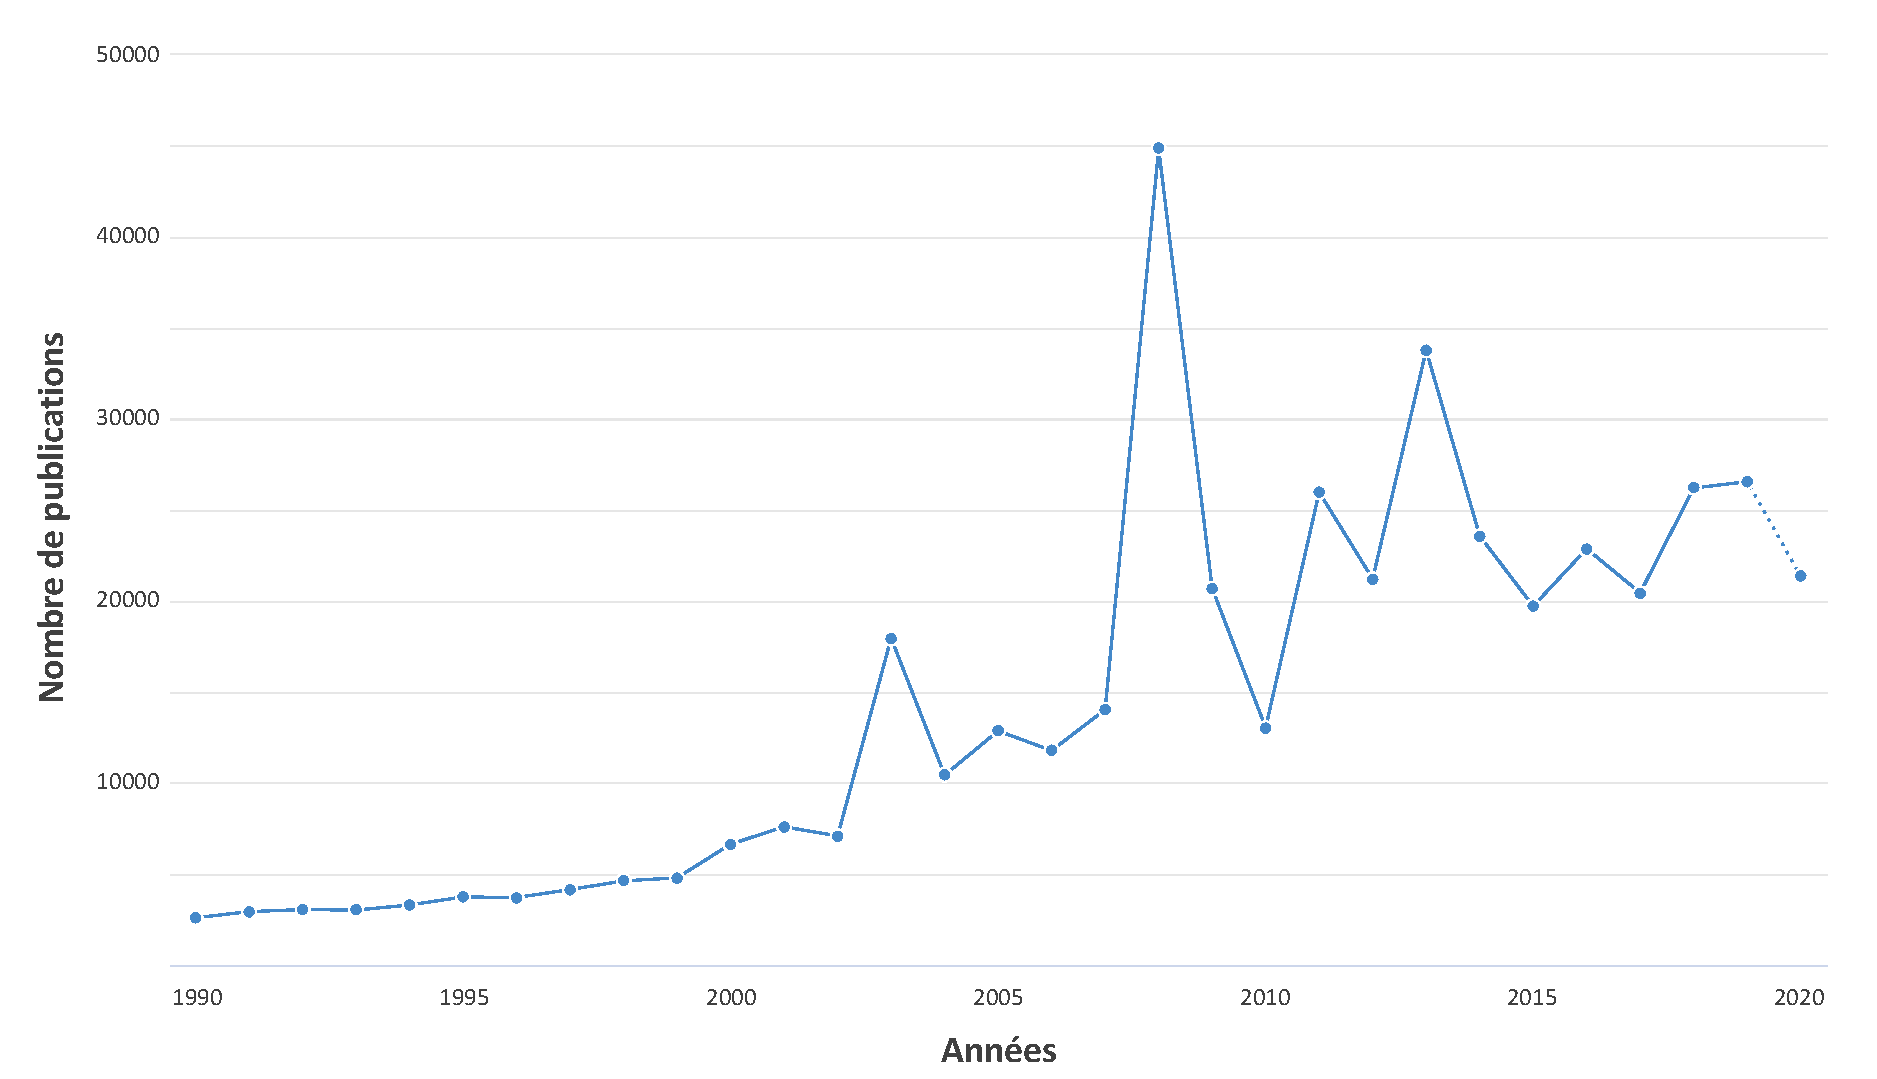
\includegraphics[width=\linewidth]{contents/i_introduction/resources/evolution_publications.pdf}
    \caption{Graphique représentant l'évolution du nombre de publications recensées par le moteur de recherche \href{https://scholar.google.fr/}{Google Scholar}~\textsuperscript{\ref{footnote:evolution_publications}} autour des termes de « skin computer diagnosis » entre les années 1990 et 2020.}
    \label{fig:evolution_publications}
\end{figure}\par
\addtocounter{footnote}{1}
\footnotetext[\thefootnote]{Source image~:~Graphique généré à partir du site \href{https://www.dimensions.ai/}{Dimensions.}  \label{footnote:evolution_publications}}

La matière première mise à la disposition de ce travail permet une orientation de ces travaux dans le sens de la multimodalité. En effet, l'une des problématiques majeures aujourd'hui en dermatologie est ce que les médecins qualifient de zone d'indécision, également appelée \textit{zone grise}. Il s'agit d'une catégorie de cas cliniques pour lesquels le médecin n'a pas à un instant $t$ suffisamment d'informations ou de connaissances pour prendre une décision. Ces cas nécessitent souvent une prise en charge plus importante, avec l'aide d'autres spécialistes ou encore avec notamment de nouveaux examens plus spécifiques.\par

La finalité de ce travail est de proposer diverses méthodes et outils permettant une aide à la décision dans la gestion de cette zone grise, et ainsi améliorer la prise en charge clinique en service de dermatologie. À l'instar des travaux existants, cette gestion de la zone grise passe d'une part par l'implémentation de méthodes propres à certaines des modalités de ce travail et d'autre part par la mise en place d'un schéma multimodal. Ainsi, un schéma résumant ce l'objectif de ce processus est visible sur la \Cref{fig:scheme_reduce_indecision}.\par
\clearpage

Dans ce schéma idéal représenté sur la \Cref{fig:scheme_reduce_indecision}, les patients jugés avec une certaine certitude comme \textbf{bénins} ou \textbf{malins}, seront exclus des procédures suivantes. Seuls les patients encore présents dans cette \textit{zone grise} sont pris en charge pour des examens supplémentaires, pour lesquels ce processus est réitéré.\par 

\begin{figure}[H]
    \centering
    \includegraphics[width=\linewidth]{contents/i_introduction/resources/scheme_reduce_indecision.pdf}
    \caption{Schéma de représentation du processus de réduction de l'indécision, également surnommée zone grise. Ce travail s'inspire du processus cognitif des dermatologues et consiste à réduire l'indécision propre à chacune des modalités clinique par l'ajout de nouvelles modalités d'imagerie.}
    \label{fig:scheme_reduce_indecision}
\end{figure}\par

À cette fin, ce travail mobilise des connaissances en provenance de divers champs d'applications propres~:
\begin{inlinerate}
    \item à la peau d'un point de vue médical, 
    \item aux modalités permettant l'observation des tissus,
    \item et à l'intelligence artificielle.
\end{inlinerate} Cette complémentarité est représentée sous forme de schéma sur la \Cref{fig:scheme_our_work}.\par

\begin{figure}[H]
    \centering
    \includegraphics[width=0.8\linewidth]{contents/i_introduction/resources/scheme_our_work.pdf}
    \caption{Schéma de représentation des divers domaines impliqués dans cette thématique de recherche. Ce travail est au confluent de connaissances de la peau, des modalités d'imagerie et des domaines de l'intelligence artificielle.}
    \label{fig:scheme_our_work}
\end{figure}\par

Dans un premier temps, le contexte de cette étude est abordé dans la \Cref{part:contexte}. Cette partie débute par une présentation de la peau, l'organe majeur de cette étude, réalisée au sein du \Cref{chap:chapter_1}. Puis, s'ensuit une mise en évidence des principes d'interaction entre la peau et la lumière, avant de présenter les techniques de visualisation à la disposition des médecins dans le \Cref{chap:chapter_2}. Ensuite, le \Cref{chap:chapter_3} présente au lecteur l'ensemble des connaissances d'intelligence artificielle sollicitées dans ce manuscrit. Pour finir cette partie, le \Cref{chap:chapter_4} présente les données mises à disposition de cette étude mais également les principaux travaux en lien avec ce travail.\par

Dans un second temps, la prise en charge de la modalité de \gls{mcr} est abordé par la \Cref{part:microscopy}. À cette fin, cette partie débute par le traitement des images de cette modalité dans le \Cref{chap:chapter_5} dédié à la classification de ces images et propose une extension de ces travaux dans le \Cref{chap:chapter_6}. Pour finir, le \Cref{chap:chapter_7} propose diverses méthodes permettant à partir des images de remonter à la prise de décision au niveau d'une lésion.\par

Dans un dernier temps, la finalité de ce travail est traitée par la \Cref{part:multimodal} dédiée à l'apport de l'information multimodale. Dans ce but, le \Cref{chap:chapter_8} reprend les observations de travaux sur les modalités d'imagerie clinique et de dermatoscopie ainsi que celles issues de la précédente partie sur la modalité de \gls{mcr}, et propose des méthodes d'agrégation séquentielles de ces informations.\par

Dans la mesure où certains termes d'origine anglaise ne possèdent pas de réel équivalent dans la langue française, ce travail favorise l'utilisation d'acronymes français pour les termes communément acceptés tels que les \textit{modalités d'imagerie} ou encore les \textit{pathologies de la peau}. En revanche, par souci d'homogénéité les \textit{termes techniques sont proposés en anglais} bien que certains aient trouvé leur équivalent dans la langue française. Quel que soit l’acronyme employé, ce travail propose à la première utilisation un format du type~:~\textbf{Langue Cible, LC (alternative~:~Langue Alternative, LA)}.\par

% Part 1
\part{Contexte}
\label{part:contexte}
\renewcommand{\thechapter}{\roman{chapter}}
\setcounter{chapter}{2}

\unchapter{Préambule contexte}
\label{chap:preamble_context}

Ce travail va s'inscrire dans une démarche d'aide au diagnostic des lésions de la peau et particulièrement des pathologies de \glsfirst{lm} et \glsfirst{lmm}. De nombreux travaux se sont portés sur l'aide à la détection par ordinateur de lésions de la peau similaires, à l'aide de modalités unique d'imagerie. Néanmoins, peu d'entre eux s'intéressent à une démarche multimodale de cette thématique, soit par non considération de cette application, soit par un manque suffisant de données à leur disposition.\par

La matière première mise à notre disposition permettra une orientation de nos travaux dans le sens de la multimodalité. En effet, l'une des problématique majeure aujourd'hui en dermatologie, est ce que les médecins qualifient de zone d'indécision, également appelée \textit{zone grise}. Il s'agit d'une catégorie de cas cliniques pour lesquels le médecin n'a pas à un instant $t$ suffisamment d'information en sa possession ou les connaissances suffisantes pour prendre une décision. Ces cas nécessitent souvent une prise en charge plus importante, avec l'aide d'autres spécialistes ou encore avec notamment de nouveaux examens plus spécifiques.\par

Nous souhaitons par ce travail, amener diverses techniques et outils permettant une aide à la décision dans la gestion de cette zone grise, et ainsi améliorer la condition clinique en service de dermatologie. Ainsi, nous proposons un schéma macroscopique de cet objectif en \Cref{fig:scheme_reduce_indecision}.\par

\begin{figure}[H]
    \centering
    \includegraphics[width=\linewidth]{contents/ii_preamble_context/resources/scheme_reduce_indecision.pdf}
    \caption{Représentation du processus de réduction de l'indécision du médecin ou \textit{zone grise}. Ainsi, ce travail à pour objectif de réduire par l'apport de nouvelles modalités les divers cas portant à confusion de manière similaire au processus congnitif des dermatologues.}
    \label{fig:scheme_reduce_indecision}
\end{figure}\par

A cette fin, nous mobiliserons des connaissances en provenance propre à la peau, aux modalités d'observation et à l'intelligence artificielle, tel que représenté en \Cref{fig:scheme_our_work}. Pour cela, nous mettrons à disposition du lecteur l'ensemble des bases nécessaire à la compréhension de ce sujet au travers de cette partie de contexte. Nous débuterons au sein du \Cref{chap:chapter_1} par une présentation de la peau, c'est à dire l'organe majeure de cette étude. Puis, nous procéderons à l'aide du \Cref{chap:chapter_2} à une mise en évidence des principes d'interaction entre la peau et la lumière, avant de présenter les techniques de visualisations mises à disposition des médecins. Pour finir cette partie, nous réaliserons un descriptif des méthodes d'intelligence artificielle applicable à ce travail.\par

\begin{figure}[H]
    \centering
    \includegraphics[width=\linewidth]{contents/ii_preamble_context/resources/scheme_our_work.pdf}
    \caption{Macro représentation des domaines impliqués de cette thématique de recherche. Notre travail se retrouve ainsi au confluents de connaissance de la peau, des modalités d'imagerie permettant son acquisition et des domaines de l'intelligence artificielle.}
    \label{fig:scheme_our_work}
\end{figure}\par
\chapter{La peau}
\label{chap:chapter_1}
Le terme "peau" caractérise dans son sens le plus global, l’enveloppe externe propre aux vertébrés. Présente chez l’homme, elle est l’un de ses organes majeurs mais également l’un des plus lourds : chez un individu adulte d’un poids de \SI{70}{\kilo\gram}, elle représente une surface plane d’environ \SI{2}{\metre\squared}, soit une masse estimée à \SI{5}{\kilo\gram} \cite{McGrath2010}. Son épaisseur diffère selon la zone du corps étudiée : de \SI{0,5}{\milli\metre} au niveau de zones fines telles que les paupières, à \SI{5}{\milli\metre} sur des zones plus épaisses tel que le haut du dos. Cet organe souvent méconnu, voire oublié par la plupart d’entre nous, assure pourtant des fonctionnalités multiples : 
\begin{itemize}
\item La protection contre le monde extérieur
\item La limitation de la perte d’eau
\item La thermorégulation
\item L’appréhension physique de notre monde
\item \ldots
\end{itemize}\par
La dermatologie, branche médicale vouée à l’étude de la peau, nous permet de mieux comprendre sa composition, son fonctionnement, ses vulnérabilités et permet d’apporter conseils, préventions et traitements dans le cas de certaines pathologies.\par
Cette barrière se décompose en diverses couches fondamentales : l’épiderme, la membrane basale, le derme et l’hypoderme, dont la représentation est visible au travers de la \Cref{fig:skin_kholoski}.\par
\begin{figure}[H]
    \centering
    \includegraphics[width=0.6\linewidth]{contents/chapter_1/resources/skin_kholoski.png}
    \caption{Représentation macroscopique de la peau \textsuperscript{\ref{footnote:skin_kholoski}}.}
    \label{fig:skin_kholoski}
\end{figure}
\addtocounter{footnote}{1}
\footnotetext[\thefootnote]{Image source : Dessin par \href{http://kholoski.com/}{Kellie Holoski} – Illustrateur médical. \label{footnote:skin_kholoski}}
\clearpage

\section{Compositions et fonctions}
Avant d’aborder les lésions pouvant affecter cet organe, nous allons introduire de manière synthétique sa composition et son fonctionnement. Nous étudierons chaque couche évoquée par ordre de profondeur croissante.\par

\subsection{Épiderme}
L’épiderme correspond à la couche superficielle de notre peau et mesure entre \SI{0,01}{\milli\metre} et \SI{0,1}{\milli\metre} d’épaisseur \cite{Sandby-Moller2003}. Un aperçu des différents types de cellules la composant peut être visible sur la \Cref{fig:epidermis_kholoski}, parmi lesquelles :
\begin{itemize}
\item Kératinocytes : 90 \% des cellules, rôle de protection
\item Cellules de Langerhans : cellules immunitaires
\item Cellules de Merkel : cellules sensitives
\item Mélanocytes : cellules de protection contre les \gls{uv}.
\end{itemize}\par

 \begin{figure}[H]
    \centering
    \includegraphics[width=0.7\linewidth]{contents/chapter_1/resources/epidermis_kholoski.png}
    \caption{Schématisation de la composition de l’épiderme \textsuperscript{\ref{footnote:epidermis_kholoski}}.}
    \label{fig:epidermis_kholoski}
\end{figure}\par

\addtocounter{footnote}{1}
\footnotetext[\thefootnote]{Image source : Dessin par \href{http://kholoski.com/}{Kellie Holoski} – Illustrateur médical. \label{footnote:epidermis_kholoski}}

Son processus de différenciation des cellules est l’une de ses caractéristiques essentielles. Les kératinocytes, sa principale composante, migrent de la couche inférieure à la couche supérieure en subissant différentes modifications chimiques conduisant à la perte de leur noyau et à la mort de ces cellules. Ce processus porte le nom de kératinisation, et se subdivise en sous couches aux propriétés variées, respectivement par profondeur croissante : Cornée (Stratum corneum), Transition (Stratum lucidum), Granuleuse (Stratum granulosum), Epineuse (Stratum spinosum), Basale (Stratum basale). Ces différentes couches peuvent être observées en \Cref{fig:epidermis_kholoski}. En fin de parcours, ces cellules perdent leur cohésion dans un processus de desquamation conduisant la peau à se renouveler.\par\clearpage

\subsection{Membrane basale}
La membrane basale se situe à la jonction de l’épiderme et du derme (ou jonction dermo-épidermique), et peut être observée par microscopie optique ou électronique selon l’épaisseur de cette dernière. Son épaisseur, variable selon la zone considérée, est estimée entre \SI{60}{\nano\metre} et \SI{300}{\nano\metre}. 
Cette membrane est scindée en 2 parties :
\begin{itemize}
\item La lame basale (lamina basalis), divisée en deux couches : Lamina Lucida et Lamina Densa
\item La lame réticulaire ou zone fibrillaire (lamina reticularis ou fibroreticularis).
\end{itemize}\par
\begin{figure}[H]
    \centering
    \includegraphics[width=\linewidth]{contents/chapter_1/resources/basal_basement.pdf}
    \caption{Schématisation macroscopique de la membrane basale \textsuperscript{\ref{footnote:basal_basement}}.}
    \label{fig:basal_basement}
\end{figure}\par

\addtocounter{footnote}{1}
\footnotetext[\thefootnote]{Image source : Principles of Anatomy and Physiology – John Wiley \& Sons. \label{footnote:basal_basement}}

Il s’agit d’une zone fibreuse, composée de laminine, de collagène de type III / IV / VI lui conférant entre autres des propriétés de résistance mécanique, voire élastiques. Ces fibres lui permettent d’assurer une cohésion entre épiderme et derme au travers de points d’ancrage. Sa seconde fonction essentielle est au travers d’un mécanisme de régulation des échanges moléculaires, permettant d’assurer la nutrition des cellules de base de l’épiderme. Pour finir, elle possède un rôle de ré épidermisation fondamentale lors de la cicatrisation.\par
\clearpage

\subsection{Derme}
Le derme est une couche d’une épaisseur estimée comprise entre \SI{0,5}{\milli\metre} et \SI{5}{\milli\metre}, composée majoritairement de collagène à hauteur de 80 \% (sur la matières sèche), et de fibres élastiques \cite{McGrath2010}. Cette couche est traversée par de nombreux éléments dont : 

\begin{itemize}
\item Des vaisseaux sanguins, qui apportent nutriments
\item Des vaisseaux lymphatiques, qui assurent une fonction immunitaire.
\end{itemize}\par

En outre, cette strate contribue de manière essentielle à des aspects de résistance et contrainte mécanique de la peau, ainsi qu’aux mécanismes de thermorégulation et de cicatrisation de cette dernière. Enfin, cette couche tient un rôle essentiel dans la perception sensorielle (somesthésie) assurant d’une part des propriétés liées à la pression (mécanorécepteurs) mais également liées à la chaleur (thermorécepteurs). Outre ces fonctions, on lui attribue également un rôle nutritif important de par son irrigation sanguine.\par
La littérature identifie deux parties majeures au sein du derme. Celles si sont visibles en \Cref{fig:dermis_kholoski}, nous retrouvons:
\begin{itemize}
\item Le derme Papillaire (Papillary dermis), permettant essentiellement la thermorégulation
\item Le derme Réticulaire (Reticular dermis), assurant la plupart des fonctions mécaniques.
\end{itemize}\par

\begin{figure}[H]
    \centering
    \includegraphics[width=\linewidth]{contents/chapter_1/resources/dermis_kholoski.pdf}
    \caption{Schéma d’approche du derme \textsuperscript{\ref{footnote:dermis_kholoski}}.}
    \label{fig:dermis_kholoski}
\end{figure}\par

\addtocounter{footnote}{1}
\footnotetext[\thefootnote]{Image source : Dessin par \href{http://kholoski.com/}{Kellie Holoski} – Illustrateur médical. \label{footnote:dermis_kholoski}}
\clearpage

\subsection{Hypoderme}
L’hypoderme, également appelée couche sous cutanée, est un tissu présent sous le derme composé essentiellement de graisses (adipocytes, cellules spécialisées dans le stockage de graisses). Son épaisseur est extrêmement variable de \SI{0,1}{\centi\metre} à \SI[parse-numbers = false]{plusieurs}{\centi\metre}, selon :
\begin{itemize}
\item La zone considérée
\item L’âge du patient
\item L’alimentation
\item Les prédispositions génétiques.
\end{itemize}\par

Cette couche de tissu assure diverses fonctions, dont :
\begin{itemize}
\item Le passage des vaisseaux sanguins et lymphatiques, ainsi que des nerfs jusqu’au derme
\item L’interface entre les structures sous cutanées et la peau.
\end{itemize}\par

\subsection{Types de peau}
Il est nécessaire afin de bien aborder ce sujet et ses problématiques, d’être conscient des variations inter individus. Pour répondre partiellement à ces variations, Fitzpatrick T. a établi une classification des profils type de peau, visant à caractériser leur réaction suite à l’exposition au soleil. Ce travail a également permis de créer une association entre profil type et couleur de peau avant et après exposition au soleil \cite{Fitzpatrick1988}. 
\begin{figure}[H]
    \centering
    \includegraphics[width=\linewidth]{contents/chapter_1/resources/Fitzpatrick.pdf}
    \caption{Échelle de Fitzpatrick associant type de peau et caractéristiques associées \cite{Fitzpatrick1988}.}
    \label{fig:fitzpatrick}
\end{figure}
Cet aspect est un élément important à prendre en compte lors de notre appréhension de la problématique. En effet, la littérature semble majoritairement axée sur les types I/II de peau, certaines pathologies seront ainsi plus propices à certaines peaux \cite{Narayanan2010}. De plus, une même pathologie pourra diverger en terme de caractéristiques \cite{Tuma2015}. Nous retrouvons en \Cref{fig:fitzpatrick}, une synthèse visuelle de ces types de peau et de leurs caractéristiques.

\section{Lésions de la peau}
Notre sujet abordant les lésions de la peau, il convient de définir le terme lésion pour bien situer l’objet de notre recherche. Selon PubMed, une lésion « correspond à toute anomalie touchant les tissus d’un organisme, généralement provoqué par une maladie ou par un traumatisme. » \textsuperscript{\ref{footnote:lesion_pubmed}}.\par
\addtocounter{footnote}{1}
\footnotetext[\thefootnote]{Source : Définition par \href{https://www.ncbi.nlm.nih.gov/pubmedhealth}{PubMed Health}. \label{footnote:lesion_pubmed}}

Les lésions de la peau correspondent à un terme générique caractérisant une partie de la peau ayant, en comparaison de la peau l’entourant, une croissance/apparence ou structure qui diffère. Ces lésions peuvent être pré ou post natal, comporter diverses formes et peuvent présenter différents risques.\par
Nous décrivons par le terme « lésion pigmentaires », les lésions affectant la peau présentant des pigmentations liées à la mélanine, au sang, ou de tout autre composant extérieur à la peau. Ces lésions peuvent être d’origine mélanocytaire (Nævus mélanocytaires) ou non mélanocytaire (nous nous intéresserons aux divers carcinomes lorsque nous aborderons les lésions malignes).\par
Nous traiterons sommairement des lésions de la peau au travers de ces quelques pages. Nous aborderons dans un premier temps des lésions bénignes et nous orienterons dans un second temps ce travail vers les lésions dites malignes. Enfin, nous présenterons le Lentigo, pathologie que nous étudierons dans ce manuscrit.\par

\subsection{Lésions bénignes}
Ces lésions désignent les diverses altérations classées comme sans gravité pour la santé. Néanmoins ces lésions peuvent présenter un terrain pour des lésions plus dangereuses.\par
L'une des lésions bénigne les plus communes est le Naevus mélanocytaire souvent associé au « grain de beauté », a l’apparence de structures souvent circulaires ou ovales présentent en surface de peau chez l’homme. Les naevus sont susceptibles d’évoluer au cours du temps et peuvent dans très peu de cas aboutir à un mélanome. Ces tâches apparaissent durant les trente premières années de vie en moyenne et présentent des couleurs variées : de teintes allant vers le jaune à des bruns foncés. Voici quelques-unes des catégories et critères associés :
\begin{itemize}
\item Nævus commun, ou « grain de beauté » est le plus fréquent et se compose de mélanocytes regroupés en amas
\item Nævus atypique, se caractérise la plupart du temps par une pigmentation variable et des bordures irrégulières
\item Nævus congénital, apparaît en début de vie, peut apparaître sous forme de tâche
\item Nævus de Spitz, s’apparente souvent à un mélanome de part diverses caractéristiques. On y observe une croissance rapide en 2 à 6 mois ainsi qu’une couleur brun-rouge
\item Phénomène de Sutton, dé-pigmentation aux abords d’un naevus existant sur une durée de quelques semaines à quelques mois. Chez l’adulte, ce phénomène peut être un signe de mélanome.
\end{itemize}
Il convient de réaliser un surveillance régulière de ces lésions bénignes au sens large, afin de s'assurer qu'elle ne dégénère pas en pathologie maligne.\par

\subsection{Lésions malignes}
Avant de débuter, commençons par caractériser le terme malin, signifiant dans notre contexte « une maladie grave ou une tumeur pouvant se généraliser et entraîner la mort ». Nous traiterons au travers de cette partie des pathologies majeures, sujettes à entraîner le décès d’un individu. Ce décès est souvent la résultante de pathologie dites cancéreuse, c'est à dire « qui pour la plupart colonise les tissus alentours, susceptible de réapparaître après une tentative de retrait et de tuer le patient à moins d’être traité de manière adéquate ». Les cancers de la peau sont issus d’une division ou d’une mutation anormale de cellules de la peau et, résultent pour la plupart d’une exposition aux \gls{uv}, principal facteur de mutation. D’autres facteurs tels que le tabagisme, les virus, des prédispositions génétiques ou encore l’utilisation de médicaments immunosuppresseurs peuvent favoriser leur apparition. Les quelques sous parties suivantes donne un aperçu des pathologies malignes majeures.\par

\subsubsection{Mélanome}
Le mélanome est une forme de cancer de la peau, se développant à partir de mélanocytes, également qualifié de tumeur mélanocytaire. Ce type de cancer se développe dans environ 70 \% des cas sur une peau saine et dans les 30 \% restants sur un naevus présent au préalable. Cette anomalie représente 2 \% des cas de cancers de la peau \cite{TortoraG;Derrickson2012}. Néanmoins, en contrepartie il s’agit de la forme la plus mortelle de cancer de la peau, avec au niveau mondial, une incidence de 350 000 cas en 2015. Ce cancer est par ailleurs responsable d’environ 59 800 décès \cite{Karimkhani2017}. Son incidence est fortement aggravée par l’exposition prolongée au soleil et plus particulièrement aux \gls{uv}. Les types I/II sur l’échelle de Fitzpatrick sont également les plus ciblés en proportion.
Comme pour les naevus, plusieurs types de mélanomes sont recensés, séparés en deux groupes distincts. D’une part les pathologies superficielles caractérisent les mélanomes présentant une phase d’extension épidermique (extension horizontale) suivi par une phase de développement en profondeur (extension verticale). Cette catégorie se compose de :
\begin{itemize}
\item Mélanomes d'extension superficielle – environ 70 \% des mélanomes
\item Mélanomes de Dubreuilh – environ 10 \% des mélanomes \cite{LeGal2011}
\item Mélanomes acro-lentigineux – environ 10 \% des mélanomes.
\end{itemize}
\begin{figure}[H]
    \centering
    \includegraphics[width=0.7\linewidth]{contents/chapter_1/resources/clarklevels_kholoski.png}
    \caption{Illustration des différents niveau de Clark \cite{Clark1969} \textsuperscript{\ref{footnote:clarklevels_kholoski}}.}
    \label{fig:clarklevels_kholoski}
\end{figure}\par
\addtocounter{footnote}{1}
\footnotetext[\thefootnote]{Image source : Dessin par \href{http://kholoski.com/}{Kellie Holoski} – Illustrateur médical. \label{footnote:clarklevels_kholoski}}
La seconde catégorie se compose des mélanomes nodulaires. Ceux-ci, se démarquent par une évolution plus rapide. En effet, dans une majeure partie, ceux-ci se développent verticalement dès les premiers symptômes. Une échelle, connue sous le nom de niveau de Clark (\Cref{fig:clarklevels_kholoski}), a été définie dans le but de caractériser le stade d’un mélanome \cite{Clark1969}.\par

\subsubsection{Cancer épidermoïde ou spinocellulaire}
Les cancers épidermoïdes ou spinocellulaires de la peau, prennent racine au niveau des épithéliums de l’épiderme dont la croissance devient incontrôlée. L’apparence de cette pathologie est diverse, variant de simples plaques rouges à des cas de plaies ouvertes. Cette pathologie est plus à même de provoquer des métastases chez un individu, et donc de se propager. 
Ce type de cancer est au second rang des cancers cutanés les plus graves, principalement lié à cette caractéristique de propagation. Ces cancers émergent le plus souvent de zones exposées régulièrement au soleil telles que le visage, les oreilles, le cou, etc… Ces zones exposées dénotent souvent de nombreux symptômes liés au dommage du soleil :
\begin{itemize}
\item Rides
\item Perte d’élasticité
\item Tâches
\end{itemize}
Les prédispositions génétiques, les conditions de travail et le sexe d’un individu sont autant de facteur pouvant influer sur l’apparition de ce type de cancer.\par

\subsubsection{Carcinome basocellulaire}	
Le carcinome basocellulaire correspond à une surcroissance de cellules de l’épiderme, plus précisément de ses cellules basales. Il s’agit d’une des formes de cancer de la peau la plus commune, ses conséquences médicales sont par oppositions moindres. En effet, ces cancers ont peu de risque de métastases et sont donc moins enclins à se propager à l’ensemble de l’organisme, et de provoquer la mort du patient. Ce cancer peut résulter de divers facteurs comme ses homologues, dont les principaux restent la surexposition au soleil ou la défaillance du système immunitaire.\par

\subsection{Une pathologie particulière: le Lentigo maligna}
Le terme \gls{lm} et \gls{lmm} sont des alternative anglo-saxonne largement acceptées des termes francophone mélanome de Dubreuilh et mélanome sur mélanome de Dubreuilh qui touche les zones les plus exposées tel que le visage chez les populations âgées Comme précédemment énoncé, ils représentent environ 10\% des cas de mélanome mais tend à augmenter ces dernières années avec une exposition au soleil croissante et va jusqu'à toucher les populations considérées comme jeunes. Des études moléculaires et épidémiologiques tendent à distinguer deux principaux mode de développement de ces pathologies: l'une chez le sujet jeune, ayant de nombreux nævi et ayant une exposition solaire intermittente mais intense et l'autre chez le sujet plus âgée ayant été chroniquement été exposé au soleil \cite{LeGal2011}.\par
Le \gls{lm} est la résultante d'une prolifération de cellules au sein de la couche basale de l'épiderme, considéré par certains spécialistes comme melanoma-in-situ ou stade 0. Lorsque cette prolifération se propage aux couches inférieures par le biais des follicules pileux, nous parlons de \gls{lmm}. A l’œil nu, ces pathologies sont difficiles à distinguer de pathologies bénignes telles qu'un lentigo solaire, une kératose actinique pigmentée ou une kératose séborrhéique \cite{LeGal2011}.\par
Le \gls{lm} et \gls{lmm} se caractérise souvent par des macules pigmentées, des bordure et pigmentation irrégulières. Par ailleurs, ces pathologies touche majoritairement les personnes de plus de 60 ans et des zones exposées telles que le visage ou le dos des mains.\par
Le diagnostic considéré comme "gold standard" ou test de référence à ce jour est l'histopathologie. C'est à dire que le médecin procède à l'excision d'un tissu considéré comme pathologique (ou biopsie), puis ce même tissu est préparé afin d'être observé par microscope pour procédé à une analyse histologique. Ce type de procédure est relativement coûteux en temps, et représente une ressource financière importante si l'on considère le coût par patient. De plus, il s'agit d'une procédure incommodante pour le patient. De plus, une analyse peut échouer si le prélèvement est effectué en dehors de la zone pathologique \cite{LeGal2011}.\par
Les nombreuses contraintes actuelles liées aux coûts, à l'augmentation des patients et au respect du patient oriente vers des techniques non invasives plus rapide à mettre en oeuvre. Le chapitre suivant s'oriente en ce sens en apportant des bases quand au propriété phyisique de la peau et à la manière de l'observer.\par 
%%%%% CHAPTER SKIN PROPERTIES TO DATA
% \chapter{De propriété physiques de la peau aux données de travail}
\chapter{Des propriétés physiques aux données cliniques}
\label{chap:chapter_2}
\chapterintro
Lors du précédent chapitre, nous avons pu présenter la peau, ses pathologies dont l'une d'entre elle en particulier: le Lentigo Maligna et le Lentigo Maligna Melanoma. Nous avons également pu présenter les moyens actuels permettant son diagnostic et ses contraintes actuelles.\par
Ce nouveau nouveau chapitre nous permet d'appréhender certaines propriétés physiques de la peau, notamment les mécanismes d'interaction avec la lumière. Dans un second temps, ce chapitre évoque les principaux dispositifs optiques actuels et le type d'information mise à disposition pouvant servir le diagnostic, mais également certains dispositifs actuellement considéré pour la dermatologie basés sur des mesures physique autres.\par
Pour finir, ce chapitre servira à présenter nous permet de présenter l'étude clinique ayant servie de base à ce travail et de comprendre sa construction. Nous présenterons également la base d'image permettant la réalisation de nos divers tests.\par 
\newpage

% SECTION SKIN PROPERTIES
\section{Propriétés de la peau}
Notre perception de la peau est façonnés par divers phénomènes physique d'interaction entre la lumière et ses tissus. Ces derniers influent: 
\begin{inlinerate}
\item de par leur structure 
\item et de par leur composantes.
\end{inlinerate}
Nous aborderons cette section de manière descendante, en déroulant le processus d'interaction d'un photon qui entre en contact avec la peau. Ce processus est schématisé de manière macroscopique en \Cref{fig:light_interaction}. La réflexion spéculaire est le premier phénomène pouvant se produire, à l'interface air/peau et est due au changement d'indice de réfraction. Ce faisant, la partie résiduelle parvenue à la peau va interagir avec les diverses structures de la peau et être soit ré émise sans modification de longueur d'onde, nous parlons alors de réflexion diffuse, soit absorbé, nous parlons dans ce cas d'absorption. Cette absorption peut réagir de diverses manière selon la nature du composé et selon la longueur d'onde de l'énergie reçue: 
\begin{inlinerate}
\item l'énergie peut-être dissipé sous forme de chaleur
\item ou être ré émise avec longueur d'onde différente souvent caractérisé par le terme de fluorescence~\cite{Kollias2002}.
\end{inlinerate}\par

\begin{figure}[H]
    \centering
    \includegraphics[width=\linewidth]{contents/chapter_2/resources/light_interaction.pdf}
    \caption{Mécanismes d'interaction primaire avec un photon incident.}
    \label{fig:light_interaction}
\end{figure}\par

Dans cette configuration, le choix de la source d'émission de lumière sera l'un des points importants. En effet, comme démontré dans un travail précédent sur les \gls{led} en dermatologie~\cite{Barolet2008}, la longueur d'onde d'émission est l'un des paramètre d'influence possible quand à la profondeur des structures à observer dans la peau. Ainsi, des longueurs d'onde à l'entrée du spectre visible humain ($\approx$\SI{300}{\nano\metre}) ne parviennent pas à se frayer un chemin en profondeur et ne frôlent que les couches supérieures de l'épiderme, tandis que des longueur d'ondes plus élevée de ce même spectre ($\approx$\SI{900}{\nano\metre}) tendent à atteindre l'hypoderme et ses vaisseaux sanguins. Une synthèse de la pénétration de la lumière en fonction de la longueur d'onde est visible en \Cref{fig:light_penatrating}.\par

\begin{figure}[H]
    \centering
    \includegraphics[width=0.8\linewidth]{contents/chapter_2/resources/light_penatrating.png}
    \caption{Schéma représentatif des longueurs d’onde et de leur capacité de pénétration de la peau \cite{Barolet2008}.}
    \label{fig:light_penatrating}
\end{figure}\par

Outre la question de la profondeur, le choix de la longueur d'onde permet d'interagir avec différents types de chromophores pouvant renseigner l'observateur sur des propriétés locales à la peau. Certains travaux focalisés sur les systèmes lasers et d'émission en général~\cite{Stewart2013} ont permis de mettre en avant le rapport entre la longueur d'onde et des composés majeurs de la peau tels que l'eau, la mélanine ou l'hémoglobine (oxygénée ou non). Pour illustrer ce propos, la \Cref{fig:light_absorption} synthétise ce rapport entre la longueur d'onde d'émission et l'absorption associée à ces quatre composés. La quantification de ces composés peut présenter un intérêt dans la mesure où certaines pathologie peuvent altérer le métabolisme et donc modifier fondamentalement le ratio de chromophores présents, pouvant par exemple amener à une hypervascularisation. Certains travaux tentent ainsi de revenir à des fonctions de métabolisme~\cite{Im2016}.\par

\begin{figure}[H]
    \centering
    \includegraphics[width=\linewidth]{contents/chapter_2/resources/light_absorption.png}
    \caption{Représentation des longueurs d'ondes et coefficients d'absorption associé selon le type de composé \cite{Stewart2013}.}
    \label{fig:light_absorption}
\end{figure}
 
\clearpage
\section{Modalités d’imagerie non invasives}
Afin de mieux suivre, voire de conserver une trace de leurs patients, les dermatologues disposent de nombreux outils divers. Ils peuvent entre autres dans leur pratique clinique se référer à divers types d’examen que nous distinguerons au travers de deux catégories :
\begin{itemize}
\item D’une part les examens invasifs, pouvant altérer l’organisme du patient à plus ou moins grande échelle. La biopsie est à ce jour le « gold standard » de ce domaine et se réalise par prélèvement et analyse des tissus du patient. Ces techniques sont généralement plus coûteuses à réaliser par unité, nécessitent davantage de temps et peuvent engendrer une gêne voire un risque lors de leur exécution.
\item D’autres part, les examens dit non invasifs, c’est-à-dire ne provoquant pas d’effraction des tissus de la peau parmi lesquels les « imageurs », dispositifs capables de nous restituer une image de différente nature selon le phénomène physique observé. Les coûts peuvent être plus ou moins élevées selon le type de dispositif utilisé et ne procurent en général pas d’inconfort particulier pour la plupart.
\end{itemize}\par

Après avoir abordé de manière non exhaustive les majeures pathologies de la peau et quelques principes d'interaction avec la peau, il convient désormais d'aborder les diverses méthodes permettant une observation non invasives. Ces modalités d'imagerie franchissent en majorité le cap du numérique permettant un suivi plus aisé, voire un échange plus rapide entre professionnels, et l’utilisation de traitements automatiques. Nous séparerons ces techniques en deux catégories distinctes: d’une part les techniques de mesure optique et d'autres part les autres dispositifs basées sur une mesures physique indépendante de l'optique.\par

\subsection{Modalités par mesure optique}
\begin{table}[H]
\begin{tabular}{lllll}
\textbf{Technologie}                                                                & \textbf{Mode d’émission} & \textbf{Résolution Spatiale} & \textbf{Profondeur}                   \\ \hline
Imagerie clinique                                                                   & Réflectance              & Lentille dépendant           & \SIrange{0.1}{1}{\milli\metre}        \\
Dermatoscope                                                                        & Réflectance              & Lentille dépendant           & \SIrange{0.1}{1}{\milli\metre}        \\
Microscope confocale par réflectance                                                & Réflectance              & \si{\micro\metre}            & \textless{} \SI{200}{\micro\metre}    \\
Tomographie en cohérence optique                                                    & Réflectance              & \si{\micro\metre}            & \SIrange{1}{2}{\milli\metre}          \\
Imagerie multispectrale                                                             & Réflectance              & Lentille dépendant           & \SIrange{0.1}{1}{\milli\metre}        \\
Spectroscopie à réflexion/fluorescence                                              & Réflectance/Fluorescence & Diamètre de la fibre         & \SIrange{0.1}{1}{\milli\metre}        \\
Microscopie confocal Raman                                                           & Raman                    & \si{\micro\metre}            & \SI{150}{\milli\metre}                \\
% Réflectance totale atténuée                                                         & ATR                      & Dimension du Crystal         & \textless{} \SI{2}{\micro\metre}      \\
\end{tabular}
\caption{Aperçu des principales modalités de mesure optique actuelles en dermatologie utilisées cliniquement ou expérimetalement \cite{Kollias2002}.}
\label{tab:light_absorption}
\end{table}\par

\subsubsection{Imagerie clinique}
L’examen de dépistage classique est associé en dermatologie à une inspection à l’œil nu exercée par une personne compétente ou sensibilisée à la détection de pathologies. Cette première modalité fait appel à un dispositif de photographie non propre à la dermatologie. Par ailleurs, n’étant pas spécifique à ce domaine, elle constitue la modalité la moins onéreuse de la discipline dans le cadre de l’imagerie des lésions.\par

Cette modalité, avant l’avènement de l’informatique, se basait sur des supports de type argentique. L’évolution de ce matériel vers le numérique, et l’arrivée de systèmes de type \gls{pacs} ont conjointement motivé une transition vers des données dématérialisées.\par

Ce type d’imagerie donne à l’observateur un point de vue subjectif, similaire à une observation à l’œil nu, utile dans le cadre d’un diagnostic à distance ou dans le suivi à long terme d’un patient. Néanmoins, l'un des points faible est le manque de standard concernant le format d'image et de protocole concernant l'acquisition des images: pas de contraintes d'éclairage, ni de contraintes sur le point de vue à adopter au moment de la prise d'image. Ces éléments amènent à une grande diversité de données, comme nous pouvons le voir en \Cref{fig:photography_example}.\par

\begin{figure}[H]
\centering
    \begin{subfigure}{.5\textwidth}
      \centering
      \includegraphics[width=\linewidth]{contents/chapter_2/resources/photography_example_1.png}
    \end{subfigure}
    \begin{subfigure}{.5\textwidth}
      \centering
      \includegraphics[width=\linewidth]{contents/chapter_2/resources/photography_example_2.png}
    \end{subfigure}
    \caption{Exemple d'images dites de photographie clinique.}
    \label{fig:photography_example}
\end{figure}\par

\subsubsection{Dermatoscopie}
Également appelé dermatoscopie, microscopie en épiluminescence ou encore microscopie de surface, ce dispositif permet d’observer les lésions cutanées, nous préfererons le terme de dermatoscopie pour la suite de ce manuscrit. Cette technique d’imagerie est partiellement attribuée à Johan Christophorus Kohlhaus dont les travaux menés, au XVIIème siècle, sur la microscopie de surface, auraient grandement contribué à initier cette modalité. Les premiers dispositifs ont émergés en 1971~\cite{MacKie1972}, et ce sont les années 1980 qui contribuerons à son essor chez un grand nombre de praticiens.\par

Cet outil possède comme première caractéristique, de réduire les réflexions de lumière et contribue à rendre le stratum corneum translucide~\cite{Katz2001}, permettant ainsi au praticien de visualiser les couches sous-jacentes : épiderme, jonction derme/épiderme ou encore le derme papillaire non visible à l’œil nu. Cette réflexion de lumière était initialement supprimée par l’utilisation d’un fluide (eau, gel, …) entre la peau et la lentille du dispositif (dermatoscope non polarisé). De récentes améliorations ont permis de rendre l'utilisation d'un fluide obsolète par l'utilisation de lumière polarisée (dermatoscope polarisé). Un premier filtre, polarisée horizontalement, est disposé juste après la source de lumière, puis un second filtre, polarisé verticalement, est mis en place avant le capteur/fenêtre de visée (voir \Cref{fig:polarized_dermoscopy}). Ce dispositif permet ainsi de s'affranchir de la lumière spéculaire directement issue de la source de lumière qui parasite l'observation~\cite{Campos-do-Carmo2008}.\par

\begin{figure}[H]
\centering
    \includegraphics[width=0.85\linewidth]{contents/chapter_2/resources/polarized_dermoscopy.pdf}
    \caption{Principe de dermatoscope à lumière polarisée. Un filtre est disposé après la source de lumière, puis un second dont la polarisation est perpendiculaire au premier juste avant la fenêtre pod'observation~\cite{sonthalia2019}}
    \label{fig:polarized_dermoscopy}
\end{figure}\par

Une seconde caractéristique non négligeable, est la mise à disposition d’un zoom pouvant varier de 10x à 70x selon la complexité des modèles proposés \cite{Campos-do-Carmo2008}. Cette dernière caractéristique octroie au praticien la possibilité d’appréhender au mieux la structure dans ses moindres détails.\par

De plus, son faible coût d’achat, sa rapidité de diagnostic et son efficacité en comparaison avec le seul œil humain \cite{Lallas2013} contribuent largement  à sa démocratisation dans la profession. Bien qu’utilisé majoritairement dans le dépistage de lésions pigmentaires, son efficacité semble avérée dans le cas de lésions dites non pigmentaires (\gls{bcc} et \gls{scc}) \cite{Lallas2013}. Ces dispositifs tendent à s'adapter de plus en plus à leur marché, s'orientant vers une utilisation tel en \Cref{fig:dermatoscope_example}.\par

\begin{figure}[H]
\centering
    \begin{subfigure}{.33\textwidth}
      \centering
      \includegraphics[width=\linewidth]{contents/chapter_2/resources/dermatoscope_example_1.png}
    \end{subfigure}
    \begin{subfigure}{.33\textwidth}
      \centering
      \includegraphics[width=\linewidth]{contents/chapter_2/resources/dermatoscope_example_2.png}
    \end{subfigure}
    \begin{subfigure}{.33\textwidth}
      \centering
      \includegraphics[width=\linewidth]{contents/chapter_2/resources/dermatoscope_example_3.png}
    \end{subfigure}
    \caption{Exemple de dispositifs de dermatoscopie proposé par Dermlite: à gauche le dispositif seul, au milieu ce même dispositif adapté à un appareil photo standard et à droite le dispositif adapté à une caméra de smartphone.}
    \label{fig:dermatoscope_example}
\end{figure}\par

\subsubsection{Microscopie confocale par réflectance}
La \gls{rcm} est une technique d’imagerie décrite durant les années 1950 par Marvin Minsky. Les avancés réalisées durant les années 1990 ont permis de réduire considérablement la taille de cet appareil et de faciliter ainsi son utilisation dans divers domaines. Cette techniques de plus en plus répandue dans les services de dermatologie a également connu un regain de notoriété dans les journaux scientifiques: une recherche à l’aide des mots clés « reflectance confocal microscopy skin » apporte une dizaine de publications en 2000 contre 150 en 2010.\par

\begin{figure}[H]
\centering
    \includegraphics[width=0.85\linewidth]{contents/chapter_2/resources/rcm_principle.pdf}
    \caption{Schéma de fonctionnement du \gls{rcm} par Marvin Minsky. Une source de lumière est émise et focalisée en un point spécifique de la peau puis la lumière est réfléchie et reçue par une caméra au travers d'un sténopé (trou de faible diamètre). La lumière hors focale est ainsi arrêtée.}
    \label{fig:rcm_principle}
\end{figure}\par

Cette technique emploie l’utilisation d’un sténopé situé devant le capteur et permet de conserver uniquement les photons issus du plan focal choisi, illustré en \Cref{fig:rcm_principle}. Nous pouvons par ce principe, obtenir différents plans focaux ou plans de coupes, participant à l’obtention d’une information 3D. En dermatologie, les dispositifs se basent sur des longueurs d’ondes de \SI{830}{\nano\metre} non invasives pour la peau et les yeux, mais limitent la profondeur de du dispositif à \SIrange{200}{300}{\micro\metre}.\par

Pour finir, à la manière du dermatoscope, un gel à base d’eau de réfraction proche de celle de l’épiderme est utilisé entre la lentille du microscope et la peau afin de limiter la perte de photons et de permettre l’obtention d’image du derme.\par

\subsubsection{Tomographie en cohérence optique}
Initialement conçue pour le domaine de l’ophtalmologie, la \gls{oct} est une technologie récente qui tend à se démocratiser à de nombreux domaines d’intervention dont celui de la dermatologie. Ces dispositifs se basent sur un principe d’interférométrie, préalablement utilisée pour les dispositifs dits d’interférométrie à faible cohérence temporelle fournissant une information à une dimension. Le principe consiste à utiliser une source de lumière commune divisée en deux faisceaux, l’un servant de référence et le second servant à l’analyse de l’échantillon considéré. Le faisceau de référence possède un miroir ajustable, permettant de modifier sa distance parcourue et définissant ainsi la profondeur d’échantillon analysable. En effet, deux faisceaux peuvent interférer si la distance parcourue (et leur déphasage) est identique \Cref{fig:oct_principle}.\par

L’\gls{oct} est une extension de ce principe à deux dimensions, permettant la caractérisation d’une « tranche » de tissu. Cette modalité d’imagerie propose ainsi une information temps réel en profondeur (de l’ordre du millimètre), avec une résolution proche du micromètre. Nous pouvons obtenir, par acquisition de plusieurs plans de coupe, une reconstruction de la peau et de ses structures.\par

\begin{figure}[H]
    \centering
    \includegraphics[width=0.8\linewidth]{contents/chapter_2/resources/oct_principle.pdf}
    \caption{Schéma de fonctionnement du \gls{oct}.}
    \label{fig:oct_principle}
\end{figure}\par

\subsubsection{Imagerie multispectrale}
L'imagerie multispectrale est un principe d'imagerie dans lequel chaque pixel de l'image détient non pas 1 ou 3 valeurs (gris ou RGB), mais une multitude de valeurs décrivant un spectre. Ces dispositifs sont initialement séquentiels, même si les temps d'acquisitions entre spectre tendent à se réduire fortement. Différents principes d'imagerie spectrale existent, visible en \Cref{fig:multispectral_principle}, dont ceux:
\begin{enumerate}
\item par modification de la source: dans lequel la source d'émission elle même est modifiée utilisation de \gls{led} différentes ou filtrée à l'aide de filtres dédiés statiques ou programmables.
\item par modification du récepteur: dans lequel la lumière est filtrée à réception à l'aide filtre dédiés, ici encore statiques ou programmables. Des capteurs commencent à émerger avec un filtrage réalisé directement par le capteur en lui même~\textsuperscript{\ref{footnote:foveon_sensor}}.
\end{enumerate}\par

\addtocounter{footnote}{1}
\footnotetext[\thefootnote]{Source : Foveon X3®, Foveon, Santa Clara, Californie. \label{footnote:foveon_sensor}}

\begin{figure}[H]
    \centering
    \includegraphics[width=0.8\linewidth]{contents/chapter_2/resources/multispectral_principle.pdf}
    \caption{Schéma de fonctionnement d'une caméra multispectrale. Les dispositifs peuvent de nos jours adapter la longueur d'onde de la source à partir d'éclairage \gls{led} ou de filtres de lumière (Filtre 1), ou capter différentes longueurs d'ondes à partir de la lumière ré émise (Filtre 2).}
    \label{fig:multispectral_principle}
\end{figure}\par

Ce principe permet ainsi de revenir à des éléments observables plus important selon le type d'information recherché par l'utilisateur.\par 

\subsubsection{Spectroscopie par réflectance/fluorescence}
\begin{figure}[H]
    \centering
    \includegraphics[width=0.8\linewidth]{contents/chapter_2/resources/spectroscopy_principle.pdf}
    \caption{}
    \label{fig:spectroscopy_principle}
\end{figure}\par

\subsubsection{Microscopie confocal Raman}
Ce type de dispositif porte le nom de l'effet Raman, lui même inspiré par le nom du physicien Chandrashekhara Venkata Râman à  l'origine de cette découverte. Son principe consiste à analyser un décalage de fréquence entre la lumière incidente et la lumière diffusée. Ainsi, ce décalage est propre à chaque matériaux et permet de retrouver ce dernier. Cet effet est de par son principe non destructif, et possède l'avantage de ne pas être dépendant de la fréquence de l'onde d'excitation. Son principe est schématisé en \Cref{fig:raman_effect}.\par
\begin{figure}[H]
    \centering
    \includegraphics[width=0.8\linewidth]{contents/chapter_2/resources/raman_effect.png}
    \caption{Schéma des principe d'interaction entre la lumière et un milieu.}
    \label{fig:raman_effect}
\end{figure}\par
Cet effet à d'abord été employé en spectroscopie et s'est étendue à la microscopie confocale permettant d'obtenir non plus une information en point unique mais d'obtenir des images à deux dimensions, avec une profondeur focale ajustable.\par

\subsection{Modalités par mesure non optique}
Nous évoquerons au travers de ces quelques lignes les modalités employées de manière expérimentale. Ces modalités n’interviennent pas dans nos travaux, mais nécessitent d’être évoquées à titre formel.

\subsubsection{Imagerie par résonance magnétique}
\subsubsection{Ultrasons haute fréquence}

\clearpage
\section{Données de travail}
\subsection{Présentation de l'étude clinique}
Nous traiterons au sein de cette partie de notre "matière" de travail. En effet, l'ensemble de ce travail prend appuie sur une base de données mise à disposition initialement pour la réalisation d'une étude clinique menée sur la pertinence de la dermatoscopie et de la \gls{rcm} en milieu clinique~\cite{Cinotti2018}. Cette base a reçue une autorisation de la part du comité d'éthique du \gls{chu} de Saint-Etienne pour son exploitation au sein de l'étude clinique mentionnée précédemment mais également pour ce travail universitaire (Numéro du comité d'examen institutionnel 672016/CHUSTE).\par

Cette base de données compile des lésions faciales possédant les critères suivant:
\begin{itemize}
\item les patients ont été acquis entre les années 2011 et 2015 au \gls{chu} de Saint-Etienne
\item les données sont disponibles pour chaque patient sous 3 formes: photographie clinique, dermatoscopie et \gls{rcm}
\item les lésions inclues été supposées de \gls{lm}/\gls{lmm} et le diagnostique différentiel était fortement controversé.
\end{itemize}\par

En terme de composition, la base regroupe 201 patients répartie entre 96 femmes et 105 hommes d'un âge moyen égal à 70 ans compris entre 29 et 97 ans \Cref{fig:statistics}. Cette base comporte 223 lésions uniques dont le diagnostique que nous utiliserons comme référence provient de l'histologie. Ces lésions se décomposent en :
\begin{itemize}
\item 115 malignes : scindée en 92 \gls{lm} et 23 \gls{lmm}
\item 108 bénignes : dont 20 \gls{bcc}, 37 \gls{sl}, 23 \gls{sk}, 15 \gls{pak}, 8 naevus, 2 kératose lichénoïde, 2 cicatrices et 1 maladie de Bowen pigmentée.
\end{itemize}\par

\begin{figure}[H]
    \centering
    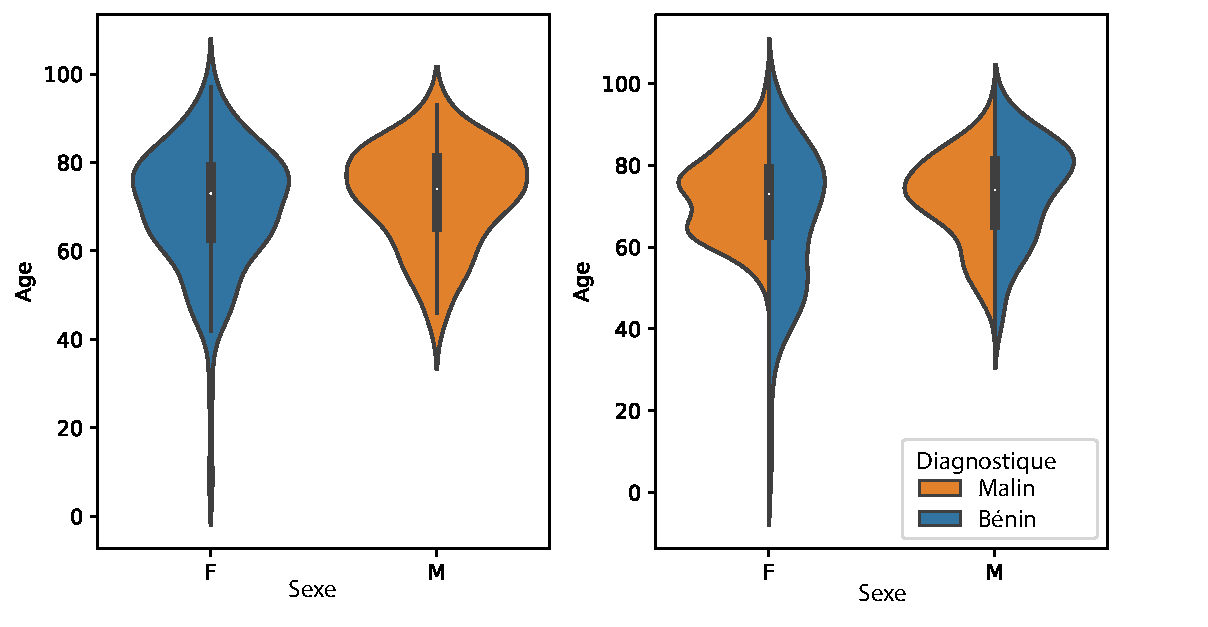
\includegraphics[width=0.8\linewidth]{contents/chapter_2/resources/statistics.pdf}
    \caption{A gauche, répartition en fonction de l'âge et du sexe. A droite, répartition entre l'âge et le sexe en tenant compte du diagnostique binaire.}
    \label{fig:statistics}
\end{figure}\par

En ce qui concerne leur acquisition, celle-ci a à chaque fois été réalisée par l'un des 3 experts investigateurs de l'étude clinique~\cite{Cinotti2018}. Tout cas de collisions de tumeurs au sein d'un même groupe a été exclue de cette étude. En ce qui concerne la modalité de dermatoscopie, les données ont été produites à l'aide d'une caméra PowerShot® G7~\textsuperscript{\ref{footnote:device_powershot}} couplé au dispositif proposé par Fotofinder~\textsuperscript{\ref{footnote:device_fotofinder}}. Pour ce qui est de la modalité de \gls{rcm}, les données proviennent d'une caméra VivaScope 3000®~\textsuperscript{\ref{footnote:device_mavig}}. En revanche, aucune information lié à l'acquisition des données de photographie clinique n'a été mentionnée.\par

L'intérêt de ces trois modalités est grand dans le contexte dermatologique puisqu'elles représentent le processus "classique" de prise en charge clinique, de la modalité la moins onéreuse avec la \textbf{photographie clinique} mais également la moins précise, à la modalité la plus onéreuse et apportant un degrés d'information plus important avec la \textbf{\gls{rcm}}. Ainsi, chaque modalité permet de réduire ainsi la zone d'incertitude chez un patient souffrant d'une pathologie de lapeau.

\addtocounter{footnote}{1}
\footnotetext[\thefootnote]{Source : Canon Powershot®, Canon, Tokyo, Japon. \label{footnote:device_powershot}}
\addtocounter{footnote}{1}
\footnotetext[\thefootnote]{Source : FotoFinder Systems GmbH, Bad Birnbach, Allemagne. \label{footnote:device_fotofinder}}
\addtocounter{footnote}{1}
\footnotetext[\thefootnote]{Source : Distribué en Europe par MAVIG GmbH, Munich, Allemagne. \label{footnote:device_mavig}}

\subsection{Protocole d'évaluation des experts}
Afin d'évaluer les performances de praticiens face à ces lésions, les investigateurs ont eu recours à 21 dermatologues détenant une expertise des modalités d'imagerie non invasives. Ces experts sont réparti de manière homogène selon leur compétences respectives pour chacun des dispositifs. Ainsi, le panel d'évaluation se décompose de la façon suivante: 
\begin{inlinerate}
\item 6 experts sont soumis à l'ensemble des modalités,
\item 15 experts sont soumis à l'évaluation de la photographie clinique et de la dermatoscopie (dont 6 sur l'ensemble et 9 uniques)
\item et 12 sont soumis à la \gls{rcm} (dont 6 sur l'ensemble et 6 uniques)~\cite{Cinotti2018}.
\end{inlinerate}
Cette répartition est résumée en \Cref{fig:experts_evaluation}. Pour chaque cas clinique étudié, ces experts ont évalué la gravité du cas à l'aide des termes bénin et malin.\par

\begin{figure}[H]
    \centering
    \includegraphics[width=0.6\linewidth]{contents/chapter_2/resources/experts_evaluation.pdf}
    \caption{Répartition du panel de 21 dermatologues sur l'évaluation des diverses modalités~\cite{Cinotti2018}.}
    \label{fig:experts_evaluation}
\end{figure}\par

Pour éviter tout biais dans l'évaluation, les experts évalués sur l'ensemble des modalités ont contactés sur 3 journées différentes: 
\begin{inlinerate}
\item une première évaluation sur images de photographie clinique et dermatoscopie,
\item une seconde évaluation sur images de \gls{rcm}
\item et une dernière évaluation sur l'ensemble des images.
\end{inlinerate}
Par ailleurs, les images ont été présentée dans un ordre différents enter chaque journée d'évaluation. De plus, l'évaluation sur base d'image de photographie clinique a toujours été réalisée avant la dermatoscopie.\par

\subsection{Résultats des experts}

\subsection{Structuration de la base}
Afin de réaliser nos divers tests, une base d'images anonymisée nous a été remise, composée :
\begin{itemize}
\item d'un fichier tableau de lésions comprenant:
    \begin{inlinerate}
        \item en colonne, les diverses informations: \textit{Âge, Sexe,	Zone, Côté,	Diagnostic Binaire et Diagnostic},
        \item en ligne, les divers enregistrement liée à chaque lésion.
    \end{inlinerate}
    \item d'un répertoire comprenant les images des divers cas clinique recensé dans l'étude sous divers format image.
\end{itemize}\par

Afin d'exploiter au mieux cette base, quelques modifications y sont apportées. D'une part, la diversité des formats images est un frein quand à la gestion de ces données et nous avons opté pour un format matriciel sans perte de type bitmap. D'autre part, la structure de la base ne permet pas l'utilisation d'annotation au niveau des images ou des instances autres. Afin de rendre plus dynamique cette partie, nous avons opté pour une structure reprenant le fichier table initial (au format \gls{csv}) et de répertoires associés à chaque lésion. Chaque dossier de lésion se compose lui même de fichiers d'annotation propre au type de données stockées (images ou patchs). Par ailleurs, certaines ajout d'informations tel que l'appartenance à un patient ont été ajouté pour la suite de notre travail. La \Cref{fig:db_structure} synthétise la structure de cette base avant et après modification.\par

\begin{figure}[H]
\centering
    \begin{subfigure}{.45\textwidth}
      \centering
      \includegraphics[width=\linewidth]{contents/chapter_2/resources/db_structure_old.pdf}
    \end{subfigure}
    \begin{subfigure}{.45\textwidth}
      \centering
      \includegraphics[width=\linewidth]{contents/chapter_2/resources/db_structure_new.pdf}
    \end{subfigure}
    \caption{Schématisation de la base de ressources employé. A gauche, la base initiale et à droite, la base restructurée afin de supporter de nouvelles annotations.}
    \label{fig:db_structure}
\end{figure}\par

\renewcommand{\thechapter}{\arabic{chapter}}
\setcounter{chapter}{2}

\chapter{Intelligence artificielle et notions complémentaires}
\label{chap:chapter_3}
\chapterintro
Lors du précédent chapitre, les interactions entre la peau et la lumière ont été abordées, ainsi que les dispositifs majeurs permettant l'acquisition d'informations de la peau.\par

Actuellement, l’informatique est une ressource omniprésente dans de nombreux domaines d’application. Ses facultés à divertir ou encore à guider ses usagers dans leurs choix quotidiens personnels et professionnels en font un précieux allié. De nouvelles pratiques font leurs apparitions, intégrant la machine au cœur des processus décisionnels. Les disciplines médicales évoluent largement et l’ordinateur permet de répondre aux besoins croissants de précision, de reproductibilité intra et inter opérateur, et permet un gain de temps au sein des milieux cliniques. Dans un cadre bien défini, il s’agit également d’un moyen de formaliser la connaissance au travers d’un outil pouvant être utilisé par des non-initiés.\par

Cette nouvelle partie permet de dérouler un peu plus le plan de ce manuscrit, en abordant cette fois-ci les systèmes d'intelligence artificielle et leur utilité vis à vis des données médicales de ce manuscrit.\par
\newpage

\section{Généralités sur l'intelligence artificielle}
\label{sec:artificial_intelligence}
La notion \textbf{d’\gls{ia}} est assez souvent contestée, mais se définit plus généralement comme étant «~l’ensemble de théories et de techniques mises en œuvre en vue de réaliser des machines capables de simuler l'intelligence humaine~»~\textsuperscript{\ref{footnote:ia_larousse}}. Ainsi, dans cette définition, ces techniques ne se limitent pas à la reproduction du comportement interactif social humain souvent représenté dans les médias. La mise en pratique sous forme informatique de mécanismes dédiés à la prise de décision à partir de données ou encore, la retranscription du raisonnement d'un expert fait partie de cette définition.\par

Une vision plus complète de ce terme consiste à décomposer l'\gls{ia} en une discipline organisée en sous domaines possédant chacun leurs spécificités, comme schématisé sur la \Cref{fig:scheme_overview_ia}. Ainsi, le terme \textbf{d'apprentissage automatique} ou de \textit{machine learning} caractérise un premier sous champ de l'\gls{ia} et est employé pour qualifier l'utilisation de mécanismes statistiques dans le but de générer des règles, à partir de données d'apprentissage. Ces données étant souvent complexes, il est souvent nécessaire de laisser l'humain intervenir pour extraire l'information pertinente à l'accomplissement de la tâche souhaitée. Enfin, le terme \textbf{d'apprentissage profond} ou de \textit{Deep Learning} désigne un sous champ de l'apprentissage automatique, dans lequel des couches succesives de prises de décision vont permettre d'augmenter la complexité des relations entre les données d'entrée et les tâches.\par

\addtocounter{footnote}{1}
\footnotetext[\thefootnote]{Source~: Encyclopédie Larousse. \label{footnote:ia_larousse}}

\begin{figure}[H]
    \centering
    \includegraphics[width=\linewidth]{contents/chapter_3/resources/scheme_overview_ia.pdf}
    \caption{Représentation des relations entre \textit{intelligence artificielle}, \textit{apprentissage automatique} et \textit{apprentissage profond}.}
    \label{fig:scheme_overview_ia}
\end{figure}\par

Cette partie a pour vocation d’amener à la compréhension générale des courants d’\gls{ia}, qui permettent la résolution de problématiques variées telles que la dermatologie. Dans une première section, les approches par apprentissage sont décrites, puis par extension amène à la présentation de l'apprentissage profond dans une seconde section. La troisième section décrit les méthodes permettant le paramétrage et l'évaluation de ces modèles. Enfin, la dernière section décrit les principes de fusions utiles à ce travail.\par

\section{Approches par apprentissage}
\label{sec:machine_learning}
Ce courant a été \textit{évoqué} en 1948 par Alan Turing ; son idée était de proposer des «~machines à apprendre susceptibles de construire elles-mêmes leurs propres codes~»~\cite{Turing1950}. En 1959, Arthur Samuel formule une première définition des approches par apprentissage comme étant un « domaine d’étude dans lequel la possibilité est donnée à l’ordinateur d’apprendre sans avoir été explicitement programmé ».\par 

Les approches par apprentissage automatique peuvent être résumées aux techniques permettant à un système informatique d’adapter son analyse et son comportement en fonction de ses données d’entrée. Une définition plus formelle et récente de ce domaine proposée par Tom Michael Mitchell est qu’un «~programme informatique apprend d’une expérience $E$, en adéquation avec des tâches $T$ et une mesure de performance $P$, si sa performance sur les tâches $T$, mesurée par $P$, s’améliore avec l’expérience $E$~».\par

Ainsi au sein des courants d’apprentissage, deux grandes sous catégories synthétisées dans la \Cref{fig:scheme_machine_learning} peuvent être distinguées, dont~: 
\begin{itemize}
    \item l'apprentissage \textbf{supervisé} correspond aux techniques visant à faire correspondre les données d'entrée avec des sorties de valeurs discrètes (on parle aussi de classification) ou continues (on parle alors de régression),
    \item l'apprentissage \textbf{non-supervisé} correspond à des approches exploratoires, dans lesquelles l'ordinateur tente d'identifier des corrélations au sein des données (désigné par le terme de \textit{clustering}),
    \item l'apprentissage \textbf{semi-supervisé}~\cite{Murphy2012} reprend les précédentes théories afin d'exploiter au mieux l'ensemble des données à disposition et de mieux discerner le problème.
\end{itemize}

Les prochaines sous-sections de ce chapitre abordent chacune de ces catégories respectives de manière plus détaillée.\par
 
\begin{figure}[H]
    \centering 
    \includegraphics[width=\linewidth]{contents/chapter_3/resources/scheme_machine_learning.pdf}
    \caption{Schéma de décomposition des approches par apprentissage automatique.}
    \label{fig:scheme_machine_learning}
\end{figure}

\subsection{Apprentissage supervisé}
\label{sec:supervised_learning}
L’apprentissage supervisé consiste à déterminer la relation permettant de faire correspondre des données d’entrée $x$ et des données de sorties $y$ et cela, dans le but de produire sur de nouvelles données d’entrée $x'$, de nouvelles sorties $y'$.\par

Cette approche implique l’utilisation d’une base d’apprentissage, définie comme \textit{un ensemble de couples entrée-sortie} noté $\{(x_1,y_1 ),\ldots,(x_n,y_n )\}$ avec $n \in N$. Ainsi, l’humain tente d'apporter une signification à ces données sous forme d'annotations (ou étiquettes) pour lesquelles la machine devra être en mesure de déterminer la relation existante.\par

Dans le but d'achever cette tâche, les variables propres à chaque observation sont supposées suffisamment discriminantes pour permettre l'identification des annotations. Ce problème est défini par la relation $y=f(x)$, où $f$ est une fonction inconnue correspondant au phénomène observé, par une fonction d’approche $g$ appelée fonction de prédiction tel que $y=g(x)$, avec $x=\{x_1,x_2,\ldots,x_n\}$ un vecteur de caractéristiques possédant suffisamment d'information~\cite{foulds2010}.\par 

Cet apprentissage, schématisé sur la \Cref{fig:scheme_supervised_classification}, se découpe en deux processus distincts~:
\begin{itemize}
    \item \textbf{l’apprentissage} ou \textit{entraînement}, qui consiste à approcher la fonction $f$ par une fonction $g$ compte tenue de données étiquetées,
    \item \textbf{la prédiction} ou \textit{inférence}, qui consiste à prédire sur de nouvelles données à partir de $g$ tel que $g(x') = y'$.
\end{itemize}\par

\begin{figure}[H]
    \centering
    \includegraphics[width=\linewidth]{contents/chapter_3/resources/scheme_supervised_classification.pdf}
    \caption{Schéma de l’approche dite supervisée. La phase d'entraînement permet de déterminer les relations entre données et attentes, sur des données connues dites d'apprentissage. La phase de prédiction réutilise les relation déterminées lors de la phase d'entraînement. }
    \label{fig:scheme_supervised_classification}
\end{figure}
\clearpage

Ces approches dites supervisées se regroupent ainsi au travers de deux catégories majeures~:
\begin{itemize}
    \item la \textbf{classification}, c’est-à-dire la prédiction de valeurs discrètes, soit l’ensemble des entiers relatifs noté $\pmb{\mathbb{Z}}$. Sont également utilisés les compléments de \textit{classification binaire} lorsque le problème formulé ne comporte que deux classes, et de \textit{classification multi-classes} lorsque la situation nécessite de prédire $N$ classes avec $N > 2$.
    \item la \textbf{régression}, c’est-à-dire la prédiction de valeurs continues, soit l’ensemble des nombres réels noté $\pmb{\mathbb{R}}$.
\end{itemize}\par

Les travaux de ce manuscrit portent sur les méthodes de classification, qui se traduisent par la catégorisation d'images cliniques pathologiques ou de lésions selon divers niveau de dangerosité. En prenant appui sur l'un des travaux~\cite{Kotsiantis2007}, une synthèse de ces méthodes et de leur principe respectif est fourni, dont~:
\begin{itemize}
    \item \textbf{les approches logiques} qui correspondent à des approches par succession de décisions~\cite{Kotsiantis2007}. Dans cette catégorie, le principal représentant est celui des arbres de décision~\cite{Breiman1984}, également connu sous le terme de \gls{cart}, dont le principe peut se résumer à la construction d'un graphe, dans lequel chaque noeud est associé à une décision définie par le choix d'une caractéristique et d'un seuil~\cite{Quinlan1986}. Toute la complexité de ces approches repose sur le choix de ces caractéristiques dont la priorité dépend de l'ordre d'importance dans la séparation du problème.
    \item \textbf{les approches statistiques} qui correspondent à des approches probabilistes, qui déterminent la probabilité d'appartenance d'un élément à une classe. Le \gls{nbm}~\cite{Zhang2004} est un exemple typique de ce type d'approche, dans lequel chaque caractéristique est considérée comme indépendante. La relation entre caractéristique et annotation se définit ainsi comme le produit des probabilités de chacune d'entre elles d'appartenir à la classe supposée (voir l'\Cref{eq:bayesian}). Ce type de classification bayésienne peut également être étendue sous la forme de réseau~\cite{Kononenko1989}.
    \item \textbf{les approches par instances} qui qualifient des méthodes consistant à une accumulation des échantillons afin d'enrichir un espace et non pas de leur interprétation menant à une forme de connaissances. La méthode la plus connue reposant sur ce principe est celle des \gls{knn}~\cite{Cover1967}, dont la théorie majeure repose sur l'appartenance d'une donnée à une classe si celle-ci est suffisamment proche par ses caractéristiques, d'échantillons pré-existants de cette dernière. Il est alors nécessaire de définir un critère de distance, le principal utilisé étant celui de la distance euclidienne. 
    \item \textbf{les approches par \gls{svm}}~\cite{Cortes1995} correspondent à des approches assez récentes dont le principe se résume à déterminer une frontière de séparation entre les diverses classes, qui maximise une marge suffisante permettant entre autres une meilleure tolérance au bruit. Afin de déterminer au mieux cette frontière, divers noyaux ont été établis dont le plus simple d'entre eux est \textbf{le noyau linéaire}. La présence \textbf{d'un noyau de fonction de base radiale} ou \textit{Radial Basis Function} est à préciser, considéré comme un \textit{approximateur universel} si les données à disposition sont suffisantes~\cite{Wang2004}.
    \item \textbf{les approches par ensembles} sont une catégorie qui qualifie les méthodes qui emploient un ensemble de modèles prédictifs afin de construire un unique modèle plus robuste. L'une de ces méthodes, les \gls{rf}~\cite{Breiman2001} sont une extension du principe d'arbre de décision précédemment évoqué, destiné à réduire le risque de sur-apprentissage du modèle initial. Cette méthode réalise $N$ sélections aléatoires d'observations, pour lequel $N$ arbres de décision sont générés. Afin de diversifier ces arbres, un mécanisme de tirages aléatoires de caractéristiques est également réalisé au niveau de chaque noeud de décision. Une autre de ces méthodes, l'\gls{gb} est un mode opératoire généralement constitué par des arbres de décisions. En opposition avec les \gls{rf} où chaque arbre de décision correspond à un modèle de prédiction faible, l'\gls{gb} consiste à diminuer de manière séquentielle une fonction de coût à chaque nouvel arbre généré~\cite{Friedman2001}.
\end{itemize}\par

\begin{equation} 
    \label{eq:bayesian}
    \hat{y} = \underset{k \in \{1, \ldots, K\}}{\operatorname{argmax}} \ p(C_k) \displaystyle\prod_{i=1}^n p(x_i \mid C_k)
\end{equation}

Devant ces nombreuses méthodes, il est difficile de déterminer un modèle optimal à une situation particulière, notamment dans le cadre de données à forte complexité. En effet, une évaluation de manière empirique de ces diverses méthodes reste encore la meilleure solution afin de déterminer ce modèle optimal, en contrepartie d'un temps de calcul important. Néanmoins, l'un des travaux menés sur la performance des modèles supervisés, a permis de déterminer un certain nombre de critères de comparaison entre ces diverses techniques mettant en valeur en général les avantages et inconvénients de chacune d'entre elles~\cite{Kotsiantis2007}.\par

Pour cela, la \Cref{tab:model_comparison} recense la plupart des critères importants évoqués par ce travail de recherche. La performance de classification notamment, qui semble indéniable dans le champ que ce travail tente d'évaluer avec une emphase forte en termes de performances pour les \gls{svm}. La vitesse d'apprentissage a également été précisée à titre indicatif. En effet, bien que contraignante lors des expérimentations de ce manuscrit, elle ne constitue pas un frein et reste le principal inconvénient des \gls{svm}. Enfin, ces derniers sont reconnus comme robustes face à des situations pouvant comporter des caractéristiques non pertinentes ou redondantes.\par

À la vue de ces éléments, il semble plus que nécessaire de considérer l'utilisation des \gls{svm} au sein de ces travaux. De même, il est nécessaire de considérer l'utilisation des deux méthodes d'approches par ensemble mentionnées, les \gls{rf} et l'\gls{gb}, pour lesquelles aucun travail comparatif généraliste n'a été trouvé. Néanmoins, une étude génomique semble plaider dans le sens des \gls{svm} et de l'\gls{gb}~\cite{Ogutu2011}. Pour finir, il est également nécessaire de considérer ces modèles de classification au sein de processus proposés par des travaux proches de cette thématique. Ces éléments sont abordés plus en détail dans leur partie respective.\par

\begin{table}[H]
  \small
  \centering 
    \begin{tabular}{lcccc}
        \toprule
                                                                    & \textbf{\gls{cart}}   & \textbf{\gls{nbm}}& \textbf{\gls{knn}}    & \textbf{\gls{svm}}\\
        \midrule
        \textbf{Performances de classification}                     & **                    & *                 & **                    & ****              \\
        \midrule
        \textbf{Vitesse d'apprentissage}                            & ***                   & ****              & ****                  & *                 \\
        \midrule
        \textbf{Tolérance aux caractéristiques non pertinentes}     & ***                   & **                & **                    & ****              \\
        \midrule
        \textbf{Tolérance aux caractéristiques redondantes}         & **                    & **                & **                    & ***               \\
        \bottomrule
  \end{tabular}
  \caption{Table de comparaison des méthodes d'apprentissage majeures de la littérature~\cite{Kotsiantis2007}. Ce tableau propose un système de notations allant de une (mauvaise performance) à quatre étoiles (bonne performance).}
  \label{tab:model_comparison}
\end{table}
\clearpage

\subsection{Apprentissage non-supervisé}
\label{sec:unsupervised_learning}
L’apprentissage non supervisé ou \textit{descriptif} est une seconde approche d’apprentissage dans laquelle l’ordinateur tente de \textit{découvrir} en autonomie, des corrélations au sein de jeux de données. Ces approches émergent de problématiques diverses, telles que~:
\begin{itemize}
    \item la \textbf{réduction des coûts} le plus souvent humain nécessaire à l’obtention de données annotées, c’est-à-dire de données pour lesquelles les couples d’entrées et de sorties sont connus.
    \item la \textbf{découverte des diverses relations} pouvant exister au sein d’un amas de données. En effet, une annotation ne correspond qu'à un échantillon de l’information et ne permet pas d’obtenir les relations pouvant régir des modèles d'interactions complexes.
    \item l'\textbf{exploration de nouvelles relations} de type \textit{cause – effet}, en réaction à la masse de données produites par les objets connectés.
\end{itemize}\par

Ce principe est concrétisé aux travers de méthodes, comme les k-moyennes qui tentent de déterminer des correspondances en minimisant la différence d’énergie entre les points d’un même groupe, dont un schéma est visible sur la \Cref{fig:scheme_unsupervised}. Diverses applications peuvent ainsi en résulter, telles que~:
\begin{itemize}
	\item le \textbf{regroupement par classes de données}, afin de définir de manière automatique de nouvelles annotations.
	\item la \textbf{réduction de dimensions}, dans le but de ne conserver que l'information essentielle. La méthode du \textit{bag-of-words} est un exemple initialement prévue pour l'analyse de texte~\cite{Zhang2010} et utilisée dans des domaines tels que l'analyse d'image de la peau~\cite{Situ2008}.
	\item la \textbf{découverte de relations} au sein de l’information, et des relations les plus robustes entre variables et dépendances.
\end{itemize}\par

\begin{figure}[H]
    \centering
    \includegraphics[width=0.9\linewidth]{contents/chapter_3/resources/scheme_unsupervised.pdf}
    \caption{Exemple de données non associées à des annotations préalables, et pour lesquelles des approches non supervisées peuvent être sollicitées afin de découvrir des groupes de données ou \textit{clusters}. Le nombre de groupes le plus souvent défini par l’utilisateur avant traitement, influe fortement la vision du problème.}
    \label{fig:scheme_unsupervised}
\end{figure}

\subsection{Apprentissage semi-supervisé}
\label{sec:semisupervised_learning}
Les techniques d'apprentissage semi-supervisé tentent de combiner les deux principes précédents et sont la conséquence du coût de l'annotation des données qui nécessite souvent le travail d'experts. En effet, il peut être difficile d'avoir accès à une vérité terrain qui couvre la totalité d'un jeu de données sans pour autant perdre l'apport de cette information non-annotée. Ce dernier point est particulièrement intéressant dans le cadre de données à grande dimensions pour lesquelles \textbf{l'espace} des dimensions croît de manière exponentielle et \textit{dilue} les échantillons (connu sous le terme de \textit{fléau des dimensions}~\cite{Donoho2000}).\par 

Ainsi, l'apprentissage semi-supervisé se base sur plusieurs hypothèses auxquelles doivent se confronter les données~\cite{Zhu2009}, dont~:
\begin{itemize}
	\item un critère \textbf{d'homogénéité}, c’est-à-dire que des données issues d'une zone de haute densité partagent les mêmes annotations, 
	\item un critère \textbf{de séparation par faible densité}, c’est-à-dire que s'il existe une  séparation entre plusieurs types d'annotations, celle-ci se situant dans une zone à faible densité~\cite{chapelle2005}.
\end{itemize}
En pratique, il est difficile de s'assurer que des données mises à disposition respectent bien ces engagements. Afin de mieux visualiser ce concept, l'exemple en \Cref{fig:example_semi_supervised} démontre l'intérêt de telles approches. Ce principe permet d'éviter d'extrapoler des frontières difficilement définissables dans une situation de faible densité de l'information étiquetée.\par
 
\begin{figure}[H]
    \centering
    \includegraphics[width=\linewidth]{contents/chapter_3/resources/example_semi_supervised.pdf}
    \caption{Exemple fréquemment employé pour démontrer l'intérêt de l'apprentissage semi-supervisé du point de vue du principe de densité. À gauche, une classification obtenue à partir de deux données étiquetées ; À droite, la même situation avec l’ajout de données non étiquetées.}
    \label{fig:example_semi_supervised}
\end{figure}

\clearpage

\section{Apprentissage profond}
\label{sec:deep_learning}
L’apprentissage profond correspond à un sous-ensemble de l’apprentissage automatique, encouragé par les récents apports des neurosciences sur le fonctionnement et le rôle des neurones sur la prise de décisions complexes~\cite{Quartz1997,Shrager1996}. En effet, le cerveau possède divers niveaux de traitement de l’information, ce que tente d'imiter l'apprentissage profond par l'apport de multiples couches de traitement.\par

En effet, dans le cadre des méthodes \textit{classiques} d’apprentissage évoquées dans la partie précédente, la dimension de \textit{couches} de traitement n’est pas intégrée. Les approches par apprentissage simple proposent une architecture en trois couches, dont l’une des couches est allouée à la corrélation entre les données d’entrée et de sortie. Par opposition, les approches par apprentissage profond proposant des structures en $n$ couches, avec $n \in \pmb{\mathbb{N}}$ et $n>1$. Ces couches intermédiaires sont également qualifiées de couches cachées.\par 

Dans une première sous-section, une brève présentation du principe de \gls{ann} est réalisé, puis dans une seconde sous-section est détaillée leur extension au \gls{cnn}. Enfin, les aspects liés au principe de transfert de connaissances sont proposés dans une dernière sous-section.\par

\subsection{Réseau de neurones artificiels}
Les \gls{ann} sont des structures multicouches composées d'unités basiques appelées neurones. Dans ce schéma, chaque neurone ou unité est connecté à l'ensemble des unités de la couche $N-1$ et $N+1$ et forme un \textit{maillage}.\par

Les neurones se partagent ainsi l'information de point à point de l'entrée vers la sortie, appliquant respectivement l'opération dont ils sont responsables. Cette opération au sein d'une unité est de la forme $y = W\mathbf{x}+\mathbf{b}$ dans laquelle $W$ représente une matrice de poids qui permettra de pondérer les signaux des prédécesseurs et $b$ un terme de correction appelé biais~\cite{Stephen1990}. Ainsi, les neurones en entrée d'un réseau reçoivent une information \textit{brute} tandis que, les neurones situés en sortie du réseau reçoivent une information pré-traitée par les prédécesseurs. Le schéma présent sur la \Cref{fig:scheme_deep_understanding} permet de mettre en évidence un cas simple de résolution par apprentissage pour appréhender cette notion.\par

Néanmoins, cet exemple met également en avant que ce même modèle pourrait être représenté à l'aide d'une fonction d'ordre suffisante~\cite{Bishop2006}. Ce mécanisme seul ne suffit pas à créer des réseaux exploitant les bénéfices d'un tel agencement. En effet, si une unité de ce réseau est représentée par $y = W\mathbf{x}+\mathbf{b}$, une succession de ces unités pourrait se résumer à la fonction linéaire représentée par l'\Cref{eq:proof_linearity}~\textsuperscript{\ref{footnote:equation_andrewng}}. Afin de tirer parti du potentiel de ce choix d'agencement en couches, ont été introduites des fonctions d'activation (tanh, ReLu, \ldots) qui permettent d'introduire une non-linéarité au sein de ces réseaux, permettant notamment l’autodétermination de structures de décision complexes.\par

\begin{equation} 
    \label{eq:proof_linearity}
    \begin{split}
        y = h(\mathbf{x})   &=\mathbf{b}_n+W_n(\mathbf{b}_{n-1}+W_{n-1}(\dots (\mathbf{b}_1+W_1 \mathbf{x})\dots))\\
                            &=\mathbf{b}_n+W_n\mathbf{b}_{n-1}+W_nW_{n-1}\mathbf{b}_{n-2}+\dots+W_nW_{n-1}\dots W_1\mathbf{x}\\
                            &=\mathbf{b}'+W'\mathbf{x}
    \end{split}
\end{equation}\par

\addtocounter{footnote}{1}
\footnotetext[\thefootnote]{Source~: Plateforme de cours en ligne \href{https://www.deeplearning.ai/}{Deep Learning AI}, démonstration par Andrew Ng. \label{footnote:equation_andrewng}}

Un très bon représentant de ces types de réseaux est le \gls{mlp} utilisé à des fins de classification. Par ailleurs, un inconvénient majeur de ces réseaux est le grand nombre d'hyperparamètres à disposition. Il est ainsi délicat de procéder au choix du nombre de neurones ou même de celui des fonctions d'activation.\par

\begin{figure}[H]
    \centering
    \includegraphics[width=\linewidth]{contents/chapter_3/resources/scheme_deep_understanding.pdf}
    \caption{Exemple simplifié d'une structure d’apprentissage profond. Ce modèle se compose de deux couches intermédiaires cachées~: la première couche extrait des caractéristiques linéaires simples, tandis que la seconde couche par combinaison avec la première couche conduit à une extraction de caractéristiques plus complexes. Ainsi, la première couche s'apparente à un polynôme de degré 1, tandis que la seconde couche représente des fonctions de degré 2 et ainsi de suite.}
    \label{fig:scheme_deep_understanding}
\end{figure}

\subsection{Réseau neuronal convolutif}
\label{sec:convolutionnal_neural_network}
Les \gls{cnn} sont une extension des réseaux de neurones profond, essentiellement utilisés dans un but de traitement de l'image. Moins développé par la littérature, ce principe de réseaux peut être étendu à des données telles que des signaux (1D) ou des volumes (3D).\par

Ces \gls{cnn} sont une réponse à l'application des \gls{ann} à des problématiques impliquant des données images et des contraintes multiples qu'ils comportent. Parmi ces contraintes de l'application des \gls{ann} aux images, peuvent être évoqués~: 
\begin{inlinerate}
    \item les \textbf{nombreuses connexions et paramètres requis},
    \item l'\textbf{absence d'utilisation de la cohérence de l'information spatiale},
    \item et la \textbf{dépendance} du réseau à la taille des informations d'entrée.
\end{inlinerate}\par

Ainsi, ces réseaux font appel à des couches de convolution permettant de résoudre ces trois principales contraintes. D'une part, la convolution permet de réduire fortement le nombre de paramètres d'entraînement, le réseau n'est ainsi plus entièrement \textit{connecté}. Certaines optimisations récentes consistent à remplacer les filtres de convolution 2D par une succession de filtres 1D horizontaux et verticaux, proposant des résultats semblables et réduisant fortement le nombre de paramètres. D'autres part, la convolution permet d'apporter une logique à la dimension spatiale des données ainsi qu'une indépendance à la taille. En effet, le réseau n'est plus entièrement connecté et donc ne dépend plus d'une taille fixe, et peut ainsi traiter des données de tailles différentes mais qui doivent respecter une taille minimum. Le traitement des données par ces couches de convolution porte le nom de carte d'activation, maximum quand le produit de convolution est en phase.\par

% \begin{equation} 
%     \label{eq:convolution_integral}
%     \begin{split}
%         (f\ast g) (x) = \int_{-\infty}^{+\infty} f(x-t)g(t) \, \mathrm dt = \int_{-\infty}^{+\infty} f(t)g(x-t) \, \mathrm dt
%     \end{split}
% \end{equation}

\clearpage

\subsection{Transfert de connaissances}
\label{sec:transfer_learning}
L’apprentissage par transfert est une technique connexe à l’apprentissage profond défini comme « faisant référence à la situation où ce qui a été appris dans un contexte \ldots est exploité pour améliorer la généralisation dans une autre contexte »~\cite{Ngiam2011}. Cette discipline s’inscrit dans le champ de \textbf{l’adaptation de domaine}, définie comme le transfert des connaissances d’un domaine $D_S$, défini par l’hypothèse $h: X_S \rightarrow Y_S$, vers un domaine cible $D_T$ afin de satisfaire $h: X_T \rightarrow Y_T$. Son champ d'application n'est pas limité aux réseaux d'apprentissage profond, mais les contraintes qui leurs sont associées font de ces techniques une ressource utile.\par

En effet, ces solutions permettent de réduire les difficultés liées à la grande quantité de ressources de calcul, de temps, mais également de données mobilisées nécessaires à un entraînement depuis sa base. Le modèle d’apprentissage attendu est alors initialement plus performant, croît plus efficacement et est plus performant qu’un apprentissage spécifique (\Cref{fig:learning_curves}).\par

Néanmoins, cette solution n’est envisageable que lorsque l’apprentissage, réalisé lors de la première tâche, généralise suffisamment le phénomène observé. Ainsi, il est d’usage courant de ne spécifier lors du transfert que la couche finale de classification du réseau, les premières couches étant employées comme extracteur général de caractéristiques. Toutefois, certaines méthodes de la littérature s’accordent sur l'entraînement conjoint des couches de classification ainsi que des couches de convolutions hautes, considérées comme moins génériques.\par

\begin{figure}[H]
    \centering
    \includegraphics[width=\linewidth]{contents/chapter_3/resources/example_learning_curves.pdf}
    \caption{Exemple d'attentes liées à un apprentissage par transfert en opposition à un apprentissage classique.}
    \label{fig:learning_curves}
\end{figure}
\clearpage

\section{Paramétrage et évaluation de modèles prédictifs}
\label{sec:models_settings}
Cette partie se concentre sur l'évaluation de modèles de prédiction et présente la problématique de \textbf{biais}. Ses origines et ses risques associés sont présentés ainsi que les potentielles méthodes permettant de s'en affranchir.\par

\subsection{Généralisation de modèles}
\label{subsec:generalized_models}
À l'aide de couples d'entrée et de sortie mis à disposition, ces modèles sont capables d’apprendre une relation en la \textit{généralisant} et d’estimer de nouvelles sorties sur de nouvelles données. Il est pour cela nécessaire de parvenir à isoler l'information responsable de ce cheminement, plus ou moins séparable, en cause souvent la qualité de~:
\begin{inlinerate}
    \item l'hypothèse formulée, c’est-à-dire si la relation qui lie l'observation et sa conséquence est directe mais également vraie dans toute circonstance,
    \item l'information possédée, c’est-à-dire si l'information est juste pour répondre à la problématique cible (qualité de l'observation, rapport signal sur bruit, \ldots).
\end{inlinerate}\par 

Ce problème, évoqué dans la littérature porte le nom de « dilemme de biais et variance », dans lequel le biais représente le manque de relation pertinente entre données d’entrée et de sortie et où la variance représente l’influence du modèle au petites fluctuations souvent issues de bruit. Ces termes sont intrinsèquement liés aux problématiques respectives de \textbf{sous-apprentissage} et \textbf{sur-apprentissage}. La \Cref{fig:example_underfit_overfit} reprend de manière visuelle ces problématiques, et les exprime selon un jeu d’entraînement et de test. À noter que le sur-apprentissage peut être limité par l’utilisation de termes de régularisation, de schémas de validation de modèle adaptés ou l’utilisation d’ensembles de données suffisantes.\par
 
\begin{figure}[H]
    \centering
    \includegraphics[width=0.85\linewidth]{contents/chapter_3/resources/example_underfit_overfit.pdf}
    \caption{Exemple de dilemme de biais et de variance. À gauche, un cas de sous-apprentissage, ce modèle est une sous approximation du phénomène observé. À droite, un cas de sur-apprentissage, le modèle ne généralise pas suffisamment le phénomène observé.}
    \label{fig:example_underfit_overfit}
\end{figure}

\subsection{Choix de métriques}
\label{subsec:metrics}
Le choix des métriques représente une part importante de la problématique de ce manuscrit pour la mise en place de modèles d’apprentissage. D'une part, ce choix permet d'orienter la sélection d'un modèle en particulier et d'autre part, permet de retenir les performances attendues par ce dernier sur des données extérieures au jeu de données employé.\par

L’un des principaux outils à disposition afin d'évaluer la performance est la matrice de confusion, schématisé sur la \Cref{fig:scheme_confusion_matrix}. Elle permet de faire correspondre les classes réelles et prédites~: la diagonale de cette matrice fait figurer les prédictions correctement réalisées par le modèle, tandis que les éléments restants renseignent sur les prédictions erronées. Dans une situation à deux classes ou \textit{binaire}, cette matrice fait ainsi ressortir quatre mesures~:
\begin{itemize}
	\item les \textbf{vrais positifs}, les éléments de la classe positive détectés comme positif,
	\item les \textbf{vrais négatifs}, les éléments de la classe négative détectés comme négatif,
	\item les \textbf{faux positifs}, les éléments de la classe négative détectés comme positifs,
	\item les \textbf{faux négatifs}, les éléments de la classe positive détectés comme négatifs.
\end{itemize}\par

\begin{figure}[H]
    \centering
    \includegraphics[width=\linewidth]{contents/chapter_3/resources/scheme_confusion_matrix.pdf}
    \caption{Schéma représentatif d’une matrice de confusion, qui met en avant une situation binaire.}
    \label{fig:scheme_confusion_matrix}
\end{figure}

Bien que déjà réduite, l'information de cette matrice est encore très riche et difficile à utiliser comme critère de sélection. Pour cela, diverses métriques éprouvées sont à envisager selon la problématique de recherche. Parmi les plus courantes d'entre elles, les critères de \textbf{précision}, \textbf{sensibilité} (également appelé \textbf{rappel}) ou encore \textbf{spécificité} sont pléthores dans la littérature mais ont tendance à ne capter qu'une partie du problème. Par exemple, la sensibilité est un critère très important en médecine ou détection de fraude, mais ne qualifie en rien la spécificité du modèle. De même, la moyenne fait également partie des critères extraits dans le domaine de l'intelligence artificielle, mais peut également manquer de sens en cas de non balancement de l'information~\cite{Guo2008} ou même ne pas mettre en avant un important gouffre entre spécificité et sensibilité. Ces métriques sont représentés de manière graphique sur la \Cref{fig:scheme_confusion_metrics} ou sous forme mathématique sur l'\Cref{eq:metrics_basics}.\par

\begin{figure}[H]
    \centering
    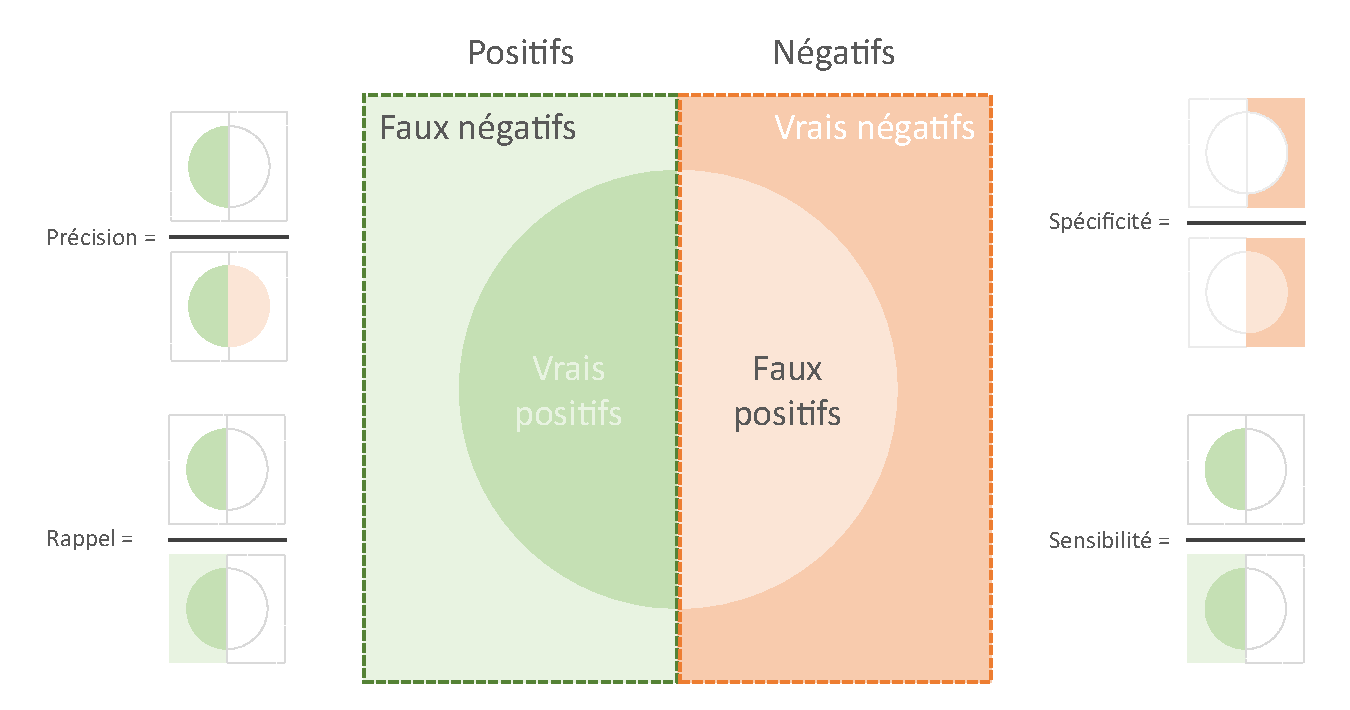
\includegraphics[width=\linewidth]{contents/chapter_3/resources/scheme_confusion_metrics.pdf}
    \caption{Schéma représentatif des principaux métriques obtenues à partir de la matrice de confusion~: la \textit{précision}, le \textit{rappel} ou la \textit{sensibilité} et la \textit{specificité}.}
    \label{fig:scheme_confusion_metrics}
\end{figure}

\begin{equation} 
    \label{eq:metrics_basics}
    \begin{split}
    Sensibilit\acute{e} &= VP/(VP+FN) \\
    Rappel &= Sensibilit\acute{e} \\	
    Sp\acute{e}cificit\acute{e} &=  VN/(VN+FP) \\
    Pr\acute{e}cision &= VP/(VP+FP) \\
    Moyenne &= (VP+VN)/(VP+VN+FP+FN)
    \end{split}
\end{equation}

Dans ce cas, il peut être préférable de privilégier des métriques plus robustes, dans le cadre de données non balancées. La plupart des méthodes s’accordent sur l’utilisation de métriques tels que le \fscore{}, associant conjointement sensibilité et précision, par principe de la moyenne harmonique~\cite{Guo2008}. L'\Cref{eq:metrics_fscore} met à disposition l'expression générique de cette métrique, dont le paramètre $\beta$ permet de moduler l'importance de la précision ou du rappel. L'influence de ce paramètre est neutre lorsque sa valeur est égale à 1 comme dans le cas du \fscore.\par
 
\begin{equation} 
    {F_\beta \: score}=(1+\beta^2)*(Pr\acute{e}cision*Rappel)/((\beta^2*Pr\acute{e}cision)+Rappel)
    \label{eq:metrics_fscore}
\end{equation}
 
Une autre métrique permettant de se prémunir de ces effets de non balancement de l'information et celui de l'\acs{auc} et découlant de la courbe \gls{roc} dont le principe est résumé sur le schéma \Cref{fig:scheme_roc_curve}). La courbe \gls{roc} est tracée à partir des informations de spécificité / sensibilité et par variation d'une valeur seuil appliquée au modèle de prédiction, tandis que l'\gls{auc} correspond à l'intégration de l'aire de cette courbe. Ainsi, l'\gls{auc} est robuste au non-balancement de données mais ses valeurs sont optimistes sur des modèles de prédiction dont la variation du seuil est homogène vis à vis des résultats.\par

\begin{figure}[H]
    \centering
    \includegraphics[width=0.80\linewidth]{contents/chapter_3/resources/scheme_roc_curve.pdf}
    \caption{Schéma de courbe \gls{roc} en orange et \gls{auc} en gris.}
    \label{fig:scheme_roc_curve}
\end{figure}

D'autres alternatives moins biaisées ont également été formulées~\cite{Sokolova2006}. Néanmoins le \fscore{} et l'\gls{auc} sont couramment utilisés dans des articles cliniques et constituent une des bases de ce travail.\par

\clearpage

\subsection{Réglages des hyperparamètres}
\label{subsec:hyperparameter}
Avant d’entrer plus en profondeur dans le sujet, il est nécessaire de revenir sur le terme \textbf{d’hyperparamètres}. Il caractérise les paramètres d'un processus d'apprentissage automatique dont le réglage doit être effectué avant la phase d'entraînement et dont les valeurs dépendent des données à traiter. Le réglage des hyperparamètres peut rarement être déterminé par la simple observation des données, et nécessite ainsi un réglage en fonction de chaque situation rencontrée.\par

L’une des premières techniques permettant ce réglage consiste à définir une \textit{grille} de ces hyperparamètres, contenant pour chacun leurs possibles variations~\cite{Liu2006}. Il s'agit de la méthode la plus équitable puisqu'elle consiste à évaluer chaque combinaison par comparaison des performances finales (voir la \Cref{fig:example_hyperparameter_selection} - Gauche). Néanmoins, elle possède deux limitations majeures, dont~:
\begin{itemize}
    \item son \textbf{temps de calcul}, qui va croître de manière exponentielle en fonction du nombre d'hyperparamètres à valider,
    \item sa \textbf{précision}, qui va dépendre du pas choisi pour chacun des paramètres.
\end{itemize}\par

La seconde technique consiste à définir un \textit{espace} de recherche dont la distribution de chaque hyperparamètre sera choisie, ainsi qu'un nombre d'évaluations à réaliser pour déterminer la meilleure combinaison possible. Ce nombre d'évaluations est ensuite réalisé sous forme de tirage aléatoire, effectué à l'intérieur de cet espace de recherche défini~\cite{bergstra2012} (voir la \Cref{fig:example_hyperparameter_selection} - Droite). Cette méthode possède l'avantage d'être prévisible en termes de temps puisque le nombre de combinaisons évaluées est défini au préalable et quelles que soient les proportions de l'espace. Néanmoins, cette méthode possède également des inconvénients comme la représentation des tirages au sein de l'espace défini.

\begin{figure}[H]
    \centering
    \includegraphics[width=\linewidth]{contents/chapter_3/resources/example_hyperparameter_selection.pdf}
    \caption{Exemple de recherche sur deux hyperparamètres $X_1$ et $X_2$. À gauche, une recherche sous forme de grille rigide, dans laquelle chaque combinaison est évaluée. À droite, une recherche aléatoire de ces hyperparamètres.}
    \label{fig:example_hyperparameter_selection}
\end{figure}

\subsection{Méthodes d'évaluation}
Divers aspects sont évoqués pour permettre l'ajustement des modèles dans la \Cref{subsec:hyperparameter} ainsi que la mesure de leurs performances dans la \Cref{subsec:metrics}. Il est nécessaire d'orchestrer cet ensemble afin d'obtenir la meilleure attente possible d'un modèle de prédiction, tout en conservant une mesure pertinente permettant de renseigner sur la fiabilité de ce modèle et de ses prédictions futures dans des situations où la vérité terrain n'est pas connue. En effet, l'évaluation d'un modèle de prédiction sur des données identiques à celles utilisées constitue un biais, par l'utilisation de connaissances \textit{a posteriori}. De même, l'ajustement des hyperparamètres rentre dans cette catégorie de l'entraînement, et l'évaluation ne peut se faire sur des données ayant servi à les déterminer. Par ailleurs, une telle évaluation permet de détecter les problèmes de sous-apprentissage et sur-apprentissage évoqués en \Cref{subsec:generalized_models}.\par

La méthode \textbf{holdout} est la plus simple d'entre elles et consiste à diviser l’échantillon de données en deux sous-ensembles respectivement d'entraînement et de test. Il est important lors de cette étape de vérifier que les données présentes dans chacun de ces sous-ensembles soient représentatives de chaque classe présente dans la problématique. Les données spécifiées pour le test restent ainsi non utilisées jusqu'à leur confrontation au modèle définitif qui est alors évalué sur ces dernières. Le principal inconvénient de cette méthode est que seule une partie du jeu de données sert d'évaluation à la méthode développée. Néanmoins, cette méthode est rapide à exécuter puisqu'elle ne nécessite l'entraînement que d'un modèle. Cette méthode est schématisée sur la \Cref{fig:scheme_holdout_cv} - Gauche.\par

La méthode de \textbf{validation croisée} permet d'étendre la méthode précédente à l'ensemble du jeu de données et d'obtenir un score moins biaisé. Pour cela, le jeu de données est subdivisé en \textbf{$k$ échantillons}, servant à tour de rôle de jeu de test, le reste de ces données étant réservé à l'entraînement. Ce principe de fonctionnement génère ainsi $k$ modèles de prédictions et autant de scores d'évaluation qui se résument à une unique valeur par application d'une fonction de moyenne. Le principal inconvénient de cette méthode est son temps de réalisation puisqu'elle nécessite l'entraînement d'autant de modèles que d'échantillons. Cette méthode est schématisée sur la \Cref{fig:scheme_holdout_cv} - Droite.\par

\begin{figure}[H]
    \centering
    \includegraphics[width=\textwidth]{contents/chapter_3/resources/scheme_holdout_cv.pdf}
    \caption{Schéma des principes des deux approches majeures d'évaluation de modèles. À gauche, la méthode de \textit{holdout} ; À droite, la méthode de \textit{validation croisée}.}
    \label{fig:scheme_holdout_cv}
\end{figure}

Ce travail s'intéresse à la technique de validation croisée ainsi qu'à la valeur moyenne renvoyée par celle-ci. Afin de rendre cette information plus complète, la valeur de l'écart-type est conjointement calculée à partir des évaluations réalisées sur les divers échantillons, jugée fiable afin de mesurer la stabilité du processus vis-à-vis des données~\cite{Kim2009}. La plupart des travaux ayant recours à la validation croisée emploient une valeur $k$ comprise entre 5 et 10, jugée suffisante pour l'obtention de valeurs de moyenne et écart-type dans un temps de calcul raisonnable~\cite{James2000}. Néanmoins, il est possible d'amener ce principe à l'extrême en choisissant la plus petite valeur possible pour un lot dédié à l'évaluation soit la taille d'une donnée. Cette valeur $k$ devient égale au nombre de données à traiter, devenant un schéma qualifié de \textit{leave-one-out} ou littéralement \textit{en laisser un de côté}. Mais ce type de schéma de validation souffre généralement d'une variance élevée, surtout lorsque les données contiennent des valeurs aberrantes~\cite{Bengio2004}.\par

Ces deux méthodes répondent à la problématique de l'évaluation, mais n'apportent pas de solution quant au choix des hyperparamètres. En effet, utiliser un schéma de validation croisée pour régler et évaluer les modèles conduit inévitablement à surestimer les performances du modèle~\cite{Tsamardinos2014}. Ce type de démarche revient à ajuster au mieux une courbe à un nuage de points tout en affirmant que ces mêmes données correspondent à des données inconnues. L'une des solutions à ce problème est l'utilisation d'un double schéma de validation, dont l'un des plus fonctionnels actuellement est celui de la \textbf{validation croisée imbriquée}~\cite{Cawley2010}. Le principe de cette méthode est schématisé sur la \Cref{fig:scheme_hyperparameter_process}, laquelle se décompose en~:
\begin{itemize}
    \item une boucle \textbf{externe}, permettant d'évaluer un modèle à partir de données de \textbf{test},
    \item une boucle \textbf{interne}, permettant de valider un modèle et ses réglages à partir de données de \textbf{validation}.
\end{itemize}\par
  
\begin{figure}[H]
    \centering
    \includegraphics[width=0.9\linewidth]{contents/chapter_3/resources/scheme_hyperparameter_process.pdf}
    \caption{Schéma de la validation croisée imbriquée assurant le choix de la meilleur combinaison d'hyperparamètres et assurant une évaluation robuste des performances du modèle.}
    \label{fig:scheme_hyperparameter_process}
\end{figure}\par

\clearpage

\section{Fusion d’informations}
\label{sec:fusion_information}
Dernier aspect de ce sujet, la fusion d’informations se définit comme l’action de « combiner des informations issues de plusieurs sources afin d’améliorer la prise de décision »~\cite{Bloch2003}. Cette fusion se retrouve dans de nombreux domaines d'applications dont celui de la santé ou encore de la biométrie, et peut être considérée comme un moyen d'augmenter la fiabilité de systèmes. L'intérêt croissant pour ce domaine correspond, entre autres, à une réponse de l'augmentation et de la diversification du nombre de capteurs présents. L'ouvrage de Bloch~\cite{Bloch2003} justifie la fusion d'informations, par différentes notions auxquelles sont soumises chaque capteur, dont~:
\begin{itemize}
    \item \textbf{l'incertitude}~: c’est-à-dire son « degré de conformité avec la réalité ».
    \item \textbf{l'imprécision}~: définie comme une « mesure du défaut quantitatif de connaissance, sur une mesure ».
    \item \textbf{l'incomplétude}~: correspond à « l'absence d'information d'une source sur des aspects du problème ».
\end{itemize}\par

Cette fusion est indispensable pour permettre la réalisation de certaines tâches, l'effet de McGurk est un exemple concret de la \textit{complémentarité} de la vision et de l'audition dans le rôle de la perception de la parole, mais également de la difficulté à gérer les \textit{conflits} d'informations sur ces deux sources séparées~\cite{Mcgurk1976}. L'ouvrage de Bloch~\cite{Bloch2003} définit trois termes propres à cette fusion~:
\begin{itemize}
    \item \textbf{le conflit}~: l'une des notions pouvant conduire à une mauvaise interprétation du système lorsque plusieurs informations contradictoires sont reçues.
    \item \textbf{la redondance}~: l'apport multiple d'une même information, pouvant dans l'idéal permettre de réduire les incertitudes et les imprécisions.
    \item \textbf{la complémentarité}~: généralement des sources, liée à un apport de caractéristiques différentes permettant l'accès à une information globale et de lever des ambiguïtés.
\end{itemize}\par

Il est nécessaire également de caractériser le résultat de la fusion d'informations. Il est relativement difficile d'obtenir une vision commune sur les divers niveaux et termes associés. Ainsi, ce travail se réfère à l'une d'entre elles~\cite{Dasarathy1997} proche de cette problématique. Trois niveaux de fusion y sont décris~:
\begin{itemize}
    \item le \textbf{niveau bas}, considéré comme étant la fusion sur les données,
    \item le \textbf{niveau moyen}, considéré comme la fusion des caractéristiques ou données plus abstraites,
    \item le \textbf{niveau haut}, considéré comme la fusion des décisions.
\end{itemize} Niveaux au sein desquels le processus de fusion d'informations peut aboutir à~:
\begin{inlinerate}
    \item une sélection,
    \item une transformation,
    \item une extraction,
    \item ou encore une classification de l'information.
\end{inlinerate} La \Cref{fig:scheme_overview_fusion} propose une schématisation macroscopique de ce concept.\par
 
\begin{figure}[H]
    \centering
    \includegraphics[width=\linewidth]{contents/chapter_3/resources/scheme_overview_fusion.pdf}
    \caption{Schéma des différents niveaux théoriques de fusion sur un schéma multimodal à deux capteurs. Le niveau bas représente le niveau le plus proche des données et des capteurs, le niveau moyen représente le niveau au plus proche de l'extraction de caractéristiques avancées, enfin le niveau haut représente le niveau de prise de décision.}
    \label{fig:scheme_overview_fusion}
\end{figure}\par

La fusion à \textbf{bas niveau} s'exerce au niveau du capteur, quand celui-ci bénéficie de plusieurs relevés d'informations physiques, ou après l'acquisition de données provenant de plusieurs capteurs. Cela va nécessiter une cohérence entre ces modalités~: un référentiel, un repère commun permettant la mise en parallèle de ces dernières. La fusion à ce niveau consiste essentiellement à fournir une cohérence de ces modalités d'information, voire à réduire cette dernière afin de n'obtenir que celle jugée pertinente dans le cadre de son utilisation.\par

La fusion à \textbf{moyen niveau} s'exerce au niveau de caractéristiques, c’est-à-dire après un premier traitement de chacune des modalités pour n'extraire que les éléments nécessaires à la réalisation du processus. Il s'agit d'une mise en commun des vecteurs d'information dans leur totalité ou réduite nécessitant dans ce second cas une sélection de l'information pertinente.\par

Enfin, la fusion à \textbf{haut niveau} s'exerce après les mécanismes de prise de décision. C’est-à-dire que les branches correspondant à chaque modalité exercent indépendemment leur prise de décision. Il est donc nécessaire de définir une stratégie permettant de privilégier une décision ou d'extraire une décision à partir de l'information. Deux catégories sont ainsi identifiables~: 
\begin{inlinerate}
    \item la \textbf{sélection dynamique de modèle} de prédiction dans lequel l'objectif est de définir le modèle pertinent,
    \item et la \textbf{fusion de modèles} de prédiction dans lequel le but est d'obtenir une décision globale tenant compte des différentes décisions.
\end{inlinerate}\par

Plus particulièrement, dans le cadre de problématique binaire, la fusion de modèle comporte deux niveaux conceptuels de décision basés sur le type d'information mise à disposition par ces modèles. D'une part, au plus haut niveau~: la fusion appliquée au \textbf{niveau décisionnel}. Seules les décisions issues de chaque modèle sont alors considérées selon diverses stratégies~: le vote à la majorité ou encore la pondération des votes en sont deux représentants. D'autre part, au plus bas niveau~: la fusion appliquée aux scores~\cite{Kittler1998}. Dans le cadre de problématiques à plusieurs classes, il est possible possible d'évoquer une troisième prise de décision au niveau du rang, c’est-à-dire en considérant la position de chaque classe prédite issue des divers modèles.\par


% \subsection{Équilibrage de données}
% Nous regroupons au travers de ce terme l’ensemble des problématiques relatives à notre jeu de données et à la représentation de ses classes. Dans le cas de pathologie de la peau, cela peut se caractériser par un jeu de données composé de 100 éléments dont 20~\% d’entre elles se réfèrent à des patients atteints de mélanomes et le reste à des patients sains. Nous constatons dans ce cas un déséquilibre entre les classes de ce jeu de données, qu’il nous faudra prendre en compte. Un tel jeu de données peut être qualifié de « non balancés », la répartition de ses classes n’étant pas égale en proportions.
% En effet, certains algorithmes de prédictions peuvent être biaisés, comme par exemple « l’algorithme des plus proches voisins » qui se composera de zones de forte densité privilégiant les données présentes en masse (exemple Figure 37). Un autre biais est également présent lors de l’extraction de métriques pour juger de la pertinence d’un modèle. En effet, dans le cas d’un classifieur qui prédirait constamment « sain », nous obtiendrons un score de 80~\% de précision sur notre jeu de données précédent.
  
% \begin{figure}[H]
%     \centering
%     \includegraphics[width=\linewidth]{contents/chapter_3/resources/unbalanced.pdf}
%     \caption{Illustration du problème de données non balancées sur l’algorithme KNN. La densité des données bleu étant supérieure, des prédictions à la frontière de nos deux classes favorisent la classe bleue.}
%     \label{fig:unbalanced}
% \end{figure}

% Plusieurs méthodes existent dans la littérature, pour permettre de rétablir l’équilibre entre les différentes classes. Nous pouvons citer les deux principaux~:
% 	Le sur-échantillonnage, c’est-à-dire que nous gonflons les classes sous représentatives de manière à égaliser la population de la classe majoritaire (en créant de nouveaux éléments artificiels par exemple).
% 	Le sous-échantillonnage, c’est-à-dire que nous réduisons la population de l’ensemble des classes à celle de la classe minoritaire.
 
% \begin{figure}[H]
%     \centering
%     \includegraphics[width=\linewidth]{contents/chapter_3/resources/example_balancement_strategies.pdf}
%     \caption{Représentation de deux principales catégories de stratégie de balancement des données. Le suréchantillonnage tente d’augmenter la taille du jeu de données faible tandis que le sous échantillonnage tend à réduire la classe majoritaire. }
%     \label{fig:example_balancement_strategies}
% \end{figure}
% \renewcommand{\thechapter}{\roman{chapter}}
% \setcounter{chapter}{2}
% \unchapter{Epilogue - Données de travail}

\chapter{Données de travail et littérature}
\label{chap:chapter_31}
\chapterintro

Nous traiterons au sein de cette partie de notre "matière" de travail. En effet, l'ensemble de ce travail prend appui sur une base de données mise à disposition initialement pour la réalisation d'une étude clinique menée sur la pertinence de la dermoscopie et de la \gls{rcm} en milieu clinique~\cite{Cinotti2018}. Ainsi, nous débuterons par une présentation de l'étude clinique en décrivant les conditions d'inclusions des patients, les dispositifs d'acquisition et le protocole d'évaluation des experts. Puis, nous étudierons en détail les résultats obtenus par ces experts qui nous servirons de repère dans cet étude. Enfin, nous aborderons des aspects de structuration de la base nécessaire à son utilisation dans le reste de ce document.\par

Cette base a reçu une autorisation de la part du comité d'éthique du \gls{chu} de Saint-Etienne pour son exploitation au sein de l'étude clinique mentionnée précédemment mais également pour ce travail universitaire (Numéro du comité d'examen institutionnel 672016/CHUSTE).\par

Cette base de données compile des lésions faciales possédant les critères suivants :
\begin{itemize}
\item les images proviennent de patients inclus entre les années 2011 et 2015 au \gls{chu} de Saint-Etienne (monocentrique),
\item les données sont disponibles pour chaque patient sous 3 formes que sont la photographie clinique, la dermoscopie et la \gls{rcm} (multimodales),
\item les lésions considérées cette base sont celles dont le diagnostic différentiel, c'est à dire par élimination méthodique des causes (voir
\Cref{subsec:lentigo}), était fortement controversé et supposé comme étant un \gls{lm} ou \gls{lmm}.
\end{itemize}\par

En terme de composition, la base regroupe 201 patients répartis entre 96 femmes et 105 hommes d'un âge moyen égal à 70 ans compris entre 29 et 97 ans comme présenté sur la \Cref{fig:statistics}. Cette base comporte 223 lésions uniques dont le diagnostic que nous utiliserons comme référence provient de l'histologie. Ces lésions se décomposent en :
\begin{itemize}
\item 115 malignes : scindée en 92 \gls{lm} et 23 \gls{lmm}
\item 108 bénignes : dont 20 \gls{bcc}, 37 \gls{sl}, 23 \gls{sk}, 15 \gls{pak}, 8 nævus, 2 kératoses lichénoïde, 2 cicatrices et 1 maladie de Bowen pigmentée.
\end{itemize}\par

\begin{figure}[H]
    \centering
    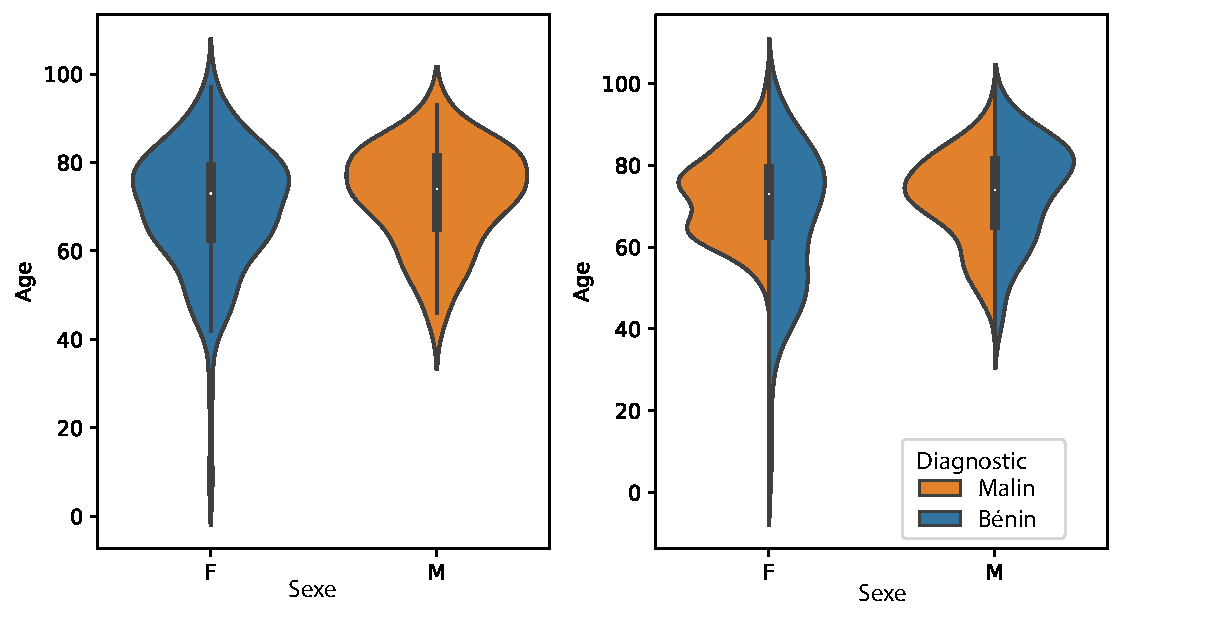
\includegraphics[width=0.8\linewidth]{contents/chapter_2/resources/statistics_age_sex.pdf}
    \caption{A gauche, répartition en fonction de l'âge et du sexe. A droite, répartition entre l'âge et le sexe en tenant compte du diagnostic binaire.}
    \label{fig:statistics}
\end{figure}\par

En ce qui concerne leur acquisition, celle-ci a été à chaque fois réalisée par l'un des 3 experts investigateurs de l'étude clinique~\cite{Cinotti2018}. Tout cas de collisions de tumeurs au sein d'un même groupe a été exclu de cette étude. En ce qui concerne la modalité de dermatoscopie, les données ont été produites à l'aide d'une caméra PowerShot® G7~\textsuperscript{\ref{footnote:device_powershot}} couplée au dispositif proposé par Fotofinder~\textsuperscript{\ref{footnote:device_fotofinder}}. Pour ce qui est de la modalité de \gls{rcm}, les données proviennent d'un VivaScope 3000®~\textsuperscript{\ref{footnote:device_mavig}}. En revanche, aucune information liée à l'acquisition des données de photographie clinique n'a été mentionnée.\par

L'intérêt de ces trois modalités est grand dans le contexte de la dermatologie puisqu'elles représentent le processus "classique" de prise en charge clinique, de la modalité la moins onéreuse avec la \textbf{photographie clinique} mais également la moins précise, à des modalités plus onéreuses, également plus riche en information, avec la \textbf{\gls{rcm}}. Ainsi, chaque modalité permet de réduire ainsi la zone d'incertitude chez un patient souffrant d'une pathologie de la peau.

\addtocounter{footnote}{1}
\footnotetext[\thefootnote]{Source : Canon Powershot®, Canon, Tokyo, Japon. \label{footnote:device_powershot}}
\addtocounter{footnote}{1}
\footnotetext[\thefootnote]{Source : FotoFinder Systems GmbH, Bad Birnbach, Allemagne. \label{footnote:device_fotofinder}}
\addtocounter{footnote}{1}
\footnotetext[\thefootnote]{Source : Distribué en Europe par MAVIG GmbH, Munich, Allemagne. \label{footnote:device_mavig}}

Afin d'évaluer les performances de praticiens face à ces lésions, les investigateurs ont eu recours à 21 dermatologues détenant une expertise des modalités d'imagerie non invasives. Ces experts sont répartis de manière homogène selon leurs compétences respectives pour chacun des dispositifs. Ainsi, le panel d'évaluation se décompose de la façon suivante: 
\begin{inlinerate}
\item 6 experts sont soumis à l'ensemble des modalités,
\item 15 experts sont soumis à l'évaluation de la photographie clinique et de la dermoscopie (dont 9 uniquement dédiés a ces deux modalités),
\item et 12 sont soumis à la \gls{rcm} (dont 6 uniquement dédiés à la \gls{rcm})~\cite{Cinotti2018}.
\end{inlinerate}
Cette répartition est résumée en \Cref{fig:experts_evaluation}. Pour chaque cas clinique étudié, ces experts ont évalué la gravité du cas à l'aide des termes bénin et malin.\par

\begin{figure}[H]
    \centering
    \includegraphics[width=0.6\linewidth]{contents/x_clinical_data/resources/experts_evaluation.pdf}
    \caption{Répartition du panel de 21 dermatologues sur l'évaluation des diverses modalités~\cite{Cinotti2018}.}
    \label{fig:experts_evaluation}
\end{figure}\par

Pour éviter tout biais dans l'évaluation, les experts évalués sur l'ensemble des modalités ont été sollicités sur trois journées différentes: 
\begin{inlinerate}
\item une première évaluation ne comprenant que les images de photographie clinique et de dermoscopie,
\item une seconde évaluation ne comprenant que les images de \gls{rcm}
\item et une dernière évaluation sur l'ensemble de la base d'images.
\end{inlinerate}
Par ailleurs, les cas cliniques ont été présentés dans un ordre différents entre chaque journée d'évaluation afin d'éviter des biais liés à l'activité précédente des experts.\par

% \subsection{Résultats des experts}

Afin de réaliser nos divers tests, une base d'images anonymisée nous a été remise, composée :
\begin{itemize}
\item d'un fichier tableau de lésions comprenant:
    \begin{inlinerate}
        \item en colonne, les diverses informations: \textit{Âge, Sexe,	Zone, Côté,	Diagnostic Binaire et Diagnostic},
        \item en ligne, les divers enregistrement liée à chaque lésion.
    \end{inlinerate}
    \item d'un répertoire comprenant les images des divers cas clinique recensés dans l'étude sous divers formats image.
\end{itemize}\par

Afin d'exploiter au mieux cette base, quelques modifications y sont apportées. D'une part, la diversité des formats images est un frein quand à la gestion de ces données et nous avons opté pour un format matriciel sans perte de type bitmap. D'autre part, la structure de la base ne permet pas l'utilisation d'annotation au niveau des images ou des instances autres. Afin de rendre plus dynamique cette partie, nous avons opté pour une structure reprenant le fichier table initial (au format \gls{csv}) et de répertoires associés à chaque lésion. Chaque dossier de lésion se compose lui même de fichiers d'annotation propre au type de données stockées (images ou patchs). Par ailleurs, certains apports d'informations ont été réalisés pour permettre un bon déroulement de la suite de notre travail, tel que l'appartenance à un patient. La \Cref{fig:db_structure} synthétise la structure de cette base avant et après modification.\par

\begin{figure}[H]
\centering
    \begin{subfigure}{.45\textwidth}
      \centering
      \includegraphics[width=\linewidth]{contents/x_clinical_data/resources/scheme_dbstructure_old.pdf}
    \end{subfigure}
    \begin{subfigure}{.45\textwidth}
      \centering
      \includegraphics[width=\linewidth]{contents/x_clinical_data/resources/scheme_dbstructure_new.pdf}
    \end{subfigure}
    \caption{Schéma de l'organisation de la base de ressources employée. A gauche, la base initiale et à droite, la base restructurée afin de supporter de nouvelles annotations.}
    \label{fig:db_structure}
\end{figure}\par

% Part 2
\part{Microscopie confocale par réflectance}
\label{part:microscopie}
\renewcommand{\thechapter}{\roman{chapter}}
\setcounter{chapter}{3}

\unchapter{Préambule microscopie confocale par réflectance}
\label{chap:preamble_microscopy}
Pour permettre l'identification de pathologie en dermatologie plus routinière, la mise en avant de critères de diagnostic est une démarche clé permettant de rendre cette tâche plus efficace. Cette mise en avant de critères à été débutée au milieu des années 1980, sous la forme:
\begin{itemize}
    \item d'\textbf{acronyme}: l'idée est de proposer une méthode de diagnostic facile à mémoriser. Le travail de Friedman est un exemple, bien que révisé, le critère ABCD(E) est encore utilisé et applicable par de nombreuses personnes expertes ou non~\cite{Friedman1985}.
    \item de \textbf{liste}: de critères positifs et négatifs, correspondant à des caractéristiques rédhibitoires ou non, et amenant à un score final. Ce score variera selon la pathologie considérée et permettra d'en déduire une décision à prendre. L'un des exemple dans le cadre de lésions pigmentées est celui de MacKie en 1986~\cite{mackie1986}. Ces critères ont été révisés et se destinent néanmoins à un public expert. 
\end{itemize}\par

Ces démarches "algorithmiques" de diagnostic, ainsi nommés, se sont progressivement étendues à d'autre pathologies et dispositifs d'analyse médicaux. Ils permettent de se référer à des critères essentiels en cas de doute. Le \gls{rcm} n'est pas exempt de ces démarches simplifiées, notamment pour la démarche du \gls{lm} avec les travaux de Pellacani et Guitera~\cite{Pellacani2007, Guitera2010}. Ces deux travaux proposent sous forme de table de critères ceux jugés positifs et négatifs, dont la \Cref{tab:rcm_algorithm_lentigo} donne un aperçu de la production de ces articles. Leur étude comptabilise 81 cas de \gls{lm} et 203 lésions bénignes, sur lesquels un seuil de score de 2 à été jugé comme pertinent en regard de l'étude statistique menée. Celui-ci à permis de détecter avec 85\% de sensibilité et 76\% de spécificité les \gls{lm}.\par

\begin{table}[H]
\centering
\begin{tabular}{ll}
\toprule
Type de caractéristiques                        & Caractéristiques                                              \\\hline
\multirow{2}{*}{Positives Majeures (+2 points)} & Papilles à contour faiblement définis                         \\\cline{2-2}
                                                & Cellules pagétoides rondes >\SI{20}{\micro\metre}             \\\hline
\multirow{3}{*}{Positives Mineures (+1 points)} & Présence de cellules atypiques dans la \gls{dej}              \\\cline{2-2}
                                                & Combinaison de follicule et cellules atypique et/ou pagétoide \\\cline{2-2}
                                                & Présence de cellules nucléée au sein de papilles              \\\hline
Négatives Mineures (-1 points)                  & Motif en alvéoles larges                                      \\
\bottomrule
\end{tabular}
\caption{Caractéristiques observables par \gls{rcm} jugées pertinentes par l'étude de Guitera et Pellacani pour la détection du \gls{lm}~\cite{Guitera2010}.}
\label{tab:rcm_algorithm_lentigo}
\end{table}\par
 
De manière plus détaillé, ces caractéristiques ont été qualifiées comme pertinente par leurs auteurs~\cite{Pellacani2007, Guitera2010}, lorsque une propriété était significativement plus présente dans l'un des deux groupes pathologique (\gls{lm} ou bénin). L'un de ces travaux~\cite{Guitera2010} procède à une analyse par profondeur de ces caractéristiques. Les éléments majeurs de cette étude sont listés ici, selon une profondeur croissante:
\begin{itemize}
    \item au niveau de \textbf{l'épiderme}, les auteurs ont constaté que les pathologies de \gls{lm} comportent un désordre des cellules de l'épiderme (56\% des lésions \gls{lm} contre 18\% des lésions bénignes). Également, une infiltration pagétoïde a été reportée dans la plupart des cas de \gls{lm}  (75\% des lésions \gls{lm} contre 28\% des lésions bénignes). En opposition, un épiderme homogène, caractérisé part des motif en nids d'abeille, ont été constatés dans 92\% des cas bénins \Cref{fig:example_rcm_pattern_1}.
    \item au niveau de la \textbf{\gls{dej}}, les auteurs ont constaté que les papilles non démarquée étaient observées dans la majorité des \gls{lm} (68\% \gls{lm} and in 17\% des cas bénins) \Cref{fig:example_rcm_pattern_2}.
    \item au niveau du \textbf{derme}, 15\% des cas de \gls{lm} présentent des cellules nuclées large contre 2\% des lésions bénignes \Cref{fig:example_rcm_pattern_3}.
\end{itemize}\par

\begin{figure}[H]
    \begin{center}
        \includegraphics[width=0.9\linewidth]{contents/x_microscopy/resources/example_rcm_pattern_1.pdf}
        \caption{Cas de données cliniques \gls{rcm} en provenance de l'épiderme par Guitera~\cite{Guitera2010}. En a) et b), exemples de motifs en large nids d'abeille (\textit{broadened honeycomb pattern}), respectivement d'un kératose séborrhéique et de peau normale; en c), exemples de motifs de pavés atypiques (\textit{atypical cobblestone pattern}) issue d'un \gls{lm}; en d), exemples de \textit{large pagetoid} cellules propre au \gls{lmm}. Repère : barre = \SI{50}{\micro\metre}.}
        \label{fig:example_rcm_pattern_1}
    \end{center} 
\end{figure}\par

\begin{figure}[H]
    \begin{center}
        \includegraphics[width=0.7\linewidth]{contents/x_microscopy/resources/example_rcm_pattern_2.pdf}
        \caption{Cas de données cliniques \gls{rcm} par Guitera~\cite{Guitera2010}. En a) et au niveau de la flèche, exemple de papille à frontière non marqué (\textit{Nonedge papillae}) et de cellules atypique d'un \gls{lm} acquise à la jonction \gls{dej}; En b), exemple de papilles à frontières marquées (\textit{Edge papillae}) d'une pathologie bénigne. En c), exemple de cellules atypiques au niveau de la \gls{dej} typique de \gls{lm}; En d), exemple de halo noir autour de celulles atypiques de l'épiderme issue d'un \gls{lm}. Repère : barre = \SI{50}{\micro\metre}.}
        \label{fig:example_rcm_pattern_2}
    \end{center} 
\end{figure}\par

\begin{figure}[H]
    \begin{center}
        \includegraphics[width=0.8 \linewidth]{contents/x_microscopy/resources/example_rcm_pattern_3.pdf}
        \caption{Cas de données cliniques \gls{rcm} par Guitera~\cite{Guitera2010}. En a), exemple de cellules atypiques à proximité d'un follicule pileux au sein de la \gls{dej} sur un un \gls{lm}; En b), exemple de cellules nucléé du derme d'un \gls{lm}. Repère : barre = \SI{50}{\micro\metre}.}
        \label{fig:example_rcm_pattern_3}
    \end{center} 
\end{figure}\par

Dans l'étude menée par Cinotti~\cite{Cinotti2018}, les auteurs investigateurs ont demandés d'évaluer certaines caractéristiques récurrentes de la littérature. Parmis lesquelles:
\begin{itemize}
    \item Large roundish pagetoid cells. LM 37% (range 9-70%, SD 20), B 5% (range 1-13%, SD 4)
    \item large dendritic cells in the epidermis LM 81% (range 66-91%, SD 9), B  13% (range 8-20%, SD 4)
    \item follicular localization of atypical cells LM 62% (range 55-75%, SD 8), B 7% (range 3-11%, SD 2)
\end{itemize}\par

\begin{figure}[H]
    \begin{center}
        \includegraphics[width=\linewidth]{contents/x_microscopy/resources/scheme_rcm_statistics.pdf}
        \caption{Répartition de nos annotation au niveau des images (à gauche) mais également sur les patchs (à droite).}
        \label{fig:scheme_rcm_statistics}
    \end{center} 
\end{figure}\par

Les données \gls{rcm} de chaque lésions contiennent essentiellement des images jugées pertinentes par deux des trois médecins investigateurs et provenant de l'épiderme, de la \gls{dej} et du derme. Néanmoins, les données utilisées ici correspondront essentiellement à des données de la \gls{dej}. En effet, le \gls{lm}/\gls{lmm} sont des pathologies de la peau caractérisées par l'intrusion de de la mélanine se propageant le long des follicules pileux. Les images de la \gls{dej} sont ainsi parfaitement adaptées à l'observation de ce phénomène par les médecins. \par

Du point de vue de leurs caractéristique ces images arborent une taille constante de \SI{1000}{\px} $\times$ \SI{1000}{\px} pour une section mesurée de \SI{920}{\micro\metre} $\times$ \SI{920}{\micro\metre} pour une résolution axiale comprise entre \SIrange{3}{5}{\micro\metre}. Ces données fournissent ainsi une résolution de l'ordre du \SI{1}{\micro\metre}. De plus, aucune méta information ne pourra être utilisée pour traiter cette problématique, les quelques information étant pour la plupart erronée: procédure de calibration non réalisée, informations manquante, mode d'imagerie différents.\par

Pour finir, l'objectif visé par cette partie sera l'évaluation de technique d'imagerie sur la qualité du diagnostic sur base d'images issues de \gls{rcm}. A ce titre nous ne nous reposerons pas sur les méta données issues des informations patient: l'âge, le sexe ou encore l'emplacement seront autant de critères que nous ne considérerons pas au sein de ces prochains paragraphes bien que ceux ci soient utilisés par les dermatologues experts en \gls{rcm} durant leur évaluation~\cite{Cinotti2018}.\par

\begin{figure}[H]
    \begin{center}
        \includegraphics[width=\linewidth]{contents/x_microscopy/resources/example_rcm_data.pdf}
        \caption{Exemple de tissus.}
        \label{fig:example_rcm_data}
    \end{center} 
\end{figure}\par


Concernant l'étude de référence~\cite{Cinotti2018}, 
\begin{figure}[H]
    \begin{center}
        \includegraphics[width=\linewidth]{contents/x_preamble_microscopy/resources/results_rcm_experts.png}
        \caption{.}
        \label{fig:results_rcm_experts}
    \end{center} 
\end{figure}\par


Au sein de ce premier chapitre, nous élaborerons une méthodologie destinée à la modalité \gls{rcm}. Les éléments nous ayant conduit à nous intéresser à cette modalité sont multiples. En premier lieu, il s'agit de l'une des modalités les plus précise en notre possession, elle consiste donc en une référence en terme de qualité de diagnostic à réaliser. Enfin, le nombre restreint de travaux menée sur le diagnostic de lésion de la peau appliqué au \gls{rcm} assisté par ordinateur est un second argument. En effet, cette modalité représente pour nous un verrou scientifique nous devons lever pour accomplir le schéma de diagnostic multimodal.\par

Pour cela, nous sollicitons diverses ressources d'intelligence artificielle évoquées lors de précédent chapitre. De plus, certains ajouts ont été réalisés pour permettre le déroulement des expériences suivantes. En effet, la base d'image actuelle ne possède que des annotations au niveau des patients, ce qui limite fortement nos travaux.
A l'aide d'un outil graphique réalisé pour cette étude (\Cref{fig:example_gui_annotation}, nous avons pu obtenir grâce au travail de l'un des dermatologistes investigateur:
\begin{itemize}
\item des annotations au niveau des images,
\item des annotations au niveau de sous parties d'images ou \textbf{patchs}.
\end{itemize}\par

\begin{figure}[H]
\centering
    \begin{subfigure}{.45\textwidth}
      \centering
      \includegraphics[width=0.8\linewidth]{contents/x_preamble_microscopy/resources/example_gui_annotation_1.png}
    \end{subfigure}
    \begin{subfigure}{.45\textwidth}
      \centering
      \includegraphics[width=0.8\linewidth]{contents/x_preamble_microscopy/resources/example_gui_annotation_2.png}
    \end{subfigure}
    \caption{Interface logicielle mise à disposition du spécialiste, afin de procédé aux annotations. A gauche, l'onglet permettant l'annotation au niveau des images, à droite l'onglet permettant la création de patchs.}
    \label{fig:example_gui_annotation}
\end{figure}

Ainsi, dans cette partie ne seront considérée que les données \gls{rcm} des 223 lésions en notre possession et seront donc exclues images de photographie clinique et dermatoscopie. Également, ont été utilisés 28 patient bénins non présent dans la base d'image initiale afin d'augmenter le nombre d'images annotées comme bénignes. Ces images comportent également des lésions pouvant porter à préjudice lors du diagnostic de \gls{lm}/\gls{lmm}. Ces données ne seront utilisées uniquement dans le but de renforcer l'entraînement. La répartition complète de cette base peux être visualisé en \Cref{fig:scheme_rcm_statistics}.\par


Afin de répondre à ce besoin, cette partie dédiée au \gls{rcm} se compose de trois chapitres dans lesquels nous élaborerons une méthodologie ascendante:
\begin{inlinerate}
\item le premier chapitre abordera la \textbf{prise de décision au niveau de l'image},
\item le second chapitre proposera des \textbf{perspectives d'amélioration},
\item enfin le dernier chapitre de cette section se focalisera sur une \textbf{prise de diagnostic au niveau du patient}.
\end{inlinerate}\par
\newpage
\chapter{Diagnostic de l'image}
\label{chap:chapter_4}
\chapterintro
Comme évoqué durant le préambule, cette partie s'intéresse au premier niveau de diagnostic, c'est à dire celui de l'image sur données \gls{rcm}. La séparation sur problématique binaire, malin et non malin, sera ainsi évaluée mais également sur trois classes avec d'une part les tissus sains, bénin et malin.\par

Ainsi, plusieurs aspects se distinguerons dans ce chapitre dont l'extraction de caractéristiques pertinentes par méthodes manuelles et auto déterminée et l'utilisation de méthodes de classification éprouvées. Nous nous intéresserons également à l'influence de divers paramètres liés à la normalisation des caractéristiques, à la réduction de l'information dans le cadre des méthodes sur base d'apprentissage par transfert et enfin sur l'influence des données sur les résultats obtenus.\par	
\newpage

%%%%%%%%%%%%%%%%%%%%%%%%%%%%%%%%%% 
%%%%%%%%%%%%%%%%% METHODOLOGIE
\section{Méthodologie}
La classification de la peau par méthode d'apprentissage est un problème très largement développée dans la littérature, notamment pour le mélanome. Néanmoins, dans le cadre de la détection du \gls{lm}/\gls{lmm} sur base d'images \gls{rcm},
cette problématique n'a été abordé que par quelques articles~\cite{Halimi2017a, Halimi2017b, Wiltgen2008, Koller2011}. Nous nous intéresserons à la détection de cette pathologie au sein de la base d'image mise à disposition, et nous étudierons cette problématique selon divers angles d'approche: 
\begin{inlinerate}
    \item la séparation entre les tissus malin et le reste des tissus (problématique à 2 classes),
    \item la séparation entre les tissus pathologiques  et les tissus qualifiés de sains (problématique à 2 classes),
    \item et enfin la séparation des tissus malins, bénins et sains (problématique à 3 classes).
\end{inlinerate}\par

Afin de traiter ces problématiques, nous aborderons ces cas à l'aide de mécaniques liées à l'apprentissage supervisé, que nous déroulerons lors de prochains paragraphes. En effet, ces mécaniques ont largement été employé et démontrée fonctionnelles dans des problèmes similaires de classification d'images médicales. Dans un premier temps, nous décrirons le processus par apprentissage automatique ( voir \Cref{fig:scheme_macro_pipeline} - en haut): nous décrirons bloc par bloc les traitements proposés de l'extraction de caractéristique à l'étape de classification. Dans un second temps, nous décririons le processus d'apprentissage profond ( voir \Cref{fig:scheme_macro_pipeline} - en bas): nous traiterons de l'augmentation des données et proposerons une méthodologie d'entraînement. Enfin, nous terminerons par une descriptions des résultats obtenus, tenterons d'expliquer ces derniers, et déterminerons les choix les plus cohérents pour la suite.\par

\begin{figure}[H]
\centering
    \includegraphics[width=\linewidth]{contents/chapter_4/resources/scheme_macro_pipeline_machine.pdf}
    \caption{Représentation macroscopique du processus de diagnostic image suivi dans le cadre de l'apprentissage automatique.}
    \label{fig:scheme_macro_pipeline}
\end{figure}\par

Cette section se destine à présenter l'ensemble des étapes consacrée à la classification des images de \gls{rcm} selon un processus d'apprentissage automatique. Celui-ci se décompose en quatre étapes majeures:
\begin{inlinerate}
    \item l'extraction de caractéristiques,
    \item le balancement des données,
    \item le post-traitement,
    \item et la classification
\end{inlinerate}.
Le pré traitement des images n'est pas considéré car jugé peu utile sur ces dernières. Ce processus sera décrit point par point lors des prochaines sous-parties.\par
\newpage

%%%%%%%%%%%%%%%%%%%%%%%%%%%%%%%%%% 
%%%%%%%%%%%%%%%%% FEATURES
\section{Extraction de caractéristiques}
\label{chap:feature_extraction}
L'étape d'extraction de caractéristiques consiste en l'obtention de valeurs dérivées à partir des données brute dans le but de quantifier un phénomène jugée pertinent pour la suite du traitement (généralement de la classification). Les éléments présentés en \Cref{chap:preamble_microscopy} portent à montrer l'importance des motifs de tissus, très variables selon:
\begin{itemize}
    \item la profondeur d'acquisition : l'épiderme, \gls{dej} et le derme sont très différents du point des tissus,
    \item la pathologie à identifier : les différentes lésions en notre possession sont assez différentes selon leur états bénin ou malin.
\end{itemize}\par

Les nombreux échanges menés auprès des spécialistes en dermatologie ont également abouti sur une importance des aspects des textures au sein de leur processus cognitifs de décision vis à vis des pathologies de \gls{lm}/\gls{lmm}.\par

Nous traiterons des techniques d'extraction de caractéristiques appliquée à notre thématique, que nous aborderons selon deux axes:
\begin{inlinerate}
    \item d'une part les techniques d'extraction de caractéristiques manuelles,
    \item d'autre part les techniques d'extraction de caractéristiques non manuelles
\end{inlinerate}. Ces termes ont été utilisés suite à l'apparition de réseaux de convolution profonds, afin de catégoriser ces deux types d'approches~\cite{Nanni2017}.\par

L'extraction de caractéristiques est une problématique qui a été traitées sous deux aspects distincts: l'une par utilisation du domaine spatial et l'autre par utilisation du domaine fréquentiel. Ainsi, ces prochaines lignes traiterons la problématique dans cet ordre respectif.\par

\subsection{Extraction de caractéristiques manuelles spatiales}
L'extraction sur base d'information du domaine spatial est un champs de travail assez développé présentant comme avantage d'être intuitif mais pouvant être affecté par le bruit et distorsions. Ces opérations spatiales peuvent être décrites à deux niveaux: les descripteurs de premier ordre ne prenant en compte que les valeurs d'intensités initiales et est indifférent aux information de voisinage; et les descripteurs de second ordre et plus, prenant en compte la relation d'une valeur locale et de son voisinage~\cite{Kamila2015}.\par

Les descripteurs de premier ordre s'appliquent ainsi aux valeurs d'intensité ou à la distribution de celle-ci, sans traitement préalable. La \Cref{tab:first_order_descriptors} recense la plupart des ces mesures. Néanmoins, ces mesures tendent à ressortir des phénomènes globaux de l'image mais ne suffisent pas à elles seules à analyser  des motifs présent, mais peuvent constituer un bon complément ~\cite{Tomita1990, Srinivasan2008, Uyun2013, NyeinNyeinHlaing2015}.\par

\begin{table}[H]
    \centering
    \begin{tabular}{ll}
        \toprule
        \textbf{Mesure}             & \textbf{Formule}                                                              \\ \hline
        Moyenne                     & $\overline{x} = {1 \over n} \sum_{i=1}^n{x_i}$                                \\   
        Variance                    & $\overline{x} = \frac{1}{n}\sum_{i=1}^n x_i$                                  \\ 
        Entropie                    & \\
        Kurtosis (Courbure)         & \\
        Asymétrie                   & $\gamma_1 = \mathbb{E} \left[ \left( \frac{X - \mu}{\sigma} \right)^3 \right]$\\  
        \bottomrule
    \end{tabular}
    \caption{Liste de différentes mesures obtenues à partir du premier ordre.}
    \label{tab:first_order_descriptors}
\end{table}\par

Les descripteurs de second ordre, ou plus, utilisent l'information locale et en déduisent une relation à leur voisinage par l'utilisation généralement d'une transformation intermédiaire. Parmi ces transformation, les plus courantes sont: 
\begin{inlinerate}
    \item \gls{glcm},
    \item \gls{glrlm},
    \item et \gls{glszm}.
\end{inlinerate} 
L'extraction sur la base d'information du second ordre à notamment été traitée en 1973 pour de la reconnaissance d'image aérienne et satellites, par Robert Haralick~\cite{Haralick1973}. Ce travail est une extension des \gls{glcm}, dont le principe consiste en un recensement des combinaisons d'intensité présentent dans une image. Cette extraction nécessite une direction dans laquelle les combinaisons seront recherchées, en 2D ces directions sont aux nombre de quatre:
\begin{inlinerate}
    \item horizontale,
    \item verticale,
    \item et les deux diagonales opposées
\end{inlinerate}. Le principe de fonctionnement des \gls{glcm} est schématisé en \Cref{fig:scheme_principle_GLCM} pour une extraction selon la direction horizontale. Le travail~\cite{Haralick1973} à ainsi démontré la pertinence des \gls{glcm} dans la différenciation d'images texturés, en calculant quatorze critères statistiques selon les quatre directions évoqué précédemment. La \Cref{tab:haralick_descriptors} met à disposition les diverses mesures utilisées et formules associées. Afin de réaliser ces diverses extraction de manière optimum, nous nous référé à la bibliothèque logicielle "Mahotas"~\cite{coelho2012} proposant ces diverses mesures de manière optimisée.\par
 
\begin{figure}[H]
    \centering
    \includegraphics[width=0.8\linewidth]{contents/chapter_4/resources/scheme_principle_GLCM.pdf}
    \caption{Représentation de la création d'une matrice sur base de \gls{glcm} selon la direction horizontale.}
    \label{fig:scheme_principle_GLCM}
\end{figure}\par

L'un des travaux menée par une étude sur les lésions mélanocytaire en \gls{rcm} vont dans le sens de ces deux formes d'information~\cite{Wiltgen2008}. En effet, l'étude met en avant l'importance des douze première caractéristiques énoncés par Haralick et adjoint cinq mesure de premier ordre comme complément d'information dont :
\begin{inlinerate}
    \item la moyenne,
    \item l'erreur quadratique moyenne,
    \item l'asymétrie de la répartition de l'histogramme,
    \item le kurtosis (mesure d'aplatissement de la distribution),
    \item et l'entropie.
\end{inlinerate}
De plus, afin de rendre les caractéristiques d'Haralick plus robuste aux rotations et par la même de réduire la quantité d'information, les auteurs préconise l'utilisation d'une moyenne sur les quatre directions, dont résulte un unique vecteur de taille 1$\times$12~\cite{Wiltgen2008}.\par

\begin{table}[H]
    \centering
    \begin{tabular}{ll}
        \toprule
        \textbf{Nom}                & \textbf{Formule}                                                                              \\ \hline
        Angular Second Moment       & $ \sum_i\sum_jp(i,j)^2$                                                                       \\
        Contrast                    & $\sum_{k=0}^{N_g-1} k^2 p_{x-y}(k)$                                                           \\
        Correlation                 & $\frac{\Large{\sum_{i=1}^{N_g}\sum_{j=1}^{N_g}} (ij)p(i,j) - \mu_x\mu_y}{\sigma_x\sigma_y}$   \\
        Sum of Squares: Variance    & $\sum_{i=1}^{N_g}\sum_{j=1}^{N_g} (i - \mu)^2 p(i,j)$                                         \\
        Inverse Difference Moment   & $\sum_{i=1}^{N_g}\sum_{j=1}^{N_g} \frac{1}{1 + (i - j)^2} p(i,j)$                             \\     
        Sum Average                 & $\sum_{i=2}^{2N_g} i p_{x+y}(i)$                                                              \\    
        Sum Variance                & $\sum_{i=2}^{2N_g} (i - f_8)^2 p_{x+y}(i)$                                                    \\    
        Sum Entropy                 & $\sum_{i=2}^{2N_g} (i - f_8)^2 p_{x+y}(i)$                                                    \\    
        Entropy                     & $-\sum_{i=1}^{N_g}\sum_{j=1}^{N_g} p(i,j) \log(p(i,j))$                                       \\    
        Difference Variance         & ${\rm variance \ of ~} p_{x-y}$                                                               \\    
        Difference Entropy          & $-\sum_{i=0}^{N_g-1} p_{x-y}(i) \log(p_{x-y}(i))$                                             \\
        Measure of Correlation 1    & $\frac{f_9 - HXY1}{\max(HX,HY)}$                                                              \\  
        Measure of Correlation 2    & $[1 - \exp(-2(HXY2 - f_9))]^{1/2}$                                                            \\ 
        Maximal Correlation Coefficient    & $({\rm second \ largest \ eigenvalue \ of ~} Q)^{1/2}$ $\sum_k \frac{p(i,k)p(j,k)}{p_x(i)p_y(k)}$ \\ 
        \bottomrule
    \end{tabular}
    \caption{Liste des des différentes mesures proposé par Robert Haralick applicable aux \gls{glcm}.}
    \label{tab:haralick_descriptors}
\end{table}\par
 
Les expériences menées sur base de descripteurs manuels spatiaux se décomposerons en plusieurs temps. Tout d'abord, nous procéderons à une étude de l'importance séparée des mesures sur l'information de premier ordre et sur les mesures proposée par Haralick sur l'information de second ordre. Nous profiterons de l'expérience pour mesurer l'impact de la moyenne dans cette tâche. Dans un second temps, nous réemploierons la démarche de combinaison conjointe de ces mesures menée par l'un des articles~\cite{Wiltgen2008}. Par ailleurs, la \Cref{tab:number_features_spatial} synthétise l'ensemble des méthodes d'extraction ainsi que le nombre associé de caractéristiques extraites.\par
\begin{table}[h]
    \centering
    \begin{tabular*}{0.6\linewidth}{l@{\extracolsep{\fill}}l}
        \toprule
        \textbf{Méthode}                            & \textbf{Nombre}   \\ \hline
        Mesures premier ordre                       & 14                \\ \hline
        Haralick~\cite{Haralick1973} - 4 directions & 56                \\ \hline
        Haralick~\cite{Haralick1973} - Moyenne      & 14                \\ \hline
        Wiltgen~\cite{Wiltgen2008} - Spatial        & 17 (12+5)         \\
        \bottomrule
    \end{tabular*}
    \caption{Nombre de caractéristiques extraites par méthodes manuelles spatiale.}
    \label{tab:number_features_spatial}
\end{table}

\subsection{Extraction de caractéristiques manuelles fréquentielles}
L'extraction sur base d'information du domaine fréquentiel est également un champs de travail assez développé, notamment pour sa robustesse face au perturbation telle que le bruit, ainsi que la vitesse d'exécution de certaines opérations telle que le filtrage. En revanche, l'information extraites est moins évocatrice et nécessite une information spatiale initiale suffisante pour être juste~\cite{Kamila2015}. Plusieurs courants majeurs de représentation sont utilisés: 
\begin{itemize}
    \item la Transformée de Fourier~\cite{Ursani2007, Smach2008a},
    \item la Transformée en cosinus discrète~\cite{Sorwar2001},
    \item la Transformée en ondelettes~\cite{Arivazhagan2003,Hong2010},
    \item et la Transformée de Gabor~\cite{Ursani2007}.
\end{itemize}
Notre travail se consacrera à deux de ces approches, la transformée de Fourier et à la transformée en ondelettes, toutes deux traités sur une problématique similaire~\cite{Wiltgen2008,Halimi2017a,Halimi2017b}. Également, ces deux méthodes sont deux représentants majeures des deux grandes familles de représentation en fréquence.\par

La transformée de Fourier se résume à la décomposition d'une donnée en une somme de fréquences. Dans le cas d'une image, cette transformation donne lieu à une représentation, dans lesquelles: les basses fréquences, au centre, représentent une forme d'homogénéité au sein d'une image; tandis que les hautes fréquences, en extérieur, sont associées à de fortes transitions. Cet espace est donc approprié à la caractérisation d'image texturées, et à suscité un intérêt au milieu des années 1980~\cite{Persoon1986}. En revanche, bien que cette représentation permette de décrire parfaitement la composition fréquentielle de l'image, elle ne peut en localiser la provenance exacte~\cite{Wiltgen2008}. Différentes  mesures ont été proposés dans cet espaces afin de caractériser des textures:
\begin{itemize}
    \item l'extraction d'information à partir \textbf{de cercles concentriques} réguliers~\cite{Smach2008a, Wiltgen2008} afin d'isoler l'information propre à chaque intervalle de fréquences (\Cref{fig:scheme_fourier_features} - a),
    \item l'extraction d'information à partir \textbf{de directions} en partance du centre vers l'extérieur de la transformée à angles constants ~\cite{Wiltgen2008} (\Cref{fig:scheme_fourier_features} - b).
\end{itemize}
Ces deux travaux préconise l'extraction d'une moyenne, voire d'une déviation standard~\cite{Smach2008a, Wiltgen2008}. La transformée de Fourier sera effectuée dans le reste de ce travail par la bibliothèque logicielle "SciPy" \cite{Virtanen2020}.\par\par

\begin{figure}[h]
    \begin{center}
        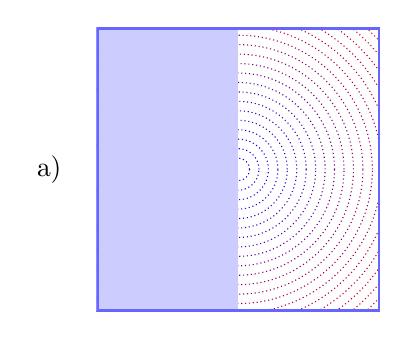
\begin{tikzpicture}[scale=1.2]
            \node[] at (-2, 0) {a)};
            \begin{scope}
                \clip (-1.5, -1.5) rectangle (1.5, 1.5);
                \foreach \cRadius in {1, ..., 22}
                    \pgfmathsetmacro\cColor{\cRadius/22*100}
                    \draw[red!\cColor!blue, densely dotted] (0, 0) circle (0.02+\cRadius*0.1); 
                    
                \fill[blue!20] (-1.5, -1.5) rectangle (0, 1.5);
                \draw[blue!60, ultra thick] (-1.5, -1.5) rectangle (1.5, 1.5);
            \end{scope}
        \end{tikzpicture}
        \qquad
        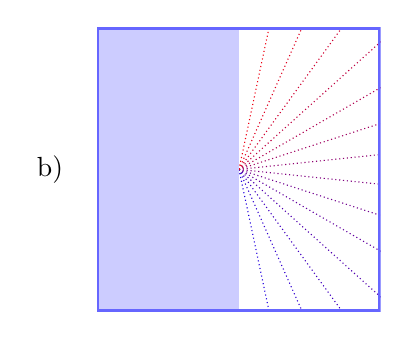
\begin{tikzpicture}[scale=1.2]
            \node[] at (-2, 0) {b)};
            \begin{scope}
                \clip (-1.5, -1.5) rectangle (1.5, 1.5);
                \foreach \cAngle in {1, ..., 16}
                    \pgfmathsetmacro\cColor{\cAngle/16*100}
                    \draw[red!\cColor!blue, densely dotted] (0, 0) -- (\cAngle* 180 / 15 -102:3); 
                \fill[blue!20] (-1.5, -1.5) rectangle (0, 1.5);
                \draw[blue!60, ultra thick] (-1.5, -1.5) rectangle (1.5, 1.5);
            \end{scope}
        \end{tikzpicture}
    \end{center}
    \caption{Schéma représentant l'extraction de caractéristiques à partir de l'espace de Fourier. En a), l'utilisation de cercle concentrique depuis l'origine, schématisé en pointillés; En b), l'extraction selon une direction.}
    \label{fig:scheme_fourier_features}
\end{figure}\par

La transformée en ondelettes possède divers avantages dont une bonne capacité de localisation, par translation de l'ondelette mère, et la possibilité de prendre en considération plusieurs échelles d'analyse, par homothétie~\cite{Livens1997,Wiltgen2008}. Concernant le choix de l'ondelette mère, celui-ci ne semble pas affecter la qualité des caractéristiques extraites~\cite{Fatemi1996, Livens1997}. Néanmoins, l'un des auteurs préconise le choix d'ondelette symétrique ou anti-symétrique~\cite{Livens1997}. Plusieurs de nos références s'orientant vers des ondelettes de Daubechies, nous privilégierons ces dernières~\cite{Wiltgen2008,Halimi2017a}. La décomposition est ainsi réalisée à divers niveaux afin de capter plusieurs niveaux de détail. La décomposition d'un niveau se réalise en 3 étapes successives: 
\begin{inlinerate}
    \item de filtrage passe-bas et passe-haut horizontal,
    \item de filtrage passe-bas et passe-haut vertical,
    \item puis une étape de sous-échantillonage afin de réduire limiter la quantité d'information.
\end{inlinerate} La totalité de ce processus est schématisé en \Cref{fig:scheme_dwt}. Les mesures statistiques extraites préconisés à ces diverse échelles sont la déviation standard, l'énergie et l'entropie~\cite{Livens1997, Wiltgen2008}. La transformée en ondelettes sera effectuée dans le reste de ce travail par la bibliothèque logicielle "PyWavelets"~\cite{lee2006}.\par

\begin{figure}[H]
\centering
    \begin{subfigure}{.45\textwidth}
      \centering
      \includegraphics[width=\textwidth]{contents/chapter_4/resources/scheme_dwt.pdf}
    \end{subfigure}
    \vrule
    \begin{subfigure}{.45\textwidth}
      \centering
      \includegraphics[width=\textwidth]{contents/chapter_4/resources/scheme_dwt_decomposition.pdf}
    \end{subfigure}
    \caption{Principe de la décomposition en ondelettes appliquée aux images~\cite{Livens1997}. A gauche, la décomposition est réalisée en trois temps. Un filtrage passe bas (L) et passe haut (H) sont réalisés selon la direction horizontale, puis selon la direction verticale. Enfin, un sous échantillonage de coefficient 2 est appliqué afin d'obtenir un matrice de même taille que l'image d'origine. A droite, les  deux principaux types de décomposition successives: par schéma pyramidal ou arbre dyadique, et par structure d'arbre.}
    \label{fig:scheme_dwt}
\end{figure}\par

Le premier travail réalisé par Wiltgen~\cite{Wiltgen2008} met à disposition deux méthodes d'extraction de caractéristiques à partir de transformations fréquentielles desquelles sont obtenues diverses statistiques. Dans un premier temps, une de ses méthode se base sur la transformée de Fourier, et extrait \textbf{38 descripteurs} de la magnitude du spectre:
\begin{itemize}
    \item \textbf{22 descripteurs} correspondent à la moyenne calculée sur des rayons répartis de manière équidistante du centre du spectre (\Cref{fig:scheme_fourier_features} - a ),
    \item \textbf{16 descripteurs} correspondent à la moyenne calculée sur des directions à intervalles constantes (\Cref{fig:scheme_fourier_features} - b ).
\end{itemize} Dans un second temps, ce même article propose un approche par ondelettes de Daubechies. La transformée est ainsi calculée à cinq niveau successif sous forme d'arbre diadique, et préconise l'extraction de 3 mesures statistiques (la déviation standard, l'énergie et l'entropie) par bande de fréquences pour un total de \textbf{39 descripteurs}.\par

Le second travail sur lequel nous nous appuyons est une forme d'extension de la transformée en ondelettes du précédent travail~\cite{Halimi2017a}. Cette transformée est réalisée de manière diadique à quatre niveaux différents de décomposition. L'auteur y propose une extraction statistique différente des précédents travaux, reposant sur une approximation à chaque niveau de décomposition par une loi normale généralisée centrée dont la densité de probabilité $f$ est décrite par l'\Cref{eq:ggd}. Les auteurs de l'étude ne retiennent comme caractéristiques que les paramètres d'échelle $\alpha$ et de forme $\beta$.\par
\begin{equation}
    f(x)= \frac{\beta}{2\alpha\Gamma(1/\beta)} e^{-\left(|\frac{x}{\alpha}|\right)^\beta}
    \label{eq:ggd}
\end{equation}
 
Ainsi, nous réaliserons plusieurs expériences sur base de descripteurs manuels en fréquence. Dans un premier temps, nous tenterons d'étudier l'impact des méthodes standards. Puis dans un second temps, nous reproduirons les méthodes de la littérature proche de notre thématique et précédemment détaillés~\cite{Wiltgen2008, Halimi2017a}. La \Cref{tab:number_features_frequency} synthétise le nombre associé de caractéristiques extraites par ces diverses méthodes d'extraction fréquentielles.\par

\begin{table}[h]
    \centering
    \begin{tabular*}{0.6\linewidth}{l@{\extracolsep{\fill}}l}
        \toprule
        \textbf{Méthode}                        & \textbf{Nombre}   \\ \hline
        Fourier                                 & 10/20/30          \\ \hline
        Ondelettes                              & XX                \\ \hline
        Wiltgen~\cite{Wiltgen2008} - Fourier    & 38(22+16)         \\ \hline
        Wiltgen~\cite{Wiltgen2008} - Ondelettes & 39(13$\times$3)   \\ \hline
        Halimi~\cite{Halimi2017a} - Ondelettes  & 24(12$\times$2)   \\
        \bottomrule
    \end{tabular*}
    \caption{Nombre de caractéristiques extraites par méthode spatiale.}
    \label{tab:number_features_frequency}
\end{table}\par

\subsection{Technique d'apprentissage par transfert de connaissances}
Les techniques d'apprentissage par transfert de connaissances sont un champs d'application relativement récent en comparaison des techniques d'apprentissage automatique. Le principe est la réutilisation de connaissances précédemment acquises dans le but de résoudre de nouveau problèmes plus rapidement, voir plus efficacement. Pour cela, ce champs vise à  proposer des moyens d'extraire les connaissances d'une ou plusieurs tâches sources, et de les appliquer à une tâche cible~\cite{QiangYang2010}.\par
Haar ~\cite{Ghazali2007}
Le récent engouement pour les \gls{cnn} et la complexité des architectures actuelle pour le traitement des images à accentué les recherches en ce sens. En effet, les techniques d'apprentissage par transfert de connaissance sont une réponse efficace à de nombreuses problématiques autour de l'entraînement des \gls{cnn}, comme: 
\begin{itemize}
    \item ses \textbf{contraintes de données}: notamment de données annotées, structurées et disponible publiquement,
    \item sa \textbf{complexité}: comprenant l'exécution parfois multiple de l'entraînement si celui-ci ne converge pas mais également le réglage de certains paramètres de ces réseaux,
    \item et ses \textbf{contraintes matérielles}: la puissance nécessaire à l'entraînement de tels réseaux.
\end{itemize}\par

Certains domaines d'application ont vu apparaître de nombreuses base de données publique, contribuant à résoudre partiellement la contrainte liée aux données. C'est le cas de différentes bases dont: 
\begin{inlinerate}
    \item MNIST pour la reconnaissance chiffres~\cite{lecun2010},
    \item CIFAR10/CIFAR100 pour la reconnaissance d'objets sur des miniatures~\cite{Krizhevsky}, 
    \item ou plus récemment ImageNet pour la reconnaissance d'objets sur des images~\cite{Deng2008}. 
\end{inlinerate}
La base ImageNet est par ailleurs l'une des plus sollicités pour entraîner et évaluer les architecture de \gls{cnn} actuelles, car elle propose de nombreuses images de qualité suffisante (plus de 14 millions d'images sont dénombrées) et des annotations variées (1000 classes différentes sont proposées). Néanmoins, selon certaines études le nombre d'images nécessaires à l'entraînement de ces réseaux serait sur-dimensionné~\cite{huh2016}. Parallèlement à la mise à disposition de ces bases de données, sont également ouvert publiquement des challenges visant à démontrer l'efficacité de chaînes de traitement pour gérer ces dites données. De nombreuses avancées sont proposées et réalisées sur la base ImageNet à d'architecture de \gls{cnn}, également mise à disposition de la communauté. Parmi ces réseaux nous pouvons citer de manière exhaustive: AlexNet~\cite{Krizhevsky2012}, GoogLeNet~\cite{Szegedy2015}, VGG-16~\cite{Simonyan2014}, Inception-V3~\cite{Szegedy2016}, ResNet~\cite{He2016} et Inception-ResNet~\cite{Szegedy2017}, avec respectivement comme précisions 0.54, 0.68, 0.71, 0.76, 0.78, and 0.80 sur la base ImageNet~\cite{Canziani2016}.\par

Néanmoins, la mise à disposition de la communauté de base de données massives, et de codes permettant de reproduire les expériences menées sur la plupart des architectures actuelles ne permettent pas de répondre à la problématique des contraintes matérielles. C'est donc particulièrement le partage de modèles de \gls{cnn} pré-entraînés, couplé aux principes d'apprentissage par transfert de connaissances qui ont suscité l'intérêt de nombreux papiers de recherche, notamment appliqué à de l'imagerie médicale~\cite{Litjens2017}. La grandes majorité des modèles mis à disposition par la communauté sont le résultat d'un entraînement à partir de la base ImageNet.\par
 
\begin{figure}[H]
    \centering
    \includegraphics[width=\linewidth]{contents/chapter_4/resources/scheme_transfer_learning.pdf}
    \caption{Schéma représentant l'apprentissage par transfert par \gls{cnn}. Le réseau est entraîné sur des données sources, généralement plus complètes. Puis, les paramètres de la partie liée à l'extraction de caractéristiques sont conservés et réemployé au sein d'une nouvelle problématique cible.}
    \label{fig:scheme_transfer_learning}
\end{figure}\par

Au sein de cette partie, nous nous focaliserons sur l'un des deux principes d'apprentissage par transfert de connaissances à savoir l'extraction de caractéristiques, schématisé en \Cref{fig:scheme_transfer_learning}. Le principe consiste à retirer les couches responsable de la classification, et à ne conserver que les couches responsable de l'extraction de l'information caractéristique. Ces couches sont ensuite figées, et combinées à de nouvelles couches ou à des modèles de classification~\cite{Litjens2017}.\par 

Afin de traiter cette information, il sera généralement acquis de transiter l'information par une étape de "Flatten" (littéralement "Applatissement") transformant l'information d'un format  de matrice 3D à un vecteur 1D (voir \Cref{fig:scheme_global_pooling}). Néanmoins, l'une des problématique importante concerne la dimension importante de ces caractéristiques extraites, souvent dépendante sur les derniers réseaux de la taille des données sources. En effet, la sortie sera souvent dépendante de la résolution spatiale des données d'entrée, réduite entre autre par les différentes couches convolutionnelles dont les caractéristiques varient d'une architecture considérée à une autre (soit une résolution de 1000$\times$1000 sur nos données). Pour palier à ce nombre de données, des couches dites de "global pooling" ont été introduite dans la littérature consistant à réduire l'information spatiale d'une carte d'activation à une unique valeur (voir \Cref{fig:scheme_global_pooling}). Les principales fonctions mises à disposition sont la fonction maximum et moyenne, donnant respectivement lieu à des couches de "Global Maximum Pooling" et "Global Average Pooling". D'autres fonction sont également développée, mais la littérature s'accordera à favoriser légèrement les couches de "Global Maximum Pooling"~\cite{christlein2019}.\par

\begin{figure}[H]
    \centering
    \includegraphics[width=\linewidth]{contents/chapter_4/resources/scheme_global_pooling.pdf}
    \caption{Schéma représentant l'aplatissement et la réduction d'information par "Global Pooling" au sein de \gls{cnn}. Le réseau est entraîné sur des données sources, généralement plus complètes. Puis, les paramètres de la partie liée à l'extraction de caractéristiques sont conservés et réemployé au sein d'une nouvelle problématique cible.}
    \label{fig:scheme_global_pooling}
\end{figure}\par

Bien que la plupart des travaux médicaux s'oriente vers l'architecture Inception-V3, aucune raison n'a démontré l'efficacité de cette architecture particulière au sein d'applications médicales. L'une des hypothèses majeure étant la disponibilité de l'architecture et de modèle pré entraînés aisément mis à disposition par la plupart des librairies de \gls{cnn}~\cite{Litjens2017}. Les différentes expériences que nous mènerons sur l'apprentissage par transfert se focaliserons sur des architectures relativement récente pré entraîné sur la base d'image ImageNet et proposé par la bibliothèque "Keras Applications"~\cite{chollet2015a}. Afin de traiter les images dans leur intégralité, nous ne nous baserons que sur des réseaux dont les couches d'extraction de caractéristiques sont purement convolutionnelles et donc indépendante de la taille de l'entrée. Ainsi, nous ne conserverons que quatre d'entre elles: VGG-16, Inception-V3, ResNet et Inception-ResNet. L'ensemble des réseaux employés et nombre de paramètres extraits associés sont résumés au sein de la \Cref{tab:number_features_transferlearning}. Finalement, la manipulation des \ac{cnn} est réalisée à haut niveau grâce à la bibliothèque logicielle "Keras"~\cite{chollet2015} et sera couplée à la bibliothèque de bas niveau "Tensorflow"~\cite{tensorflow2015}.\par

\begin{table}[H]
    \centering
    \begin{tabular*}{0.6\linewidth}{l@{\extracolsep{\fill}}l}
    \toprule
    \textbf{Architecture}        & \textbf{Nombre}          \\ \hline
    VGG-16                       & 512                      \\ \hline
    Inception-V3                 & 2048                     \\ \hline
    ResNet                       & 2048                     \\ \hline 
    Inception-ResNet             & 1536                     \\
    \bottomrule
    \end{tabular*}
    \caption{Nombre de caractéristiques extraites par type d'architecture de \gls{cnn}.}
    \label{tab:number_features_transferlearning}
\end{table}\par
 
\subsection{Analyse préliminaire des méthodes d'extraction}
\begin{figure}[H]
    \centering
    \includegraphics[width=\linewidth]{contents/chapter_4/resources/example_glcm.pdf}
    \caption{Exemple d'extraction de \gls{glcm} de second ordre sur deux images typique. En haut, un cas d'image bénigne; En bas, une image pathologique typique de \gls{lm}.}
    \label{fig:example_glcm}
\end{figure}\par

\begin{figure}[H]
    \centering
    \includegraphics[width=\linewidth]{contents/chapter_4/resources/example_fft.pdf}
    \caption{Exemple de transformée de Fourier appliquée à deux images typiques, représentation selon le module et la phase. En haut, un cas d'image bénigne; En bas, une image pathologique typique de \gls{lm}.}
    \label{fig:example_fft}
\end{figure}\par

\begin{figure}[H]
    \centering
    \includegraphics[width=\linewidth]{contents/chapter_4/resources/example_wavelet.pdf}
    \caption{Exemple de transformée en ondelettes (Daubechies) appliquée à deux images typiques, à 2, 3 puis 4 niveaux. En haut, un cas d'image bénigne; En bas, une image pathologique typique de \gls{lm}.}
    \label{fig:example_wavelet}
\end{figure}\par

\begin{figure}[H]
    \centering
    \begin{subfigure}{.5\textwidth}
      \includegraphics[width=\textwidth]{contents/chapter_4/resources/visualisation_spatial_first.png}
    \end{subfigure}
    
    \begin{subfigure}{.45\textwidth}
      \includegraphics[width=\textwidth]{contents/chapter_4/resources/visualisation_spatial_haralick.png}
    \end{subfigure}
    \begin{subfigure}{.45\textwidth}
      \includegraphics[width=\textwidth]{contents/chapter_4/resources/visualisation_spatial_haralickmean.png}
    \end{subfigure}
    
    \begin{subfigure}{.45\textwidth}
      \includegraphics[width=\textwidth]{contents/chapter_4/resources/visualisation_spatial_Wiltgen.png}
    \end{subfigure}
    \begin{subfigure}{.45\textwidth}
      \includegraphics[width=\textwidth]{contents/chapter_4/resources/visualisation_spatial_WiltgenAll.png}
    \end{subfigure}
    
    \caption{Visualisation des caractéristiques obtenues par techniques d'extraction spatiales et projection \gls{pca} sur les deux premières composantes.}
    \label{fig:visualisation_spatial}
\end{figure}\par

\begin{figure}[H]
    \centering
    \begin{subfigure}{.45\textwidth}
      \includegraphics[width=\textwidth]{contents/chapter_4/resources/visualisation_frequency_Fourier10.png}
    \end{subfigure}
    \begin{subfigure}{.45\textwidth}
      \includegraphics[width=\textwidth]{contents/chapter_4/resources/visualisation_frequency_Fourier20.png}
    \end{subfigure}
    
    \begin{subfigure}{.45\textwidth}
      \includegraphics[width=\textwidth]{contents/chapter_4/resources/visualisation_frequency_Fourier30.png}
    \end{subfigure}
    \begin{subfigure}{.45\textwidth}
      \includegraphics[width=\textwidth]{contents/chapter_4/resources/visualisation_frequency_wiltgenfourier.png}
    \end{subfigure}
    
    \begin{subfigure}{.3\textwidth}
      \includegraphics[width=\textwidth]{contents/chapter_4/resources/visualisation_frequency_dwthaar.png}
    \end{subfigure}
    \begin{subfigure}{.3\textwidth}
      \includegraphics[width=\textwidth]{contents/chapter_4/resources/visualisation_frequency_wiltgendwt.png}
    \end{subfigure}
    \begin{subfigure}{.3\textwidth}
      \includegraphics[width=\textwidth]{contents/chapter_4/resources/visualisation_frequency_halimidwt.png}
    \end{subfigure}
    
    \caption{Visualisation des caractéristiques obtenues par techniques d'extraction fréquentielles et projection \gls{pca} sur les deux premières composantes.}
    \label{fig:visualisation_frequency}
\end{figure}\par

\begin{figure}[H]
    \centering
    \begin{subfigure}{.2\textwidth}
      \includegraphics[width=\textwidth]{contents/chapter_4/resources/visualisation_transfer_vgg16avg.png}
    \end{subfigure}
    \begin{subfigure}{.2\textwidth}
      \includegraphics[width=\textwidth]{contents/chapter_4/resources/visualisation_transfer_inceptionv3avg.png}
    \end{subfigure}
    \begin{subfigure}{.2\textwidth}
      \includegraphics[width=\textwidth]{contents/chapter_4/resources/visualisation_transfer_resnetavg.png}
    \end{subfigure}
    \begin{subfigure}{.2\textwidth}
      \includegraphics[width=\textwidth]{contents/chapter_4/resources/visualisation_transfer_inceptionresnetv2avg.png}
    \end{subfigure}
    
    \begin{subfigure}{.2\textwidth}
      \includegraphics[width=\textwidth]{contents/chapter_4/resources/visualisation_transfer_vgg16max.png}
    \end{subfigure}
    \begin{subfigure}{.2\textwidth}
      \includegraphics[width=\textwidth]{contents/chapter_4/resources/visualisation_transfer_inceptionv3max.png}
    \end{subfigure}
    \begin{subfigure}{.2\textwidth}
      \includegraphics[width=\textwidth]{contents/chapter_4/resources/visualisation_transfer_resnetmax.png}
    \end{subfigure}
    \begin{subfigure}{.2\textwidth}
      \includegraphics[width=\textwidth]{contents/chapter_4/resources/visualisation_transfer_inceptionresnetv2max.png}
    \end{subfigure}
    
    \caption{Visualisation des caractéristiques obtenues par techniques d'extraction basé sur des réseaux de type \gls{cnn} pré-entraînés sur la base ImageNet et projection \gls{pca} sur les deux premières composantes.}
    \label{fig:visualisation_transfer}
\end{figure}\par

%%%%%%%%%%%%%%%%%%%%%%%%%%%%%%%%%% 
%%%%%%%%%%%%%%%%% PRE TRAITEMENTS
\section{Pré-traitements de caractéristiques}
Cette partie dédié au pré-traitement de caractéristique se consacre à l'ensemble des transformations opérées après extraction de l'information par le biais des techniques évoquées en \Cref{chap:feature_extraction}. Nous aborderons au sein de cette section les diverses solutions à notre disposition pouvant parfaire la classification de notre problématique. En effet, de nombreuse contraintes peuvent affecter le bon déroulement de la classification:
\begin{enumerate}
    \item un déséquilibre des annotations (essentiellement dans les situations à deux classes -  tissus pathologique et non pathologiques; tissus malin et tissus autres),
    \item une quantité d'informations trop importante conduisant à un sur apprentissage, situation que nous rencontrons avec l'extraction de caractéristiques par \gls{cnn},
    \item ou encore une information inconsistante.
\end{enumerate}\par

Ainsi, cette partie tentera de répondre à ces questions à l'aide de différents domaines d'étude visant à corriger tout ou partie de ces éléments. Dans un premier temps, nous discuterons de la \textbf{normalisation} et son intérêt au sein de processus de classification. Dans un second temps, nous aborderons le \textbf{balancement de données} et les principales stratégies mises à disposition. Finalement, nous traiterons des techniques de \textbf{réduction de l'information} et proposerons des solutions notamment dans le cadre de l'extraction de caractéristiques par \gls{cnn}.

\subsection{Normalisation de caractéristiques}
Selon le domaine visée, la normalisation de caractéristiques peux-être l'une des étapes cruciale quand au bon déroulement du processus de classification. Un exemple proche de nos travaux, sur la classification d'image de dermatoscopie, menée par Celebi et al., est un parfait exemple de la dégradation des résultats de classification avec l'utilisation de caractéristiques brutes ~\cite{Celebi2007}. Notre investigation de la littérature à également mis en évidence que des algorithmes de classification tel que la méthode des \textbf{k plus proches voisins} sont affectés car directement basé sur un critère de distance. D'autres modèles sont communément admis comme touchés par des caractéristiques non normalisées: les \gls{svm}~\cite{Juszczak2002}, mais également les réseaux de neurones~\cite{Celebi2007} en sont de très bon exemples. De même, des méthodes de réduction de l'information, que nous traiterons lors des prochaines, peuvent être affectées par une mauvaise distribution de l'information. Par exemple, le \gls{pca} est une méthode dont l'algorithme tente de maximiser la variance pouvant être impactée négativement (voir \Cref{fig:exemple_pca_scaling}).\par

\begin{figure}[H]
    \centering
    \includegraphics[width=0.8\linewidth]{contents/chapter_4/resources/example_pca_scaling.pdf}
    \caption{Exemple de l'impact de la distribution de données sur le \gls{pca} appliqué à une analyse chimique du vin en provenance de différentes région~\textsuperscript{\ref{footnote:exemple_pca_scaling}}. A gauche, le résultat issu du \gls{pca} sans normalisation préalable; A droite, la distribution après normalisation et \gls{pca}.}
    \label{fig:exemple_pca_scaling}
\end{figure}\par

\addtocounter{footnote}{1}
\footnotetext[\thefootnote]{Source : Scikit-learn - \href{https://scikit-learn.org/stable/auto_examples/preprocessing/plot_scaling_importance.html}{"Importance of Feature Scaling"}. \label{footnote:exemple_pca_scaling}}

Divers travaux ont ainsi été menés, afin de proposer des méthodes de normalisation à cette problématique. L'un de ces travaux propose trois méthodes de normalisation par la variance, par le maximum, et par le minimum et maximum dans le contexte de \gls{svm}~\cite{Juszczak2002}. Ces trois méthode semblent ainsi propice à réduire l'erreur de classification. Le travail mené par Celebi et al.~\cite{Celebi2007}, propose une normalisation des caractéristiques à l'aide de la "Cote Z" ou "Standard score", c'est à dire par soustraction de la moyenne au sein d'un même groupe de caractéristiques puis par division de l'écart type de ce même groupe.\par

Afin de couvrir au mieux la problématique de la normalisation, nous traiterons cette problématique sous trois méthodes majeures:
\begin{itemize}
    \item l'utilisation de la normalisation "Min-Max"~\cite{Juszczak2002},
    \item l'utilisation de la normalisation "Standard"~\cite{Celebi2007}, 
    \item et l'utilisation de la normalisation "Robust". 
\end{itemize}
Ces diverses méthode de normalisation seront évalué face à un processus n'employant aucune d'entre elles, nous servant ainsi de méthode de comparaison. De plus ces méthodes seront réalisées en amont du processus de pré traitement afin de couvrir également les méthodes de réduction de l'information pouvant être affectées. L'\Cref{eq:scaling_methods} couvre les diverses équations listé précédemment.\par

\begin{equation} 
    \label{eq:scaling_methods}
    \begin{split}
    &MinMax=\frac{X-min(X)}{max(X)-min(X)}  \\
    &Standard=\frac{X-\mu{}}{\sigma}	    \\
    &Robust=\frac{xi–Q1(x)}{Q3(x)–Q1(x)}    \\
    \end{split}
\end{equation}

\subsection{Balancement de caractéristiques}
L'une des problématiques associés de manière récurrente aux problématiques d'apprentissage sur des données réelles, en opposition avec des données provenant de modèle génératifs par exemple, est celle de la répartition homogène des annotations. Ces déséquilibres pouvant survenir au sein des annotations sont qualifié sous le terme anglais de "class imbalancement"~\cite{Prati2009, He2009}.\par

Cette problématique est récurrente à de nombreux domaines d'applications, mais touche essentiellement les domaines où la tâche visée correspond à la détection d'événements isolés au sein d'une population, comme par exemple: 
\begin{inlinerate}
    \item les comportements déviants (fraude bancaire~\cite{Phua2004}),
    \item le respect de critère de qualité (vérification de pièces industrielles~\cite{Wu2018}),
    \item ou encore dans notre domaine d'anormalités clinique (cancers ou d'autres pathologies cliniques~\cite{Celebi2007}),
    \item \ldots
\end{inlinerate}\par

Certains choix peuvent permettre de limiter l'impact d'un déséquilibre d'annotations. Ainsi, la sélection d'un métrique adéquate peux permettre de limiter la dépendance au données: la substitution de la précision par des mesures telles que l'\gls{auc}~\cite{Celebi2007} ou le f1-score sont des solutions pertinentes dans de telles situations. Néanmoins, la plupart des modèles de classification échouerons à classifier convenablement les données dans des situations de fort déséquilibres. Ces modèles préférerons prédire constamment la classe majoritaire, pour minimiser le coût de l'erreur~\cite{Huang2013}. Dans le cadre de modèles basés sur des arbres de décision, la stratégie générale propose de déterminer les critères majeurs de séparation par partitionnement successif des données. Ce partitionnement conduit inéluctablement à un affaiblissement des classes minoritaires~\cite{He2009}.\par 

Afin de corriger ces éléments, deux catégories d'approches ont été proposées pour solutionner ce déséquilibre~\cite{Huang2013}. Les approches par corrections de donnée procède par augmentation ou décimations de ces dernières afin de rééquilibré les annotations. Les approches algorithmiques consistent à pondérer la valeur des annotations afin de prendre en considération le déséquilibre d'information~\cite{Ting2002,He2009,Thai2010}.\par

En premier lieu, des approches par correction des données simples, proposes diverses solutions pour palier à ces déséquilibres de classes~\cite{Prati2009, He2009}. Une première catégories de ces méthodes consiste à \textbf{sous-échantillonner} les données jusqu'à obtenir une égalité entre les classes. Son principe le plus simple est celui du "Sous-échantillonage aléatoire" consistant à décimer de manière aléatoire les données des classes majoritaire afin d'égaler les échantillons de la classe minoritaire. A l'inverse, une autre catégorie consiste à \textbf{sur-échantillonner} les données possédées afin d'obtenir à nouveau une égalité entre classes. Le principe le plus simples est celui du "Sur-échantillonage aléatoire" consistant à dupliquer aléatoirement les échantillons des classes minoritaires afin d'égaler le nombre d'élément de la classe majoritaire. Le schéma en \Cref{fig:scheme_data_balancing} reprendre l'idée de ces deux principes.\par

\begin{figure}[H]
    \centering
    \includegraphics[width=\linewidth]{contents/chapter_4/resources/scheme_data_balancing.pdf}
    \caption{Schéma des deux stratégies principales de balancement de données. A gauche, la stratégie de sous-échantillonage, dans laquelle des éléments sont aléatoirement choisis jusqu'à réduire l'ensemble des classes au nombre d'éléments de la classe minoritaire; A droite, la stratégie de sur-échantillonage, dans laquelle les éléments des classes minoritaires sont dupliqués aléatoirement. }
    \label{fig:scheme_data_balancing}
\end{figure}\par

En second lieu, des approches par correction des données plus avancées ont été proposées. De manière non exhaustive nous proposerons l'une d'entre elle pour chaque catégories:
\begin{itemize}
    \item par \textbf{sous-échantillonnage}: \cite{Tomek1976}
    \item par \textbf{sur-échantillonnage}:\cite{Chawla2002} 
    \item par \textbf{combinaison}: SMOTE + Tomek
    \item \ldots
\end{itemize}\par

Les approches algorithmique par pondération, consiste à considérer le non balancement de l'information en pondérant l'importance de chaque échantillon lors de l'apprentissage du modèle.  

Dans l'optique de récapituler cette partie, les méthodes utilisées dans le but de corriger le déséquilibre des données sont référencée dans la \Cref{tab:summary_balancement_methods}. Afin de traiter au mieux cette tâche, la balancement de données par ses différentes stratégies évoquée sera réalisé avec l'aide de la librairie logicielle "Imbalanced-learn"~\cite{Lemaitre2017}. La correction par algorithme, plus précisément pondération, sera réalisé avec l'aide de la bibliothèque "Scikit-learn"~\cite{pedregosa2011}.\par

\begin{table}[H]
    \centering
    \begin{tabular*}{0.6\linewidth}{l@{\extracolsep{\fill}}l}
    \toprule
    \textbf{Catégorie}                  & \textbf{Méthode}                  \\ \hline
    \multirow{2}{*}{Sous-échantillonage}& Sous-échantillonage aléatoire     \\ \cline{2-2}
                                        & Tomek Link                        \\ \hline
    \multirow{2}{*}{Sur-échantillonage} & Sur-échantillonage aléatoire      \\ \cline{2-2}
                                        & SMOTE                             \\ \hline
    Combinaison                         & SMOTE + Tomek                     \\ \hline 
    Algorithme                          & Pondération                       \\
    \bottomrule
    \end{tabular*}
    \caption{Liste des diverses méthodes de balancement mises en oeuvre pour corriger les déséquilibre de données.}
    \label{tab:summary_balancement_methods}
\end{table}\par

\subsection{Réduction de dimensions}
Dans le domaine de l'apprentissage automatique, la réduction de dimension est une technique qui permet de réduire l'information extraites afin de rendre un problème moins complexe. Également, elle est un moyen de se prévenir du "Fléau de la dimension", phénomène qui met en perspective d'une part la croissance exponentielle de l'ajout de nouvelles dimensions à la dilution des divers échantillons dans cet espace. Ce dilemme a pour principales conséquences d'augmenter la complexité d'un problème, la durée nécessaire à sa résolution mais également d'engendrer des risques de sur-apprentissage.\par

A cette fin, deux catégories de méthodes cohabitent: d'une part les méthode de sélection de caractéristiques, qui réduise l'espace en décimant certaine dimension jugées non pertinente à la résolution du problème; d'autre part les méthode par projection ou transformation de l'espace existant qui réduisent et modifie les valeurs existantes. Notre investigation ne portera que sur cette seconde catégorie de méthodes.\par

pca\par
lda\par~\cite{Nanni2017}


\section{Méthodes de prédiction}

\section{Processus et metriques}
\section{Résultats}


Néanmoins, il est également a été également jugées important de l'intersection d'évènements tels que la présence de tissus caractéristiques aux abords de follicules pileux.\par
\chapter{Amélioration du diagnostic image}
\label{chap:chapter_5}
\todo[inline,color=red, caption={}]{
    \begin{itemize}  
        \item multi patch
        \item multi resolution
    \end{itemize}
}
%=====================================
% PATIENT LEVEL
%=====================================
\chapter{Prise de décision patient}
\label{chap:chapter_6}
\chapterintro
Comme 	
\newpage

\section{Calibration de modèles}
\section{Fusion de décisions}
% Mil & Majority vote\cite{Sudharshan2019}
\section{Approche faiblement supervisée}
\begin{figure}[H]
    \centering
    \includegraphics[width=\linewidth]{contents/chapter_6/resources/scheme_patient_decision.pdf}
    \caption{Schéma de représentation du système complet pour la prise de décision patient supervisée.}
    \label{fig:scheme_patient_decision}
\end{figure}\par
\section{Résultat patient}
% This part relates to different ways to achieve classification at the patient-level based on the same two categories: “malignant”, as the positive class, and “benign”. With this assumption, a patient should be considered “malignant” if at least one image is considered to be “malignant”. Additionally, this part needs to consider the varying number of samples per patient (as a reminder, the number of instances per patient can vary between 2 and 833 images).\par
% In order to achieve this, the best combination of the feature extraction method and the classification model from \Cref{sec:image_decision} was used. The classification model provided two types of information for each image: the score was based on prediction probabilities and the decision (i.e., the class that achieved the best probability). In both cases, due to the varying number of images per patient, the information needs to be transformed into constant-size matrices to make a decision for existing and for new patients. At the score level, the structure was composed of patients, images, and scores of classes and transformed into a new matrix of size P*C, where P is the number of patients and C is the number of classes. A dynamic threshold was then used to adjust the positive class that maximizes the chosen metric. Multiple strategies can be used to achieve this:
% \begin{itemize}
% \item Mean - allows the contribution of each instance on the patient to be retained
% \item Maximum – retention of the best confidence prediction as to the trusted one.
% \end{itemize}
% \begin{figure}[H]
%     \begin{center}
%         \includegraphics[width=0.8\linewidth]{Figures/Process_Decision.pdf}
%         \caption{The classification process performed on \ac{rcm} patients in which the first part of the process remained the same as in \Cref{sec:image_decision}. The “Fit Model” and “Prediction” boxes refer to the decision and score level methods discussed in \Cref{sec:patient_decision}. The testing set was predicted for the patients based on “benign” and “malignant” classes.}
%         \label{fig:decision_process}
%     \end{center} 
% \end{figure}\par
% At the decision level, the structure was composed of structure, combining patients, images, and scores of classes and transformed into a new matrix of size P*C, where P is the number of patients and C is the number of classes. Also, C refers to the probability vector of each decision between 0 and 1.
% \begin{itemize}
% \item At Least One - at least one positive decision to consider the input as positive (initial assumption)
% \item Dynamic - find a dynamic threshold that minimizes false-positive decisions.
% \end{itemize}
% A global overview of the processing scheme of this method is presented in \Cref{fig:decision_process}.
% In a second stage, a number of \ac{mil} concepts are implemented in this part, as they fit the issue at hand: a patient is constitutive of several instances (consider it as a bag) and a positive instance assumes that the patient should be positive. Furthermore, only the patient label is known, and the annotation step of individual images is time-consuming. Such a problem can be set as a pair\(\{X|y\}\), in which \(X=\{X^1,X^2,\ldots,X^b\}\) is a bag containing \(b\) instances and each \(X^b\) formulated as follows: \(X^b=\{x^b_1,x^b_2,\ldots,x^b_n\}\), in which \(n\) is the number of features and \(y\) is the patient label~\cite{foulds_frank_2010}. Two ideas are developed regarding this context in the paragraphs that follow. In a first stage, a \ac{sil} classification is used in which a bag is considered as negative if all of the instances are considered to be negative, and positive if at least one of the instances has a positive label that fits our initial formulation of the patient label. In a second stage, the MI-SVM is an extension of \ac{svm} upon \ac{mil} theory and is employed in these due to the results of \Cref{sec:image_decision}. These experiments are configured to function with a linear kernel due to the observation made by the experiments of \Cref{sec:image_decision}. In this part, the experiments were implemented using the “MISVM” library~\cite{Doran2014}.\par
% In addition, to provide the best performance on each of these models, a search for their optimal hyper-parameters was carried out (see \Cref{tab:patient_hyperparameters}).\par
% \begin{table}[H]
%     \centering
%     \begin{tabular}{llll}
%     \textbf{Category}               & \textbf{Name}     & \textbf{Parameter}& \textbf{Values}                                   \\ \hline
%     \multirow{2}{*}{Score}          & Mean              & \multirow{2}{*}{-}& \multirow{2}{*}{[]}                               \\ \cline{2-2}
%                                     & Maximum           &                   &                                                   \\ \hline 
%     \multirow{2}{*}{Decision}       & At Least One      & \multirow{2}{*}{-}& \multirow{2}{*}{[]}                               \\ \cline{2-2}
%                                     & Dynamic           &                   &                                                   \\ \hline 
%     \multirow{2}{*}{\ac{mil}}       & \ac{sil}          & \multirow{2}{*}{C}& \multirow{2}{*}{[0.01, 0.1, 1, 10, 100, 1000]}    \\ \cline{2-2}
%                                     & MI-SVM            &                   &                                                   \\ \hline 
%     \end{tabular}    
%     \caption{List of all of the classification models and referring evaluated hyper-parameters.}
%     \label{tab:patient_hyperparameters}
% \end{table}\par

% The validation protocol remains the same for each of these experiments, based on a nested cross-validation that is known to be less biased than a simple cross-validation scheme~\cite{Cawley2010}. This protocol allows 1) cross-validation of hyper-parameters and 2) objective evaluation of the prediction models. Each of the cross-validation step is based on a K-fold strategy with a $k$ value of 4 on the testing loop and 2 on the validation loop. Also, each time, the patients are separated and balanced as best as possible based on the image labels. In order to achieve an objective evaluation, each data cluster remains the same for the experiments in a given section (refer to \Cref{sec:image_decision} and \Cref{sec:patient_decision}). Moreover, each experiment is validated and evaluated using a \fscore{} metric, as it is statistically suitable for unbalanced populations in comparison with accuracy, and it represents in a single value both recall and precision information. In addition, standard deviation is computed to analyse the stability of models along the nested cross-validation. For this purpose, we used the “Scikit Learn” library for Machine Learning classification, validation, and metric~\cite{pedregosa2011scikit}.\par


% This paragraph focuses on the methods implemented to reach the patient diagnosis (see \Cref{sec:patient_decision}) and it relates to the initial \ac{rcm} data (including unlabeled images) used previously to evaluate specialists~\cite{Cinotti2018}. All these experimental results are listed in \Cref{tab:patient_results} and discussed below. Firstly, the methods performance varied between 0.61 and 0.84 in terms of the \fscore{} for Malignancy. The “At Least One” method achieved poor performance due to prediction errors over the “benign” class. This problem can be solved by the use of a dynamic activation threshold for decisions to minimize the risk of false-positives, at the cost of resulting in an ethical consideration of this method in the clinical context. Secondly, the methods based on the score are almost the same and varied from 0.76 to 0.83 for the \fscore{} for Malignancy. By contrast, with these results, the standard deviations remained reasonable, varying from 0.03 to 0.06. Finally, \ac{mil} was also evaluated, and a substantial difference was noted between the \ac{sil} and the MI-SVM. Indeed, the \ac{sil} assumption yielded similar results with the decision based on the “At Least One” method, due to an insufficient ability to discriminate on the same “benign” class. By contrast, the MI-SVM yielded a number of good results, with an \fscore{} of 0.82. Both methods are stable, with a deviation that only varied from 0.02 to 0.04. Poor results with the “At Least One” and the \ac{sil} methods can be due to a lack of discriminative information provided by the “Inception-ResNet” for these methods.\par
% \begin{table}[H]
%     \centering
%     \begin{tabular}{lllll}
%                                 &                   & \multicolumn{3}{c}{\textbf{Malignancy - \fscore{}}}                    \\ \hline
%     \textbf{Category}           & \textbf{Name}     & \textbf{Weighted}     & \textbf{Benign}       & \textbf{Malignant}    \\ \hline
%     \multirow{2}{*}{Decision}   & At Least One      & 0.61$\pm$0.06         & 0.32$\pm$0.07         & 0.79$\pm$0.05         \\ \cline{2-5} 
%                                 & \textbf{Dynamic}  & \textbf{0.84$\pm$0.03}& \textbf{0.78$\pm$0.07}& \textbf{0.87$\pm$0.02}\\ \hline 
%     \multirow{2}{*}{Score}      & Mean              & 0.83$\pm$0.03         & 0.78$\pm$0.08         & 0.87$\pm$0.02         \\ \cline{2-5}
%                                 & Maximum           & 0.76$\pm$0.04         & 0.68$\pm$0.03         & 0.80$\pm$0.05         \\ \hline  
%     \multirow{2}{*}{\ac{mil}}   & \ac{sil}          & 0.70$\pm$0.04         & 0.50$\pm$0.10         & 0.83$\pm$0.03         \\ \cline{2-5} 
%                                 & \textbf{MI-SVM}   & \textbf{0.82$\pm$0.02}& \textbf{0.78$\pm$0.05}& \textbf{0.84$\pm$0.02}\\ \hline 
%     \end{tabular}    
%     \caption{Results for the patient-level classification for Malignancy (\ac{lm} and \ac{bcc}) according to the different methods from \Cref{sec:patient_decision}. For Malignancy and \ac{lm}, the table provides a weighted average \fscore{} and individual \fscore{} for the benign and the malignant classes.}
%     \label{tab:patient_results}
% \end{table}\par
% Following previous results, this paragraph discusses in detail the results of supervised “Dynamic” decision threshold and \ac{mil} based on “MI-SVM” methods over the Malignancy (meaning \ac{bcc} and \ac{lm}) and \ac{lm} as the cited clinical study does~\cite{Cinotti2018}. \Cref{tab:patient_results_details} provides \fscore{}, precision, and recall based on these experiments. As the classification is binary, recall of the positive class refers to the sensitivity and recall of the negative class refers to the Specificity. The “Dynamic” method achieves scores of 0.89$\pm$0.03 sensitivity and 0.75$\pm$0.07 specificity for Malignancy; 0.88$\pm$0.04 sensitivity and 0.75$\pm$0.07 specificity for \ac{lm} pathologies. The “MI-SVM” method achieves scores of 0.80$\pm$0.02 sensitivity and 0.84$\pm$0.05 specificity for Malignancy; 0.78$\pm$0.07 sensitivity and 0.84$\pm$0.07 specificity for \ac{lm} pathologies. The “Dynamic” method provides more emphasis on sensitivity while “MI-SVM” provides a good specificity. These methods are quite comparable to the evaluation of the dermatologists, reaching 0.80 of sensitivity and 0.81 of specificity, but less homogeneous compared to them.\par
% \par
% \begin{table}[H]
%     \centering
%     \begin{tabular}{lllll||lll}
%                                 &                   & \multicolumn{3}{c}{\textbf{Malignancy}}                               & \multicolumn{3}{c}{\textbf{\ac{lm}}}                                  \\ \hline
%     \textbf{Name}               & \textbf{Label}    & \textbf{\fscore{}}     & \textbf{Precision}    & \textbf{Recall}       & \textbf{\fscore{}}     & \textbf{Precision}    & \textbf{Recall}       \\ \hline
%     \multirow{3}{*}{Dynamic}    & Benign            & 0.78$\pm$0.07         & 0.81$\pm$0.08         & 0.75$\pm$0.07         & 0.79$\pm$0.06         & 0.82$\pm$0.07         & 0.75$\pm$0.07         \\ \cline{2-8}  
%                                 & Malignant         & 0.87$\pm$0.02         & 0.85$\pm$0.03         & 0.89$\pm$0.03         & 0.86$\pm$0.03         & 0.83$\pm$0.03         & 0.88$\pm$0.04         \\ \cline{2-8} 
%                                 & Weighted          & 0.84$\pm$0.03         & 0.84$\pm$0.03         & 0.84$\pm$0.03         & 0.83$\pm$0.03         & 0.83$\pm$0.03         & 0.83$\pm$0.03         \\ \hline
%     \multirow{3}{*}{MI-SVM}     & Benign            & 0.78$\pm$0.02         & 0.72$\pm$0.08         & 0.84$\pm$0.07         & 0.78$\pm$0.05         & 0.73$\pm$0.07         & 0.84$\pm$0.07         \\ \cline{2-8}
%                                 & Malignant         & 0.84$\pm$0.02         & 0.89$\pm$0.05         & 0.80$\pm$0.05         & 0.82$\pm$0.03         & 0.87$\pm$0.06         & 0.78$\pm$0.07         \\ \cline{2-8} 
%                                 & Weighted          & 0.82$\pm$0.02         & 0.82$\pm$0.02         & 0.83$\pm$0.02         & 0.80$\pm$0.03         & 0.80$\pm$0.03         & 0.81$\pm$0.02         \\ \hline 
%     \end{tabular}    
%     \caption{Detailed results for the patient-level classification for the Decision method based on a Dynamic threshold and \ac{mil} based on the MI-SVM assumption. The table provides the \fscore{}, Precision, and Recall for the benign and malignant classes with these methods.}
%     \label{tab:patient_results_details}
% \end{table}\par
% Finally, \Cref{fig:roc_results} provides \ac{roc} curves for both malignancy and \ac{lm} pathologies on “Dynamic” and “MI-SVM” methods. In the context of Malignancy evaluation, the measured \ac{auc} is 0.89 for “MI-SVM” and 0.88 for “Dynamic”. For \ac{lm} evaluation, the measured \ac{auc} is 0.88 for “MI-SVM” and 0.87 for “Dynamic”. In the same context of \ac{lm} lesions, the experts obtained an \ac{auc} score of 0.89, so close to the previous two methods. Apart from this, \Cref{fig:misclassified} provides some misleading images: the \ac{rcm} images in the center belongs to the same patient (image c and d) with similar patterns and homogeneous information while the \ac{rcm} images on the outside parts of the figure contain hair, artifacts, tricky patterns or nonhomogeneous information (image a, b, e, and f). Also, the images on the bottom left and the bottom right (image b and e) of the figure are examples of images were experts will use stacks of images to make their decision and where the currently developed methods only use a single image.
% \begin{figure}[H]
%     \centering
%     \begin{subfigure}{0.47\linewidth}
%         \centering
%         \textbf{Malignancy \ac{roc} curves}\par
%         \includegraphics[width=\linewidth]{Figures/Result_Malignancy.pdf}
%     \end{subfigure}
%     \begin{subfigure}{0.47\linewidth}
%         \centering
%         \textbf{\ac{lm} \ac{roc} curves}\par
%         \includegraphics[width=\linewidth]{Figures/Result_LMM.pdf}
%     \end{subfigure} 
%     \caption{On the left, the \ac{roc} curves for Malignancy with the Dynamic and MI-SVM methods. On the right, the \ac{roc} curves for \ac{lm} with the Dynamic and MI-SVM methods.}
%     \label{fig:roc_results}
% \end{figure}

% \begin{figure}[H]
%     \centering
%     \includegraphics[width=\linewidth]{Figures/Misclassified.pdf}
%     \caption{Examples of \ac{rcm} images that mislead the classifier with the highest \fscore{} (Inception-ResNet + SVM - Linear). On the left part (image a, b and c), \ac{rcm} images belonging to the benign label and classified as malignant. On the right part (image d, e and f), \ac{rcm} images belonging to the malignant label and classified as benign. In the center of the figure (image c and d), two \ac{rcm} images of the same patient belonging to benign and malignant labels.}
%     \label{fig:misclassified}
% \end{figure}

% Part 3
\part{Multimodalité}
\label{part:multimodal}
\renewcommand{\thechapter}{\roman{chapter}}
\setcounter{chapter}{4}

\unchapter{Préambule multimodalité}
\label{chap:preamble_multimodal}
Cette première partie fait 
Lors du précédent préambule consacré à la microscopie confocale (\Cref{chap:preamble_microscopy}), nous avons évoqué la recherche de critères clé lors du diagnostic clinique. Ces critères sont présents pour la plupart des modalités d'imagerie.
\chapter{Approche multimodale}
\label{chap:chapter_7}
\chapterintro
Comme 	
\newpage

%=====================================
% PATIENT LEVEL
%=====================================
\section{Diagnostic sur photographie clinique}
\section{Diagnostic sur dermatoscopie}
\section{Diagnostic sur microscopie confocale}
\section{Système multimodal}
\subsection{Système séquentiel sans mémoire}
\subsection{Système séquentiel avec mémoire}
\section{Evaluation}

% Conclusion
\renewcommand{\thechapter}{\roman{chapter}}
\setcounter{chapter}{5}

\unchapter{Conclusion}
\label{chap:conclusion}
\todo[inline,color=red, caption={}]{
    \begin{itemize}  
        \item A faire en fin de rédaction 
    \end{itemize}
}
\section{État d'avancement}
\section{Perspectives}
\renewcommand{\thechapter}{\roman{chapter}}
\setcounter{chapter}{6}

\unchapter{Valorisations scientifiques}

\textbf{Conférence nationale :} ~\\
\vspace{-0.2cm}
\begin{itemize}
\item[\textbf{1.} ] \bibentry{CendreGretsi}
\end{itemize}
~\\
\textbf{Conférence internationale :} ~\\
\vspace{-0.2cm}
\begin{itemize}
\item[\textbf{2.}  ] \bibentry{CendreIcsip}
\end{itemize}
~\\
\textbf{Groupe de travail international :} ~\\
\vspace{-0.2cm}
\begin{itemize}
\item[\textbf{3.}  ] \bibentry{CendreCost}
\item[\textbf{4.}  ] \bibentry{CendreColourlab}
\end{itemize}
~\\
\textbf{Article de revue :} ~\\
\vspace{-0.1cm}
\begin{itemize}
\item[\textbf{5.}  ] \bibentry{CendreMdpi}
\end{itemize}

%%--------------------
%% Start the end of the thesis
\backmatter

%%--------------------
%% Bibliography
\bibliographystyle{plain}
\bibliography{resources/bibliography}

%%--------------------
%% List of figures and tables

%% Include a chapter with a list of all the figures (French).
\listoffigures

%% Include a chapter with a list of all the tables (French).
\listoftables

%%--------------------
%% Include a list of definitions
%\listofdefinitions

%% --------------------
%% Include a list of acronyms and a glossary (fichier acronymes.tex)
\printglossary[type=\acronymtype,style=listaltacr,title={Liste des acronymes}]

%%--------------------
%% Appendixes
\appendix

\end{document}